\documentclass[a4paper,11pt,twoside,openright]{report} 
%paquetes

\usepackage{graphicx}
\usepackage[spanish]{babel} % option es-lcroman para numeros romanos en minuscula
\usepackage[utf8]{inputenc}
\usepackage{textcomp}
\usepackage{float}
\usepackage[labelfont=bf, textfont=normal,
			justification=justified,
			singlelinecheck=false]{caption}
\usepackage[labelfont=bf, textfont=normal,
			justification=justified,
			singlelinecheck=false]{subcaption}
\usepackage{multirow}
\usepackage{amsmath}
%\usepackage{subfig}
%\usepackage[retainorgcmds]{IEEEtrantools} %% Esto es para insertar links a páginas web.
\usepackage{multicol}
\usepackage[table]{xcolor} %para pintar celdas con el comando \cellcolor{red}
\usepackage{hyperref} % para poner liks dentro y fuera del documento con el comando \href{<my_url>}{<description>}. Buscar mas funcionalidades.
\hypersetup{colorlinks, citecolor=black,
   		 	filecolor=black, linkcolor=black,
    		urlcolor=black}
\usepackage[version=4]{mhchem} % Para graficar reacciones químicas

%agregar notas al pdf
\usepackage{todonotes}
\presetkeys{todonotes}{inline}{}

% Lenguajes de Programacion
%\usepackage[]{mcode} % paquete para agregar código de MatLab. Es necesario copiar el mcode.sty https://www.sharelatex.com/project/5539017293616a9c19e2cd24
%\usepackage{listings} %para incluir varios lenguajes de programacion (Ej: Python)

% Caracteristicas de paginas

\usepackage[top=3cm, bottom=3cm,
			inner=2cm, outer=1.5cm]{geometry}			% Page margin lengths

%\pdfpagewidth 8.5in
%\pdfpageheight 11in
%\setlength\oddsidemargin{-0,21in}
%\setlength\evensidemargin{-0,21in}
%\setlength\topmargin{-2cm}
%\setlength\textwidth{7in}
%\setlength\textheight{23.7cm}
\setlength\parskip{0.1in}


% Caracteristicas de estilo

%\usepackage{setspace}
%\onehalfspacing

% Cambiar nombre de tablas

\renewcommand{\listtablename}{Indice de tablas}
	\renewcommand{\tablename}{Tabla}


% Formato de los títulos de capítulos
\usepackage{titlesec}		
\titleformat{\chapter}[display]
  {\Huge\bfseries\filcenter}
  {{\fontsize{50pt}{1em}\vspace{-4.2ex}\selectfont \textnormal{\thechapter}}}{1ex}{}[]


% Cabeza y pie de página (Select TWOSIDE or ONESIDE layout below)
\usepackage{fancyhdr}								
\pagestyle{fancy}  
\renewcommand{\chaptermark}[1]{\markboth{\thechapter.\space#1}{}} 


% Select one-sided (1) or two-sided (2) page numbering
\def\layout{2}	% Choose 1 for one-sided or 2 for two-sided layout
% Conditional expression based on the layout choice
\ifnum\layout=2	% Two-sided
    \fancyhf{}			 						
	\fancyhead[LE,RO]{\nouppercase{ \leftmark}}
	\fancyfoot[LE,RO]{\thepage}
	\fancypagestyle{plain}{			% Redefine the plain page style
	\fancyhf{}
	\renewcommand{\headrulewidth}{0pt} 		
	\fancyfoot[LE,RO]{\thepage}}	
\else			% One-sided  	
  	\fancyhf{}					
	\fancyhead[C]{\nouppercase{ \leftmark}}
	\fancyfoot[C]{\thepage}
\fi


% Defino Funciones comunes

\newcommand{\ening}[1]{\textit{#1}}


%%%%%%%%%%%%%%%%%%%%%%%%%%%%%%%%%%%%%%%%%%%%%%%%%%%%%%%%%%%%%
\begin{document}
\pagenumbering{roman}

%%%%%%%%%%%%%%%%    Carátula   %%%%%%%%%%%%%%%%%%
\thispagestyle{empty}

\newgeometry{top=4cm, bottom=2cm,
			left=2.25 cm, right=2.25cm}	% Temporarily change margins


\begin{center}


 
\textbf{\Huge Modelado de Dinámica de Caspasas a partir de Series Temporales}

\vspace{2.5cm}

{\LARGE Agustín Andrés Corbat}

\vfill

\begin{figure}[H]
\centering

\includegraphics[width=3cm]{./img/logos/uba.jpg}
\end{figure}

\vspace{1cm}

\begin{figure}[H]
    \centering
    \begin{subfigure}{0.49\textwidth}
        \centering
        
\includegraphics[width=3cm]{./img/logos/Logo-fcenuba.png}
    \end{subfigure}
    \begin{subfigure}{0.49\textwidth}
        \centering
        
\includegraphics[width=4cm]{./img/logos/logo_lec_letras.pdf}
    \end{subfigure}
\end{figure}

\vspace{1cm}

{\Large Tesis de Licenciatura en Ciencias Físicas\\
Facultad de Ciencias Exactas y Naturales\\
Universidad de Buenos Aires\\[2cm]
Marzo de 2016}

\end{center}

\restoregeometry

\cleardoublepage
\thispagestyle{empty}

\noindent {\Large \textbf{Tema}: Modelado de Dinámica de Caspasas a partir de Series Temporales\\[1cm]
\textbf{Alumno}: Agustín Andrés Corbat\\[1cm]
\textbf{L.U. N$^\circ$}: 114/12\\[1cm]
\textbf{Lugar de Trabajo}: Laboratorio de Electrónica Cuántica, Departamento de Física, Facultad de Ciencias Exactas y Naturales, Universidad de Buenos Aires\\[1cm]
\textbf{Director del Trabajo}:  Dr. Hernán Edgardo Grecco\\[1cm]
\textbf{Fecha de Iniciación}: Septiembre 2015\\[1cm]
\textbf{Fecha de Finalización}: Marzo 2016\\[1cm]
\textbf{Fecha del Examen Final}: \\[1cm]
Informe Final Aprobado por:\\[2cm]}

\line(1,0){175} \hspace{60pt} \line(1,0){175}

Autor \hspace{205pt} Jurado

\vspace{2cm}

\line(1,0){175} \hspace{60pt} \line(1,0){175}

Director \hspace{195pt} Jurado

\vspace{2cm}

\line(1,0){175} \hspace{60pt} \line(1,0){175}

Profesor de Tesis de Licenciatura \hspace{75pt} Jurado



%%%%%%%%%%%%%%%%   Resumen    %%%%%%%%%%%%%%%%%%%
\cleardoublepage


\begin{abstract}
    Comprender la cadena de eventos que induce a las células a iniciar un programa de muerte celular es esencial para dilucidar el origen de la señal que lo estimula. Para lograrlo, es necesario poder estudiar simultáneamente la dinámica de varias especies involucradas en el proceso. Esto último es posible mediante la utilización de biosensores de las vías iniciadoras y efectoras de la apoptosis basados en homoFRET. El objetivo del trabajo fue desarrollar métodos analíticos exhaustivos en la obtención de información a partir de experimentos en que se induce apoptosis en células.
    
    %Para lograrlo, se adaptó un modelo matemático basado en ley de acción de masas y qque describe la dinámica del sistema
    
    %Las caspasas pertenecen a una familia de proteínas denominado cisteín-proteasas y se encargan de seccionar otras proteínas reconociendo una secuencia específica de aminoácidos. Dichas proteasas conforman los engranajes principales de la maquinaria apoptótica, una forma programada de muerte celular. El objetivo del presente trabajo fue el de adaptar un modelo matemático basado en ley de acción de masas y ecuaciones diferenciales acopladas que permita comprender y predecir el comportamiento de la cascada de señalización de las caspasas. 
    
    Se generó una batería de métodos que permiten obtener información del ensamble de fluoróforos a partir de los observables fotofísicos (intensidades cruzadas). El mejor candidato para realizar esta transformación es un método de ajuste sobre las curvas de intensidades cruzadas normalizadas por la intensidad total. Cabe destacar que esta transformación permite hallar el estado del ensamble de fluoróforos instante a instante con una mínima pérdida de información.
    
    %Con el objetivo de contrastar experimentalmente el modelo matemático adaptado, se analizaron datos experimentales provenientes de estudios de células durante apoptosis basados en homoFRET. Para ello fue necesario generar una batería de métodos que permitiesen obtener información de un ensamble de fluoróforos a partir de los observables fotofísicos (intensidades cruzadas). El mejor candidato para realizar esta transformación es un método de ajuste sobre las curvas de intensidades cruzadas normalizadas por la intensidad total.
    
    A continuación, se muestra que si se conoce la proporción de sensor en estado monomérico, su derivada temporal  ($\Delta m$) es útil para despejar la cantidad de caspasa en complejo con el sensor, es decir, en actividad. Simultáneamente, se aprecia que si a $\Delta m$ lo dividimos por la cantidad de sensor sin clivar ($\Delta m/d$) obtenemos directamente la proporción de caspasa activa, es decir, nuestra variable de interés. Dado que estos métodos presentan dificultades numéricas, se plantea y valida como alternativa un ajuste basado en la simulación de la cinética enzimática de caspasa.
    
    En conclusión, se presentó en este trabajo un análisis exhaustivo de los datos experimentales que permite transformar el observable fotofísico, que son las intensidades cruzadas, en la proporción de caspasa activa, que representa la variable de interés biológico. Por otro lado, el modelo matemático adaptado no solo sirve para contrastar los datos experimentales observados, sino que predice cambios en el orden de activación de las caspasas ante distintos estímulos. En conjunto, estos métodos proveen una herramienta para estudiar la propagación de la señal en la red apoptótica y así determinar su origen.
\end{abstract}
\setcounter{page}{6}


%%%%%%%%%%%%%%%%   Frase    %%%%%%%%%%%%%%%%%%%%
\cleardoublepage


\vspace*{15cm}

\begin{flushright}
    \textit{To measure what is measurable\\
    and make measurable what is not...}
    
    \textbf{Galileo Galilei}
\end{flushright}

%%%%%%%%%%%%%%%%   Índice    %%%%%%%%%%%%%%%%%%%%
\cleardoublepage

\tableofcontents

%%%%%%%%%%%%%%%    Documento   %%%%%%%%%%%%%%%%%%
\cleardoublepage
\setcounter{page}{1}
\pagenumbering{arabic}

%%%%%%%%%  Introduccion
\chapter{Introducción}

%%%%%%%%%%%%%%%%   General

El Proyecto Genoma Humano comenzó como una idea en 1984, para ser inicializado formalmente en 1990 y concluído en el 2003. Consiste en un proyecto científico internacional cuyo objetivo es determinar la secuencia química de los pares de bases que conforman el ADN, e identificar y localizar todos los genes del genoma humano desde un punto de vista tanto físico como funcional.  En este proyecto se invirtieron 3000 millones de dólares, 13 años de trabajo, y además se lograron cartografiar los aproximadamente 25.000 genes identificados. Actualmente, y siguiendo esta línea de pensamiento, se generaron una gran cantidad de descripciones del material genético de los organismos (genómica), la transcripción de éste (transcriptómica), las variantes proteícas que generan (proteómica), e incluso sus interacciones (interactoma)\cite{Cardelli2007}. 

Para lograr este objetivo, se desarrollaron diversas técnicas de ingeniería genética y biología molecular. Una batería de técnicas permiten evaluar el estado de una población de células como, por ejemplo, la detección del estado de fosforilación de varias proteínas intracelulares. También es posible identificar que partes del código genético esta siendo transcripto en una población celular utilizando tecnología de \ening{microarray}. En estos casos nos encontramos con la desventaja de observar un estado celular promedio que muchas veces es difícil de interpretar correctamente. Otras técnicas de inspección consisten en la perturbación de genes y provee información valiosa al bloquear por separado distintos genes\cite{Cardelli2007}. De todas formas, la transición de una descripción cualitativa a un entendimiento cuantitativo requiere el desarrollo de un lenguaje formal\cite{Lazebnik2002}.


%Durante los últimos años se ha invertido un gran esfuerzo en generar una descripción detallada de los componentes celulares. 

La identificación y descripción de los elementos que componen un sistema, así como sus interacciones, es el primer paso de la difícil tarea de dilucidar el funcionamiento de la maquinaria celular\cite{GreccoBastiaens2009}. Comprender el funcionamiento de las partes a partir del producto final se engloba dentro de los denominados ''problemas inversos'', en particular, ingeniería inversa. Es de conocimiento general que hay problemas que son fáciles de resolver en un sentido, pero muy complicados para comprender en el sentido inverso. Sin ir más lejos, no es complicado calcular derivadas, pero sabemos que no siempre podemos resolver integrales fácilmente\cite{Milotti2013}.

% Este tipo de problemas se engloba dentro de los llamados "problemas inversos", en particular, ingeniería inversa ya que busca comprender el funcionamiento de las partes a partir del producto final. \todo{Esto puede lograrse comprendiendo el funcionamiento de las partes a partir del producto final, lo cual se denomina "problema inverso".}

%Un primer paso consiste en generar una descripción detallada de los componentes celulares de esta maquinaria, tarea en la que se ha invertido mucho esfuerzo y recursos durante los últimos años. Para lograr este objetivo, se desarrollaron diversas técnicas de ingeniería genética y biología molecular. Actualmente se posee una gran cantidad de descripciones del material genético de los organismos (genómica), la transcripción de éste (transcriptómica), las variantes proteícas que generan (proteómica), e incluso sus interacciones (interactoma). 


%pero todavía carece la información que provee una teoría cuantitativa.

%En la práctica en biología, todo lo que puede ser medido es medido, aunque muchas veces no aporte información relevante. 

Con el objetivo de atacar el problema inverso de comprender la maquinaria celular es necesario recurrir a la biología integrativa. En primer lugar, habrá que desarrollar el marco teórico a partir del conocimiento acumulado, que nos permita computar respuestas generadas a partir de interacciones complejas entre los componentes celulares y así comprender la dinámica del sistema. En segundo lugar, es importante obtener mediciones en paralelo de varios de estos componentes para corroborar la teoría planteada\cite{Brenner1995}. Técnicas desarrolladas recientemente se ven más prometedoras al sensar el estado de células individuales, y seguramente ayuden a progresar en pos de la formalización y desarrollo del marco teórico necesario\cite{Cardelli2007}.

% En resumen, aunque estas técnicas no proveen la información necesaria para revertir la ingeniería de la maquinaria celular. 

\section{Modelado Teórico}

El término modelado se utiliza para describir una representación matemática o computacional de algún sistema en particular. Los modelos de bioquímica celular en general se basan en ley de acción de masas para describir las reacciones químicas que transcurren. Estos pueden estar basados en diversos formalismos matemáticos, desde lógica booleana hasta ecuaciones diferenciales ordinarias. En todo tipo de modelado existe un equilibrio que debe encontrarse entre el nivel de detalle buscado y la complejidad inherente de su análisis. Modelos que consideran gran cantidad de variables e interacciones pueden ser muy detallistas y precisos, pero son más difíciles de ajustar experimentalmente, considerando la cantidad de constantes de reacción y condiciones iniciales que deben determinarse\cite{Spencer2011}. 

%Cuando estos están basados en ecuaciones diferenciales acopladas describen la evolución del sistema de forma continua. Simultáneamente, pueden tener en consideración los efectos espaciales como difusión o gradientes de concentración al utilizar ecuaciones diferenciales en derivadas parciales. Por otro lado, las representaciones estocásticas describen las reacciones como procesos discretos y aleatorios. 

Los modelos de ecuaciones diferenciales ordinarias se basan en general en ley de acción de masas donde las velocidades de reacción son proporcionales a las concentraciones de los reactivos\cite{Spencer2011}. Esta cinética de acción de masas es una aproximación continua a una descripción más fundamental, discreta y estocástica, que es la ecuación maestra. Como hipótesis asumen que los reactivos se encuentran bien mezclados y que el sistema se halla en equilibrio termodinámico, pero no necesariamente en equilibrio químico\cite{Chen2010}.  Estos modelos son más simples de analizar en busca de relaciones entre las constantes de reacción y las concentraciones iniciales y la dinámica del sistema\cite{Chen2010}. Por último, separar el modelo en módulos para simplificar aún más el análisis es viable como muestra el trabajo de \textit{Harrington et al.}\cite{Harrington2008}. En éste, \textit{Harrington et al.} combinan las vías extrínseca e intrínseca mediante la implementación de módulos funcionales y subredes ya descriptas en la bibliografía para modelar apoptosis.

%En los modelos estocásticos, las fluctuaciones de las reacciones son del orden de $1/\sqrt{N}$, siendo $N$ la cantidad de moléculas disponibles para reaccionar. Luego, si $N>10^2$ podemos usar un modelo determinista continuo despreciando estas fluctuaciones. Además de esta aproximación, los modelos de ecuaciones diferenciales oridinarias asumen como hipótesis que los reactivos se encuentran bien mezclados y que el sistema se halla en equilibrio termodinámico, pero no necesariamente en equilibrio químico. Estos modelos son más simples de analizar en busca de relaciones entre las constantes de reacción y las concentraciones iniciales y la dinámica del sistema\cite{Chen2010}. Por último, separar el modelo en módulos para simplificar aún más el análisis es viable como muestra el trabajo de \textit{Harrington et al.}\cite{Harrington2008}.

Diversos efectos que la dimensión espacial tiene sobre el sistema pueden ser agregados utilizando ecuaciones en derivadas parciales. Este tipo de ecuaciones representan sistemas bioquímicos en tiempo y espacio continuos y modelan fenómenos de difusión, gradientes de concentración y transporte\cite{Spencer2011}. Estos fueron aplicados por \textit{Rehm et al.}\cite{Rehm2009} para modelar las ondas espaciales de permeabilización de membrana mitocondrial externa, encontrando y explicando porque células hijas inician la apoptosis de forma sincrónica.

Por otro lado, el enfoque estocástico trata la evolución temporal de las variables dinámicas del sistema de forma discreta y análoga a las caminatas al azar. Considerando el carácter aleatorio que tienen las colisiones moleculares en las reacciones químicas, se utiliza una ecuación que describe la probabilidad de variación de la variable dinámica. A continuación, se generan números aleatorios siguiendo las probabilidades calculadas o utilizando el método de Monte Carlo, simulando así la variable deseada\cite{Gillespie1977}. Como muestra \textit{Gillespie} en su trabajo de \textit{1977}\cite{Gillespie1977}, estos métodos pueden reproducir los resultados que provee una ecuación maestra para concentraciones homogéneas, además de proveer información valiosa sobre las fluctuaciones de la variable analizada. El modelo teórico de \textit{Xie et al.} logra reconciliar la variación temporal con las mediciones realizadas en una población celular basándose en el mecanismo de producción de proteínas subyacente\cite{Friedman2006}. Por último, cabe destacar que las fluctuaciones de las reacciones son del orden de $1/\sqrt{N}$, siendo $N$ la cantidad de moléculas disponibles para reaccionar. Luego, si $N>10^2$ podemos usar un modelo determinista continuo despreciando estas fluctuaciones\cite{Chen2010}.

%%%%%%%%%%%%%%%%%%%%%%%%%%%%%%%%%%%%%%%%%%%%%%%%%%%%%%%%%
\section{Técnicas de Microscopía de Fluorescencia}

Existen una diversidad de moléculas fluorescentes cuyas propiedades espectrales son alteradas mediante numerosas interacciones y procesos. La emisión de estos se encuentra entre el ultravioleta y el infrarrojo cercano, con tiempos de vida medio que van desde nanosegundos (corta vida media) a micro o milisegundos (larga vida media). Los incesantes avances en fotoquímica e ingeniería genética brindan cada vez mayor variedad de reporteros permitiendo realizar experimentos distintos y así medir varios parámetros\cite{Lakowicz2006}.

Las microscopías de fluorescencia ofrecen una versatilidad, especificidad y elevada sensibilidad para estudiar células vivas o fijadas. Se han desarrollado varias técnicas que explotan las características de fluorescencia que permiten visualizar y analizar la compleja dinámica intracelular. Entre estas se encuentran Recuperación de Fluorescencia Posterior a Fotoblanqueo (\textit{FRAP}), Pérdida de Fluorescencia en Fotoblanqueo (\textit{FLIP}), Localización de Fluorescencia Posterior a Potoblanqueo (\textit{FLAP}), Transferencia de Energía de Resonancia de Förster (\textit{FRET}), y sus variantes entre las que se cuenta la Microscopía de Tiempo de Vida de Fluorescencia (\textit{FLIM})\cite{Ishikawa-Ankerhold2012}.

Técnicas basadas en FRET permiten observar interacción o colocalización de moléculas dentro del volumen de resolución del instrumental brindando información sobre estructura o interacción entre elementos subcelulares. Cuando dos fluoróforos se hallan muy cerca uno del otro, la energía entre ellos puede transferirse de manera no radiativa como resultado de un acoplamiento dipolo-dipolo, fenómeno denominado FRET. Dado que la distancia típica para que ocurra FRET es de 5nm, el volumen de sensado es de alrededor de $10^{-7}$fL, siete ordenes de magnitud por debajo del microscopio confocal\cite{GreccoBastiaens2009}. Como puede apreciarse en el trabajo de \textit{Tyas et al.}\cite{Tyas2000}, estos fluoróforos pueden utilizarse para estudiar la actividad catalítica de caspasas, proteínas involucradas en la muerte celular programada. En este caso, los fluoróforos se encuentra unidos por una secuencia específica reconocida por la caspasa en cuestión. Una vez activa la caspasa, se cliva la secuencia y se separan los fluoróforos interrumpiendo la transferencia de energía como se ve en la figura \ref{fig:FRET}b.

%\textit{Stegemann et al.}\cite{Grecco2015}

\begin{figure}
    \centering
    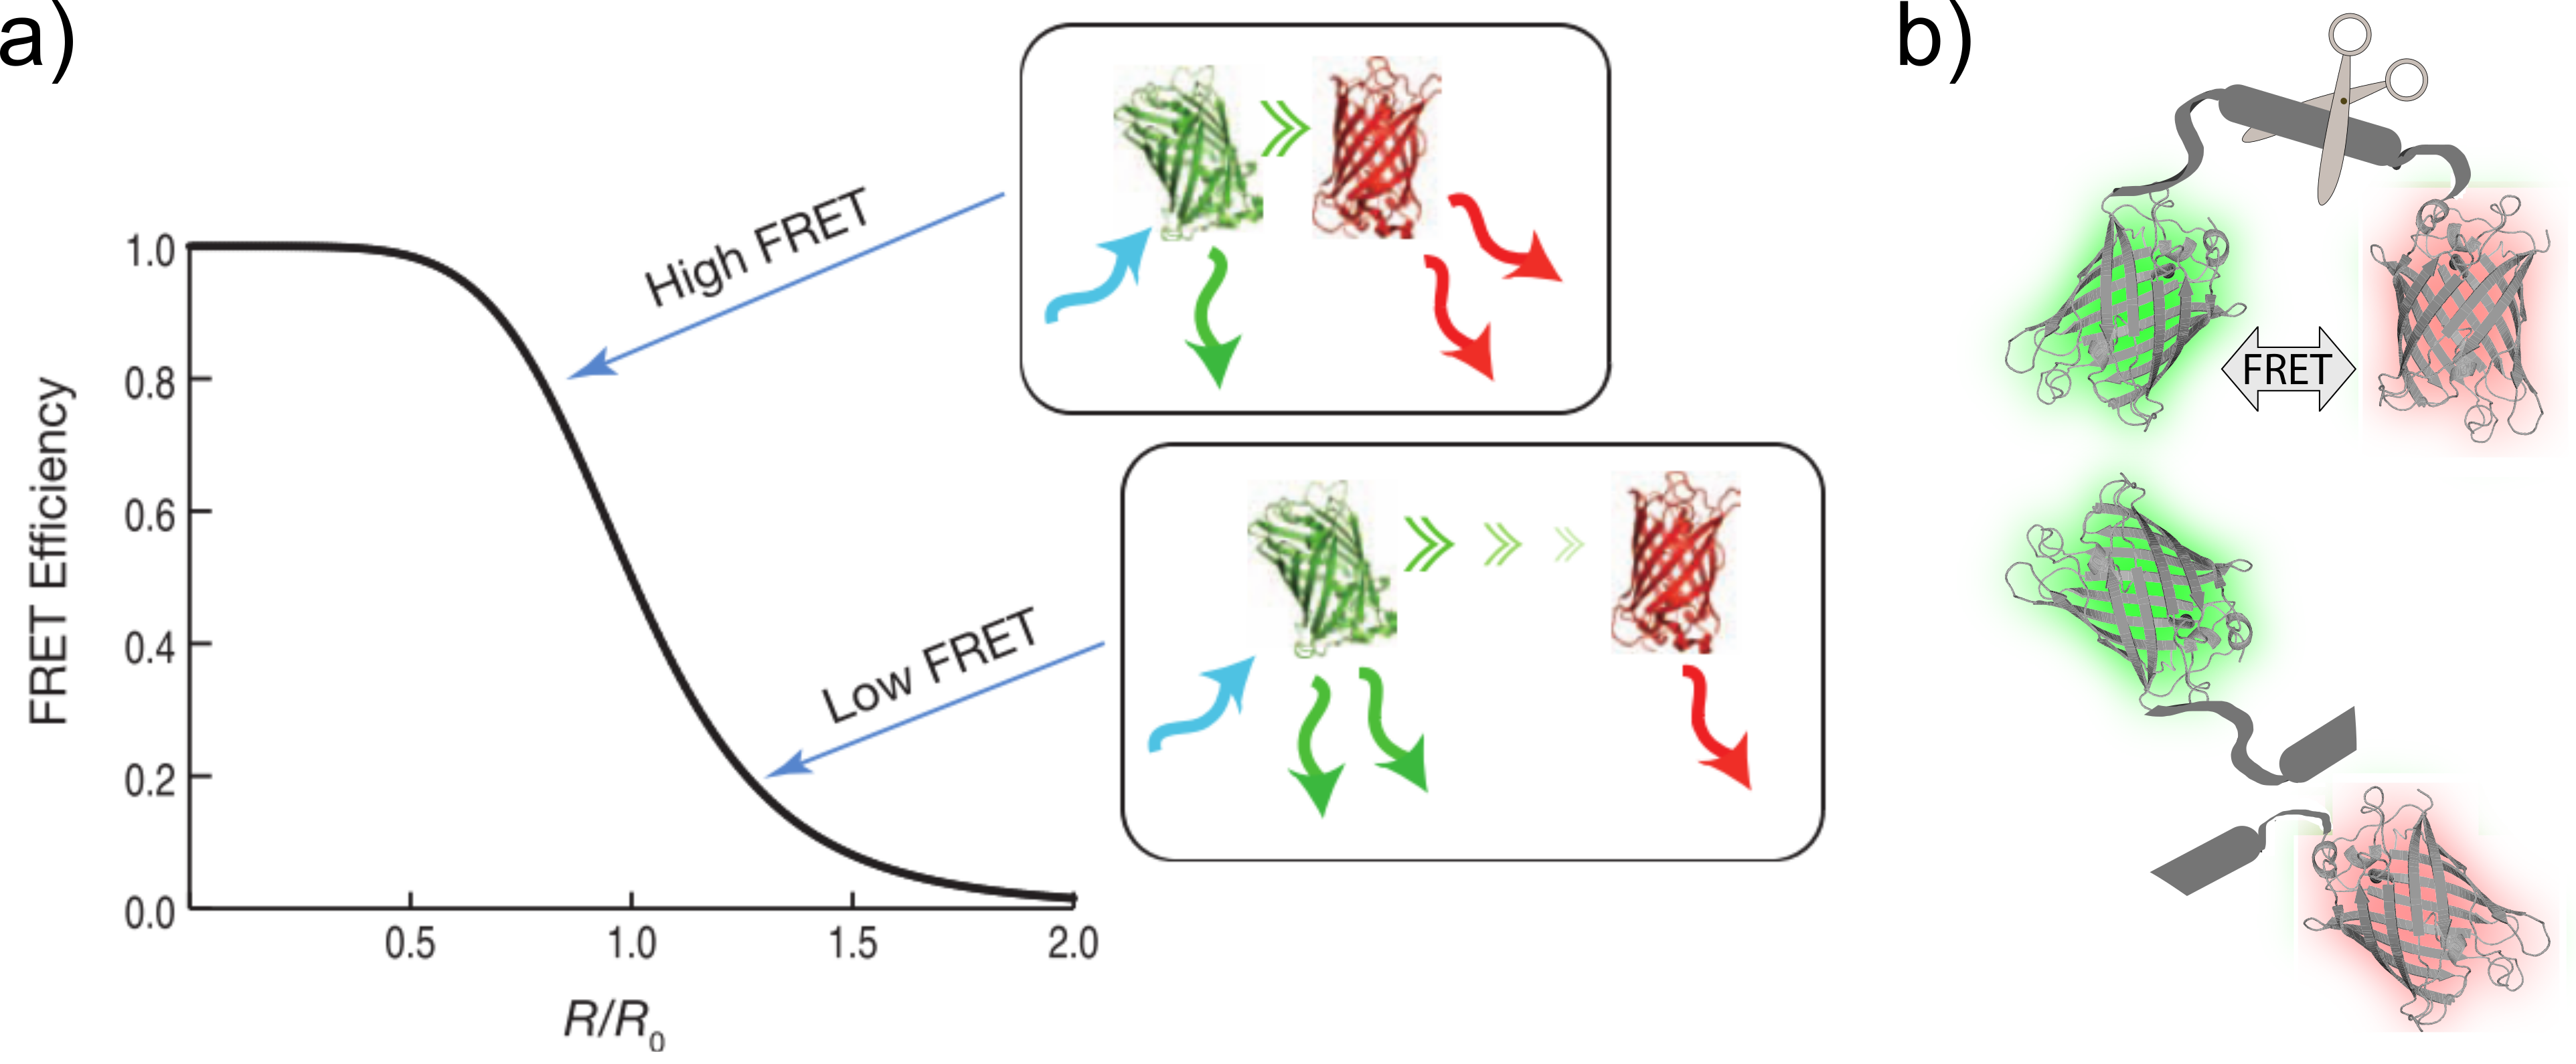
\includegraphics[width=0.9\textwidth]{./img/FRETClivaje.png}
    \caption{\textbf{a)} Curva que muestra la eficiencia de la transferencia de energía de resonancia de Förster según la separación entre los fluoróforos. $R_0$ es la separación en la que la eficiencia es de un $50\%$\cite{GreccoBastiaens2009}. \textbf{b)} Esquema de la interrupción de energía producida por el clivaje del sensor diseñado.}
    \label{fig:FRET}
\end{figure}

El tiempo de vida de fluorescencia provee información sobre el estado del fluoróforo y su ambiente molecular. Con FLIM pueden generarse mapas de tiempos de vida de fluorescencia que son sensibles a condiciones ambientales como pH y reacciones del estado de excitación como FRET\cite{Grecco2009}. Aprovechando el hecho de que la combinación de FRET y FLIM forman una técnica robusta para observar modificaciones postraduccionales en proteínas \textit{in situ}, \textit{Grecco et al.}\cite{Grecco2010} lo utilizan para identificar componentes de la red de señalización producida por el factor de crecimiento epidermal (\textit{EGF}).

FRAP fue desarrollada originalmente en la década de 1970 para medir motilidad de proteínas\cite{Ishikawa-Ankerhold2012}. Esta técnica toma ventaja del hecho de que fluoróforos dejan de emitir fluorescencia cuando son expuestos a ciclos sucesivos de excitación y emisión, fenómeno denominado fotoblanqueo. En los experimentos de FRAP, se fotoblanquea una región de interés para generar dos subpoblaciones de fluoróforos separados espacialmente. Midiendo la variación de la intensidad en el tiempo, se puede estimar la motilidad de proteínas fluorescentes\cite{Carrero2003}, además de las fracciones de proteínas móviles e inmóviles (ver figura \ref{fig:FRAP}). \textit{Carrero et al.}\cite{Carrero2003} explican claramente como obtener información acerca de las constantes de difusión de proteínas en estudio, además de constantes de asociación y disociación.

\begin{figure}
    \centering
    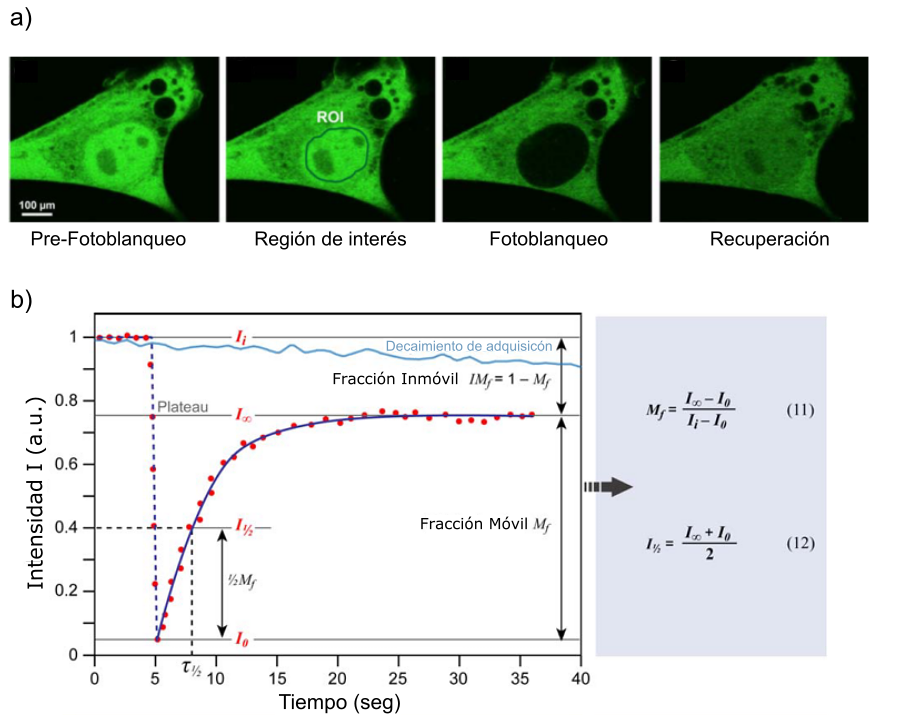
\includegraphics[width=0.80\textwidth]{./img/FRAP.png}
    \caption{Ejemplos de la técnica de recuperación de fluorescencia posterior a fotoblanqueo (FRAP)\cite{Ishikawa-Ankerhold2012}. \textbf{a)} Imágenes del procedimiento utilizado en FRAP. \textbf{b)} Curva típica obtenida en FRAP a partir de la cual puede estimarse las fracciones móvil e inmóvil de la proteína marcada.}
    \label{fig:FRAP}
\end{figure}

Una variación de FRAP, FLIP, consiste en fotoblanquear una región específica repetidas veces y observar la disminución en la intensidad de fluorescencia en otras regiones, permitiendo estudiar conectividad entre compartimentos. Esta técnica fue utilizada por \textit{Cole et al.}\cite{Cole1996} para estudiar el transporte entre los sacos del aparato de Golgi. Para ello fotoblanqueaban proteína verde fluorescente (GFP) unida a $\beta$-1,4-galactosyltransferasa y estudiaban la disminución de intensidad de fluorescencia en el mismo saco, así como también en los contiguos, en distintas condiciones celulares\cite{Cole1996}.

La técnica de FLAP es una extensión de FLIP donde se utilizan dos fluoróforos distintos unidos. Uno de los fluoróforos es fotoblanqueado mientras que el otro se utiliza como reportero. Estudiar la diferencia entre las señales de ambos fluoróforos permitió a \textit{Dunn et al.}\cite{Dunn2002} deducir de oligomerización de $\beta$-actina (proteína constitucional de los filamentos de actina del citoesqueleto celular)\cite{Dunn2002}. Resultados análogos pueden obtenerse al utilizar fluoróforos fotoactivables. Estos son fotoactivados en cierta región y se observa la variación en intensidad de fluorescencia en la región fotoactivada y otra de interés\cite{Ishikawa-Ankerhold2012}.

\begin{figure}
    \centering
    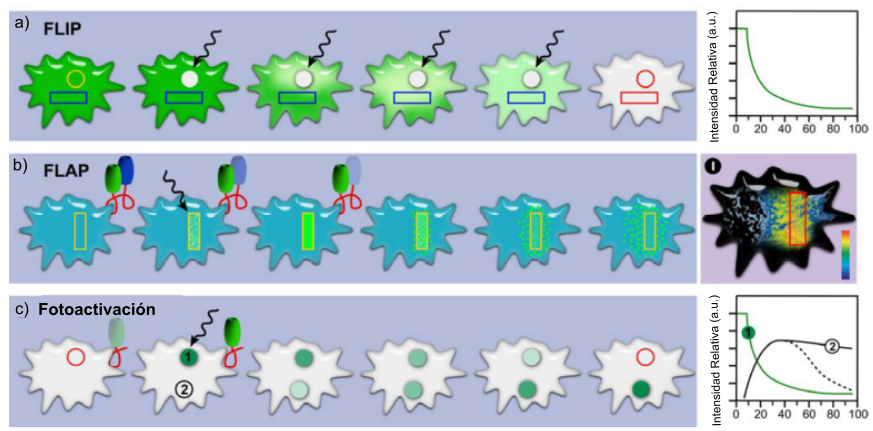
\includegraphics[width=0.90\textwidth]{./img/FLIPetc.png}
    \caption{Ejemplos de técnicas de microscopía de fluorescencia(FRAP)\cite{Ishikawa-Ankerhold2012}. \textbf{a)} FLIP consiste en fotoblanquear sucesivas veces una región y estudiar como decae la fluorescencia en el resto de la célula o compartimentos. \textbf{b)} FLAP es una técnica análoga a FRAP donde se usan dos fluoróforos. La señal a analizar es la diferencia entre el fluoróforo fotoblanqueado y el reportero unido que no es fotoblanqueado. \textbf{c)} Los fluoróforos fotoactivables pueden ser encendidos en una región para luego estudiar su migración hacía otra.}
    \label{fig:FLIP}
\end{figure}

Los métodos de fluorescencia disponibles actualmente facilitan los análisis en biología de sistemas ya que permiten observar las propiedades espaciales y dinámicas de sistemas vivos con mínimas perturbaciones. De esta forma, la actividad enzimática puede ser visualizada cuantitativamente en células vivas para ser posteriormente combinada con modelado matemático y así revelar regulación espacial y comportamiento dinámico del sistema\cite{Verveer2008}. 


%%%%%%%%%%%%%%%%%%%%%%%%%%%%%%%%%%%%%%%%%%%%%%
\section{Sistema Biológico}

La apoptosis es un proceso de muerte celular programada ordenado por el que la célula muere ante estímulos extra o intracelulares. Este proceso es fundamental tanto para el desarrollo embriológico de órganos y sistemas, como para el mantenimiento de la homeostasis del número de células, entre otras cosas. Es un proceso finamente regulado que cuando se altera produce graves patologías como malformaciones o aparición de tumores, así como también enfermedades neurodegenerativas por citar algunos ejemplos\cite{Kominami2012}. Por otro lado, cuando la célula no puede responder adecuadamente al estímulo recibido, esta puede derivar en necrosis, un proceso de muerte desordenado que genera una serie de reacciones locales, conduciendo a respuestas de tipo inflamatorio que son probablemente la manifestación más importante de este proceso. Entender el mecanismo de inducción de apoptosis, sin generar elevados niveles de necrosis, es importante en la generación de tratamientos para enfermedades como el cáncer.

Los engranajes principales de la maquinaria apoptótica son las caspasas. Estas pertenecen a una familia de proteínas denominado cisteín-proteasas y se encargan de seccionar proteínas reconociendo una secuencia específica de aminoácidos. Para gatillar la cascada de caspasas que desencadena la apoptosis se pueden estimular dos vías diferentes, intrínseca y extrínseca, que producen dinámicas distintas en el sistema. La vía intrínseca surge de señales provenientes de adentro de la célula, como estrés celular o daño al ADN, mientras que, la vía extrínseca es desencadenada por estimulación de receptores de membrana celular llamados receptores de la muerte\cite{Sakamaki2012}.

En circunstancias normales, las caspasas se hallan expresadas constitutivamente en su forma inactiva como zymógenos o procaspasas. Su activación se encuentra regulada en numerosos puntos, siendo necesario por lo tanto una cascada de eventos para que la célula se vea irreversiblemente determinada a la apoptosis. En respuesta a las señales proapoptóticas, una primer familia de caspasas, denominadas iniciadoras (caspasa-8, -9, entre otras), son activadas. Estas a su vez activan un segundo grupo de caspasas, llamadas efectoras (caspasa-3, -6 ó -7), encargadas de desmantelar la célula\cite{Varner2000}.

\begin{figure}
    \centering
    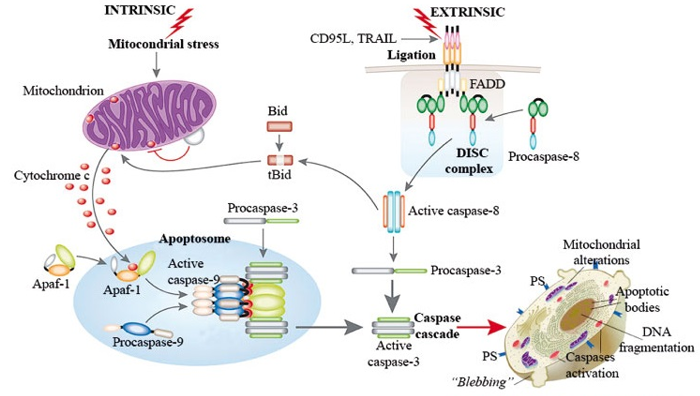
\includegraphics[width=0.90\textwidth]{./img/caspasa0.png}
    \caption{Esquema de las vías de iniciación de la apoptosis. Puede apreciarse que tanto la vía extrínseca como la intrínseca culminan en la activación de la caspasa-3, y subsecuentemente en la degradación del proteoma y el material genético, produciéndose la muerte celular. Se debe destacar también el acoplamiento entre ambas vías generado por la caspasa-8\cite{FotoVias}.}
    \label{fig:Vias}
\end{figure}

En el caso de la vía extrínseca, la cascada de eventos comienza a nivel de la membrana celular cuando se forman los complejos de señalización de la inducción de muerte (\textit{DISC}) en respuesta a la activación de los receptores de muerte. A continuación, las caspasas iniciadoras (-8 y -10) son activadas por dimerización forzada por DISC, para que estas a su vez cliven la procaspasa efectora (-3), activándola\cite{Albeck2008}. Simultáneamente, la caspasa-8 acopla las vías extrínseca e intrínseca\cite{Harrington2008}. Análogamente, la vía intrínseca es iniciada posterior a injuria celular con la diferencia que la caspasa iniciadora en este caso es la caspasa-9. Una vez inicializada esta vía, se permeabiliza la membrana celular mitocondrial para luego formarse el apoptosoma, encargado de reclutar y activar la procaspasa-9\cite{Harrington2008}.

Ambas vías convergen finalmente en la activación de las caspasas efectoras (-3, -6 o -7). Estas últimas se encargan de degradar directamente el proteoma, y activar ADNasas para luego desmantelar los cromosomas de células determinadas a morir. Dado que la activación de caspasas constituye un cambio irreversible en el destino de la célula, este se halla regulado en varios niveles, desde la formación de complejos entre los receptores celulares, unión de miembros de la familia de Bcl-2 pro- y anti-apoptóticos tanto en la mitocondria como en el citosol, la traslocación de Smac y citocromo c de la mitocondria al citosol hasta la represión directa de caspasas por parte de proteínas inhibidoras de la apoptosis (\textit{IAP})\cite{Albeck2008}.

%Published models of cell death control usually focus on one death pathway only, such as the apoptotic extrinsic or intrinsic pathways [2],[3],[4]. A few studies integrate both pathways [5], some show that the concentration of specific components contribute to the decision between death and survival [6],[7] while other studies investigate the balance between proliferation, survival or apoptosis in specific cell types along with the role of key components in these pathways [8], but no mathematical models including necrosis are available yet. Moreover, we still lack models properly demonstrating how cellular conditions determine the choice between necrosis, apoptosis and survival, and how and to what extent conversions are allowed between these fates.


%%%%%%%%%%%%%%%%%%%%%%%%%%%%%%%%%%%%%%%%%%%%%%
\section{Esquema de la Tesis}

En este trabajo se propone adaptar un modelo basado en ecuaciones diferenciales ordinarias acopladas que permita interpretar las señales fotofísicas observables experimentalmente durante la apoptosis. El modelo adapatado debe describir adecuadamente el comportamiento de los biosensores basados en FRET que se utilizaron. A partir de este modelo será posible, no solo comprender datos experimentales obtenidos de series temporales de imágenes de células apoptóticas, sino también realizar predicciones que sirvan para planear nuevos experimentos.
%integrar un modelo describa la dinámica de las caspasas durante la apoptosis

En el capítulo \ref{cap:microscopia} se presentan métodos de análisis que permiten evaluar el estado del ensamble de fluoróforos a partir de los observables fotofísicos experimentales. Primero se presenta una explicación teórica sobre el origen de la señal de anisotropía en polarización para luego poder comprender los métodos de análisis que se presentarán.

A continuación, el capítulo \ref{cap:modelo} muestra como se diseña el modelo matemático que describe el sistema biológico en estudio y de donde surgen los parámetros utilizados. Luego, se explican las adaptaciones realizadas para incluir en el modelo el comportamiento de los biosensores utilizados. Se concluye el capítulo con el desarrollo de un método que permite obtener información valiosa sobre el estado del sistema a partir del conocimiento del estado de los sensores.

Por último, en el capítulo \ref{cap:informacion} se introducen los datos experimentales explicando su procedencia. Este conjunto de datos es analizado mediante los métodos presentados previamente y se sugieren algunas correcciones al protocolo experimental para facilitar análisis futuros. Finalmente, se confecciona un estudio estadístico con el objetivo de contrastar los datos experimentales analizados con las predicciones del modelo teórico confeccionado.


%%%%%%%%%  Microscopia
\chapter{Microscopía de Anisotropía en la Fluorescencia}
\label{cap:microscopia}

%Los fluoróforos suelen clasificarse según sean intrínsecos o extrínsecos. Los intrínsecos ocurren naturalmente dentro de los organismos como NADH, flavinoides, o clorofila. Frecuentemente, las moléculas de interés no son fluorescentes y es necesario marcarlas con reporteros extrínsecos, como fluoresceína, rodamina u otras. 

La fluorescencia es ideal para observar la ubicación de moléculas en células ya que es no poco invasiva y puede ser detectada con una elevada sensibilidad y especificidad. Lo que es más importante, las propiedades espectroscópicas pueden ser explotadas para obtener información, no solo de la ubicación del fluoróforo, sino también de su nanoambiente\cite{Bastiaens1999}. Los fluoróforos en general poseen en su estructura momentos de transición de absorción y emisión que se hallan subtendidos en direcciones específicas. Esto se aprecia fenomenológicamente como una emisión polarizada al excitar con luz linealmente polarizada. Por otro lado, la probabilidad de excitar un fluoróforo depende del ángulo entre el eje de polarización de la excitación y el momento de transición de excitación. Este fenómeno puede explicarse fácilmente si se representa al fluoróforo como una antena dipolar eléctrica.

Existen varios fenómenos que pueden tener un efecto depolarizante sobre la emisión del fluoróforo una vez excitado. En primer lugar, los momentos de transición de excitación y emisión no siempre son colineales, resultando en una depolarización de la emisión respecto a la excitación. Por otro lado, durante el tiempo de vida del estado excitado, éste puede rotar libremente contribuyendo así al efecto depolarizante. La polarización de la muestra se mide en términos de anisotropía. Como el tiempo de vida en el estado excitado es mayor o comparable a la escala temporal de la difusión rotacional de biomoléculas, estos suelen ser utilizados en biofísica. Es así que en la anisotropía de la muestra se ve reflejado el efecto del nanoambiente sobre estos fluoróforos, como por ejemplo la viscosidad del medio\cite{Lakowicz2006}.

%Al excitar una muestra de fluoróforos con luz polarizada, la emisión también resulta polarizada. Este fenómeno surge de la existencia de momentos de transición de absorción y emisión que se hallan subtendidos en direcciones específicas de las estructuras del fluoróforo. La polarización de la muestra se mide en términos de anisotropía.

%Debido a que la probabilidad de excitar un fluoróforo depende del ángulo entre el eje de polarización de la excitación y el momento transitorio de excitación, es de esperar que aquellas moléculas que se encuentran orientadas en el mismo sentido que la excitación sean excitadas preferentemente. Simultáneamente, la difusión rotacional de estos fluoróforos excitados producirán un efecto de depolarización que puede apreciarse como un aumento de anisotropía.

%%%%%%%%%%%%%%%%%
\section{Definición de Anisotropía}

Consideremos que se excita una muestra de fluoróforos con luz linealmente polarizada. Con fines introductorios y sin pérdida de generalidad podemos asumir que el eje de polarización para el haz incidente es paralelo al eje z. La anisotropía de la muestra se define como la razón entre las componentes polarizadas de emisión y su intensidad total, es decir,

\begin{equation}
    r = \frac{I_{z} - I_{y}}{I_{x} + I_{y} + I_{z}} = \frac{I_{z} - I_{y}}{I_{T}}.
    \label{eq:anisotropia_ejes}
\end{equation}

\noindent Si además tenemos en consideración el carácter simétrico\cite{Weber1965}, podemos apreciar que $I_x = I_y$. Experimentalmente, se utilizan analizadores para estudiar la intensidad de fluorescencia emitida por la muestra en el eje paralelo al de incidencia (I$_{\parallel}$), así como también en el eje perpendicular (I$_{\perp}$). Cabe destacar entonces que $I_x = I_y = I_{\perp}$ y $I_z = I_{\parallel}$, quedando la ecuación \ref{eq:anisotropia_ejes} expresada de la siguiente manera

\begin{equation}
    r = \frac{I_{\parallel} - I_{\perp}}{I_{\parallel} + 2 I_{\perp}}.
    \label{eq:anisotropia}
\end{equation}

\noindent Dado que esta magnitud adimensional es normalizada por la intensidad total de fluorescencia, es independiente de la concentración de fluoróforo utilizado.

\begin{figure}
    \centering
    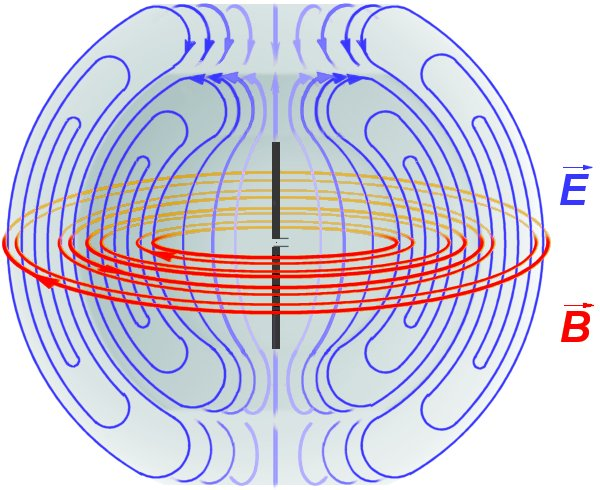
\includegraphics[width=0.33\textwidth]{./img/AntenaDipolar.jpg}
    \caption{Emisión radiativa de una antena dipolar. En azul ($\vec{E}$) se encuentra representado el campo eléctrico emitido, mientras que en rojo ($\vec{B}$) se muestra el campo magnético.}
    \label{fig:AntenaDipolar}
\end{figure}

\section{Teoría de Anisotropía}

La teoría de anisotropía puede explicarse fácilmente al considerar un único fluróforo. Por simplicidad consideremos que sus momentos de transición de excitación y emisión son colineales. La radiación de campo lejano emitida por el fluoróforo puede estudiarse mediante electrodinámica clásica y es análoga a un dipolo eléctrico (ver figura \ref{fig:AntenaDipolar}).

El campo eléctrico generado por un fluoróforo es

\begin{equation}
    E(\theta, \phi) = k \frac{\sin{ \theta}}{r} \hat{\theta},
\end{equation}

\noindent donde $k$ es la constante que determina la intensidad del dipolo eléctrico, $r$ la distancia al fluoróforo y se utilizó un sistema de coordenadas centrado en el fluoróforo cuyo eje z es compartido con la orientación del dipolo.

Por otro lado, si el dipolo no se encuentra alineado con el eje z, es fácil ver que la proyección del campo radiativo sobre el eje z será proporcional a $\cos{ \theta}$, mientras que sobre el eje x es proporcional a $\sin {\theta} \sin {\phi}$. Dichas proyecciones pueden apreciarse en la figura \ref{fig:RadiacionFluoroforo}.

\begin{figure}
    \centering
    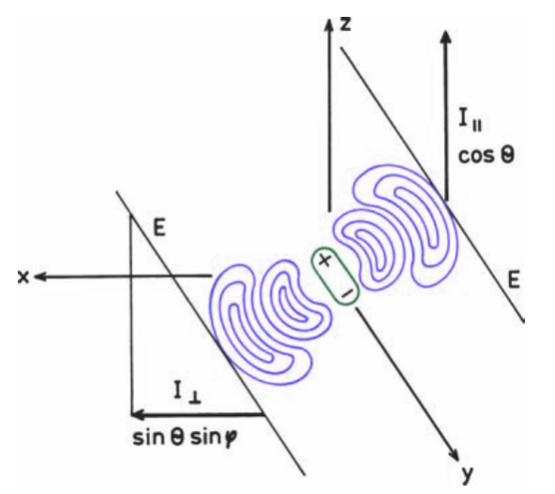
\includegraphics[width=0.4\textwidth]{./img/RadiacionFluoroforo.png}
    \caption{Emisión radiativa de un fluoróforo orientado al azar en un sistema de coordenadas esféricas. También se presentan las proyecciones en el eje z y eje x del campo irradiado\cite{Lakowicz2006}.}
    \label{fig:RadiacionFluoroforo}
\end{figure}

Una vez analizada la excitación y emisión de un único fluoróforo podemos comenzar a estudiar el comportamiento de un ensamble de estos ante la excitación con luz linealmente polarizada. Utilizando nuevamente argumentos de simetría, vemos que la probabilidad de excitar una molécula depende del ángulo $\theta$ que forma con el eje z, pero es independiente del ángulo $\phi$ que forma con el eje y. Luego, considerando que la intensidad de las proyecciones dependen

\begin{align}
    I_{\parallel} = & \cos^{2} \theta \label{eq:IntProyPar}\\
    I_{\perp}     = & \sin^{2} \phi \sin^{2} \theta, \label{eq:IntProyPerp}
\end{align}

\noindent y que podemos eliminar la dependencia con $\phi$ calculando el valor medio de $\sin^{2} \phi$ entre $0$ y $2\pi$, llegamos a

\begin{align}
    I_{\parallel} = & \cos^{2} \theta \label{eq:IntProyPar2}\\
    I_{\perp}     = & \frac{1}{2} \sin^{2} \theta. \label{eq:IntProyPerp2}
\end{align}

Analicemos ahora que sucede con la dependencia en $\theta$. Por generalidad, usaremos que $f(\theta) d\theta$ es la probabilidad de que una molécula se oriente entre $\theta$ y $\theta + d\theta$. Estimando las intensidades medidas a partir del promedio del ensamble apreciamos que

\begin{align}
    I_{\parallel} = & \int_0^{\pi/2} f(\theta) \cos^{2} \theta d\theta = k \langle \cos^{2} \theta \rangle \label{eq:IntProyPar3}\\
    I_{\perp}     = & \frac{1}{2} \int_0^{\pi/2} f(\theta) \sin^{2} \theta d\theta = \frac{k}{2} \langle \sin^{2} \theta \rangle. \label{eq:IntProyPerp3},
\end{align}

\noindent donde $k$ es una constante instrumental, que relaciona la intensidad del dipolo eléctrico con la ganancia de la cámara y otras características del sistema de detección. Reemplazando estas expresiones halladas en la ecuación \ref{eq:anisotropia} y utilizando identidades trigonométricas arribamos a

\begin{equation}
    r = \frac{3 \langle cos ^2 \theta \rangle - 1}{2}.
    \label{eq:anisotropiamedio}
\end{equation}

\noindent Cabe destacar que esta expresión es válida para ensambles con simetría alrededor del eje z. Además, entre las hipótesis utilizadas se planteó la colinealidad entre los momentos de transición de excitación y emisión, hecho que se cumple para muy pocas especies de fluoróforos pero que simplifica considerablemente los cálculos. Por último, se debe recalcar que $r$ se anula si el $\langle cos ^2 \theta \rangle = 1/3$, que, entre otros efectos, puede darse cuando el ángulo entre los momentos de excitación y emisión es de $54,7^{\circ}$. Este ángulo, llamado ángulo mágico también puede aprovecharse colocando el analizador horizontal $54,7^{\circ}$ respecto del vertical, y de esta forma se observa que $I_{\parallel} = 2 I_{\perp}$, ya que $\cos^{2} 54,7^{\circ} = 1/3$ y $\sin^{2} 54,7^{\circ} = 2/3$, resultando en que su suma sea proporcional a $I_{\parallel} + 2 I_{\perp}$. Esta disposición se utiliza para estudiar el decaimiento de intensidad de la muestra.

%En algunos casos, el objetivo es medir la intensidad total de fluorescencia y no la anisotropía de la muestra. Cuando este es el caso, los analizadores pueden colocarse de forma tal de obtener un valor proporcional a la intensidad total de fluorescencia independientemente de la anisotropía de la muestra. Si el analizador horizontal se ubica $54,7^{\circ}$ respecto del vertical, apreciamos que $I_{\parallel} = 2 I_{\perp}$, ya que $\cos^{2} 54,7^{\circ} = 1/3$ y $\sin^{2} 54,7^{\circ} = 2/3$, resultando en que su suma sea proporcional a $I_{\parallel} + 2 I_{\perp}$. Esta disposición se utiliza para estudiar el decaimiento de intensidad de la muestra.

A continuación, profundicemos sobre la dependencia de la distribución de probabilidad de los fluoróforos en $\theta$. Como se mencionó previamente, la probabilidad de excitar a un fluróforo es proporcional a $\cos^{2} \theta$, donde $\theta$ es el ángulo que el dipolo de excitación forma con el eje z (ver figura \ref{fig:FluoroforoExcitacion}). Además, el número de moléculas que forman un ángulo entre $\theta$ y $\theta + d\theta$ con el eje z es proporcional a $\sin{\theta} d\theta$, ya que se encuentran distribuidas completamente al azar. Combinando ambas estimaciones apreciamos que

\begin{equation}
    f(\theta) d\theta = \cos^{2} \theta \sin{ \theta} d\theta,
\end{equation}

\noindent resultando entonces en

\begin{equation}
    \langle \cos^{2} \theta \rangle = \frac{ \int_0^{\pi/2} f(\theta) \cos^{2} \theta d\theta} {\int_0^{\pi/2} f(\theta) d\theta} = \frac{3}{5}.
\end{equation}

\noindent Este último resultado aplicado a la ecuación \ref{eq:anisotropiamedio} implica una anisotropía máxima de $0,4$. Para llegar a este resultado se consideraron los dipolos de excitación y emisión como colineales, y no se tuvieron en cuenta efectos depolarizantes. Bajo estas condiciones se obtuvo $I_{\parallel} = 3 I_{\perp}$. Dado que esta es la anisotropía máxima que puede obtenerse de una muestra orientada al azar, cualquier valor medido superior es indicativo de artefactos en la observación\cite{Tramier2008}.

\begin{figure}
    \centering
    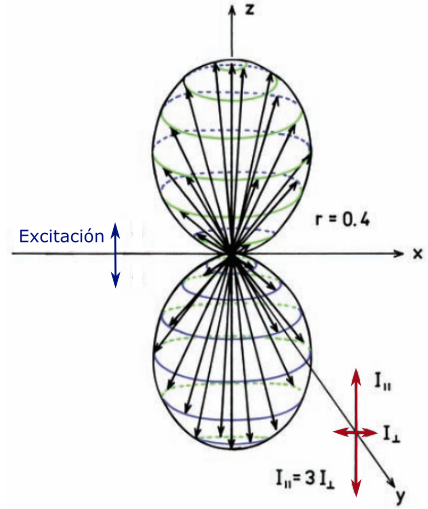
\includegraphics[width=0.4\textwidth]{./img/FluoroforoExcitacion.png}
    \caption{Distribución de fluoróforos excitados al utilizar luz linealmente polarizada en el eje z. Puede apreciarse la simetría del sistema alrededor de este eje\cite{Lakowicz2006}.}
    \label{fig:FluoroforoExcitacion}
\end{figure}

%\begin{figure}
%    \centering
%    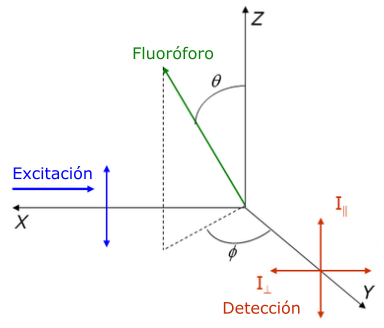
\includegraphics[width=0.4\textwidth]{./img/FluoroforoOrientado.png}
%    \caption{Proyecciones de un fluoróforo orientado al azar en el espacio\cite{Lakowicz2006}.}
%    \label{fig:FluoroforoOrientado}
%\end{figure}

Por último, es necesario recalcar que si en la muestra se encuentran más de una especie de fluoróforos, la anisotropía observada será

\begin{equation}
    r = \sum_i f_i r_i,
    \label{eq:anisotropiamezcla}
\end{equation}

\noindent donde $f_i$ es la fracción de intensidad de una especie, y $r_i$ su anisotropía\cite{Jablonski1960}. Esto resulta de considerar el carácter lineal de las intensidades emitidas por los fluoróforos, es decir,

\begin{equation}
    r = \frac{\sum_i I_i r_i}{\sum_i I_i}.
    \label{eq:anisotropiaInt}
\end{equation}


%%%%%%%%%%%%%%%%%%%%%%%%%%%%%%%%%%%%
\section{Métodos de Medición}

Los métodos de adquisición de datos para realizar análisis de anisotropía en polarización de fluorescencia se clasifican en formato de L ó T, según se utilicen uno o dos canales de emisión respectivamente. Estos métodos se aplican tanto a fluorímetros como a microscopios ópticos.


\begin{figure}
%    \begin{subfigure}{0.43\textwidth}
%            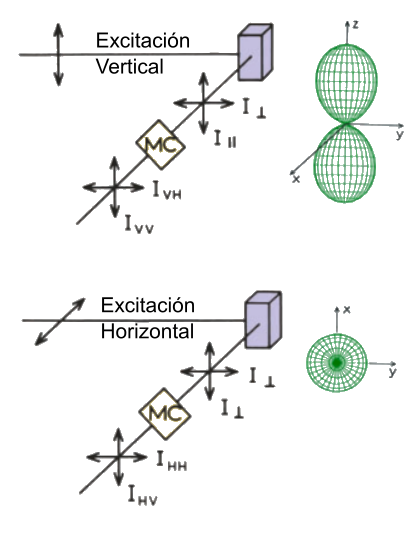
\includegraphics[width=0.99\textwidth]{./img/LFormat.png}
%            \caption{Esquema de la disposición en formato de L del sistema de adquisición. En esta disposición se adquieren los datos de ambas intensidades de manera secuencial.}
%            \label{fig:LFormat}
%    \end{subfigure}
%    ~
%    \begin{subfigure}{0.43\textwidth}
%        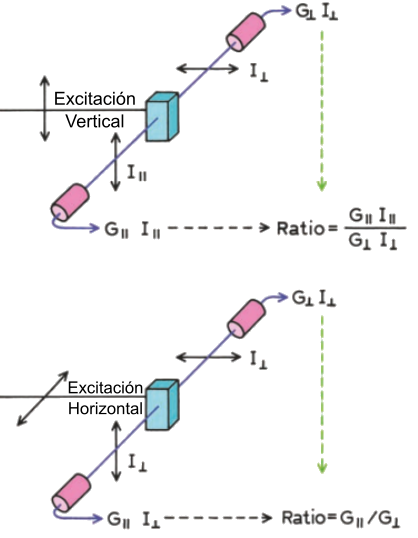
\includegraphics[width=0.99\textwidth]{./img/TFormat.png}
%        \caption{Esquema de la disposición en formato de T del sistema de adquisición. En esta disposición se adquieren datos de ambas intensidades simultáneamente.}
%        \label{fig:TFormat}
%    \end{subfigure}
    \centering
    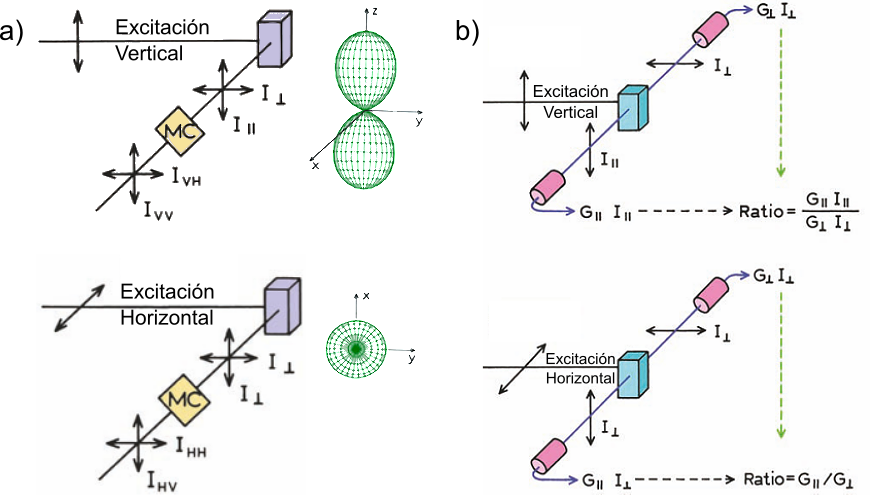
\includegraphics[width=0.9\textwidth]{./img/Formats.png}
    \caption{Disposiciones experimentales utilizadas para adquisición de datos en anisotropía de fluorescencia\cite{Lakowicz2006}. \textbf{a)}: Esquema de la disposición en formato de L del sistema de adquisición. En esta disposición se adquieren los datos de ambas intensidades de manera secuencial. \textbf{b)}: Esquema de la disposición en formato de T del sistema de adquisición. En esta disposición se adquieren datos de ambas intensidades simultáneamente.}
    \label{fig:Formats}
\end{figure}

\subsection{Formato de L o de Canal Único}

La disposición en forma de L es la más utilizada comúnmente ya que se necesita un único canal de emisión. Consiste en incidir sobre la muestra con luz linealmente polarizada y observar su emisión por medio de un monocromador y un analizador, como se muestra en la figura \ref{fig:Formats}a.

Desde el punto de vista experimental, la sensibilidad del sistema para observar intensidad de fluorescencia en ambos ejes puede ser distinta. Dado que el objetivo es obtener mediciones de $I_{\parallel}$ e $I_{\perp}$, procedemos a calcularlos a partir de las observaciones realizadas. En primer lugar, tenemos acceso a las intensidades cruzadas que son proporcionales a las intensidades buscadas de la forma

\begin{align}
    I_{VV} =& k S_V I_{\parallel} \\
    I_{VH} =& k S_H I_{\perp},
\end{align}

\noindent donde $k$ es una constante instrumental y $S_V$ y $S_H$ las sensibilidades de ambas disposiciones del analizador. El subíndice de las intensidades observadas corresponden: el primero a la orientación del eje de polarización del haz de excitación y el segundo al de emisión observado, siendo $V$ vertical, y $H$ horizontal.

Puede apreciarse rápidamente que la relación entre ambas intensidades nos devuelve

\begin{equation}
    \frac{I_{VV}}{I_{VH}} = \frac{S_V}{S_H} \frac{I_{\parallel}}{I_{\perp}} = G \frac{I_{\parallel}}{I_{\perp}},
\end{equation}

\noindent donde $G$ corresponde a cuanto más sensible es un canal respecto del otro, es decir, da cuenta de las depolarizaciones introducidas por el sistema óptico en cuestión y no por la muestra. Se debe notar que es necesario conocer el valor de $G$ para obtener las intensidades buscadas. Con este objetivo en mente, es fácil mostrar que utilizando una haz de excitación polarizado horizontalmente hallamos

\begin{equation}
    \frac{I_{HV}}{I_{HH}} = \frac{S_V}{S_H} \frac{I_{\perp}}{I_{\perp}} = G,
\end{equation}

\noindent ya que al rotar el eje de polarización de la excitación, se rota también el la distribución de los estados excitados de forma tal que en la observación solo se observan las $I_{\perp}$, como se muestra en la figura \ref{fig:Formats}a.

La anisotropía de la muestra se puede calcular a partir de las observaciones realizadas utilizando

\begin{equation}
    \frac{I_{VV}}{I_{VH} G} = \frac{I_{VV}}{I_{VH}} \frac{I_{HV}}{I_{HH}} = \frac{I_{\parallel}}{I_{\perp}},
\end{equation}

\noindent y, por lo tanto,

\begin{equation}
    r = \frac{I_{\parallel}/I_{\perp} - 1}{I_{\parallel}/I_{\perp} +2},
    \label{eq:r1}
\end{equation}

\noindent que es análogo a

\begin{equation}
    r = \frac{I_{VV}-GI_{VH}}{I_{VV}+2GI_{VH}}.
    \label{eq:r2}
\end{equation}

\subsection{Formato de T o de Dos Canales}

En la disposición en forma de T se utilizan dos canales de emisión para adquirir los valores de intensidad de fluorescencia simultáneamente. En esta disposición, los polarizadores de emisión no se rotan durante la medición y, por lo tanto, no cambia su sensibilidad. Además, la velocidad de adquisición de datos es mayor ya que se observan ambos canales al mismo tiempo.

De manera análoga a la disposición en forma de L, se obtienen los relaciones entre las intensidades medidas, $R_V$ y $R_H$

\begin{align}
    R_V =& \frac{G_{\parallel} I_{\parallel}}{G_{\perp} I_{\perp}} \\
    R_H =& \frac{G_{\parallel}}{G_{\perp}},
\end{align}

\noindent donde $G_{\parallel}$ and $G_{\perp}$ son las sensibilidades correspondientes a cada canal. Por último, calculando la relación entre ambas llegamos a

\begin{equation}
    \frac{R_V}{R_H} = \frac{I_{\parallel}}{I_{\perp}},
\end{equation}

\noindent expresión que podemos combinar con las ecuaciones \ref{eq:r1} y \ref{eq:r2} para calcular la anisotropía buscada. Se debe recalcar que esta metodología tiene dificultades cuando alguna de las intensidades de fluorescencia es muy baja.

\subsection{Implementación en Microscopía}

Es posible implementar en un microscopio óptico común un arreglo de polarizadores que permita obtener información sobre la anisotropía en la polarización de fluorescencia. Estos sistemas, denominados microscopios de imágenes de anisotropía de fluorescencia, permiten obtener mapas de anisotropía de diversas muestras.

\begin{figure}
    \centering
    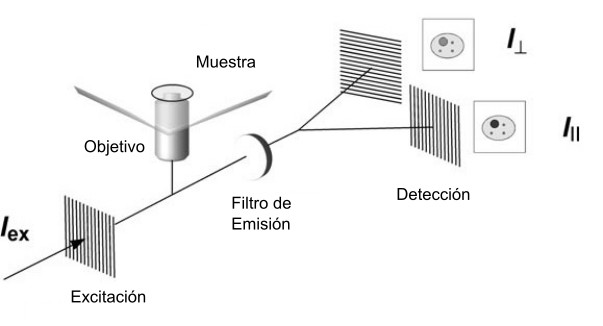
\includegraphics[width=0.6\textwidth]{./img/EsquemaAnisotropia.png}
    \caption{Esquema del armado experimental utilizado para observar anisotropía en microscopía óptica. Se aprecia que el canal de excitación y emisión es el mismo y se utiliza un espejo dicroico para separar ambas señales\cite{Chan2011}.}
    \label{fig:EsquemaMicro}
\end{figure}

La implementación de anisotropía de fluorescencia en microscopía puede clasificarse también según se utilicen uno o dos canales de emisión. Las adaptaciones incluyen un polarizador entre la fuente y la muestra, y otro entre la muestra y la cámara de adquisición, como se muestra en la figura \ref{fig:EsquemaMicro}. En algunos casos, se utilizan cristales birefringentes (por ejemplo: calcita) para separar las componentes paralela y perpendicular de la emisión, y visualizarlas al mismo tiempo mediante la cámara\cite{Yao2010}.

La cuantificación de anisotropía de fluorescencia en microscopía presenta varios desafíos. Muchos de los componentes presentes en un microscopio inducen depolarización de la luz que si no es corregida adecuadamente conlleva a errores sistemáticos\cite{Chan2011}. En primer lugar, las lentes objetivo utilizadas comúnmente tienen amplitud numérica elevada. Esto último genera una mezcla de distintas polarizaciones ya que los conos de luz de excitación y emisión son subtendidos en un amplio ángulo sólido en el punto de muestreo (ver figura \ref{fig:NA})\cite{Andreev1993}.

\begin{figure}
    \centering
    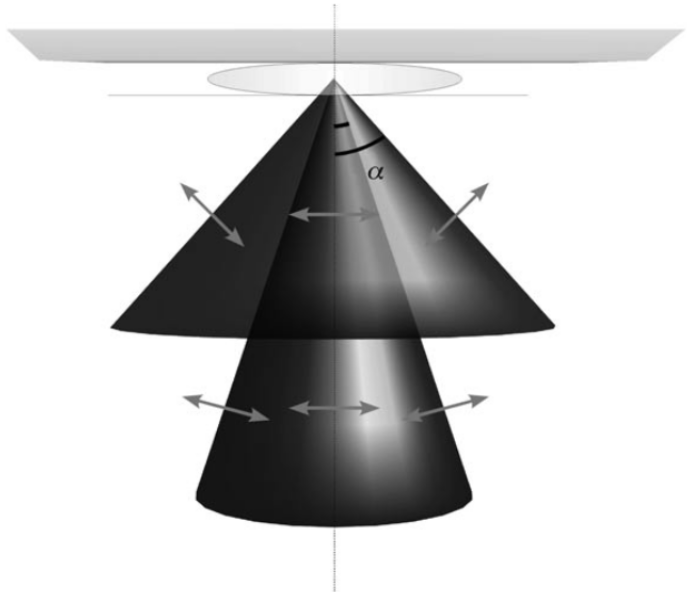
\includegraphics[width=0.4\textwidth]{./img/NA.png}
    \caption{Depolarización producida por lentes objetivo con amplitud numérica alta. El cono de luz en el punte de observación tiene un ángulo sólido mayor para lentes con apertura numérica más grande, mezclando las polarizaciones verticales con las horizontales\cite{Chan2011}.}
    \label{fig:NA}
\end{figure}

Por otro lado, se debe destacar que la disposición de los haces de luz de excitación y emisión no permiten clasificar al sistema en las disposiciones descriptas previamente. En este caso, el camino óptico del haz de excitación es el mismo que el de emisión. Esto último vuelve inviable la posibilidad de medir $I_{\perp}$ en ambos ejes de polarización, obligando a utilizar un valor de anisotropía de referencia para calibrar el sistema.

Con el objetivo de corregir las posibles depolarizaciones generadas por el sistema óptico del microscopio, se pueden comparar las anisotropias observadas mediante microscopía con las obtenidas por medio de un fluorímetro comercial. Simultáneamente, se requiere la calibración del factor G que tiene en cuenta las diferencias en sensibilidad del sistema para polarizaciones cruzadas. El factor G puede hallarse a partir de un valor de referencia de anisotropía de un fluoróforo utilizando la ecuación

\begin{equation}
    G = \frac{I_{\parallel} (1 - r_{ref})}{I_{\perp} (1 + 2r_{ref})},
\end{equation}

\noindent donde $r_{ref}$ es el valor de anisotropía conocido de la muestra. Dado que el factor G es dependiente de la longitud de onda utilizada, se debe calibrar para el rango utilizado en el experimento.



%%%%%%%%%%%%%%%%%%%%%%%%%%%%%%%%%%%%
\section{Factores Depolarizantes}

Con el objetivo de aprovechar al máximo las ventajas que proveen las técnicas de anisotropía de fluorescencia, debemos conocer primero las fuentes de depolarización. Estas pueden provenir de características intrínsecas al fluoróforo, como es el desplazamiento angular que existe entre el dipolo de excitación y el de emisión, así como también por causas extrínsecas, como son la difusión rotacional y la transferencia de energía de resonancia\cite{Lakowicz2006}.

El carácter dipolar del fluoróforo nos permite estudiar la orientación de estructuras subcelulares. El desplazamiento angular entre el dipolo de excitación y el de emisión nos introduce una depolarización que debe ser tenida en cuenta a la hora de estudiar dichas orientaciones. En la figura \ref{fig:GFPDipole} se presentan imágenes de cristales de proteína verde fluorescente donde se aprecian las distintas intensidades de fluorescencia en las distintas polarizaciones. Estudiar las intensidades emitidas mientras se rotan los polarizadores de excitación y emisión permiten detectar los ejes de ambos dipolos\cite{Inoue2002}.

\begin{figure}
    \centering
    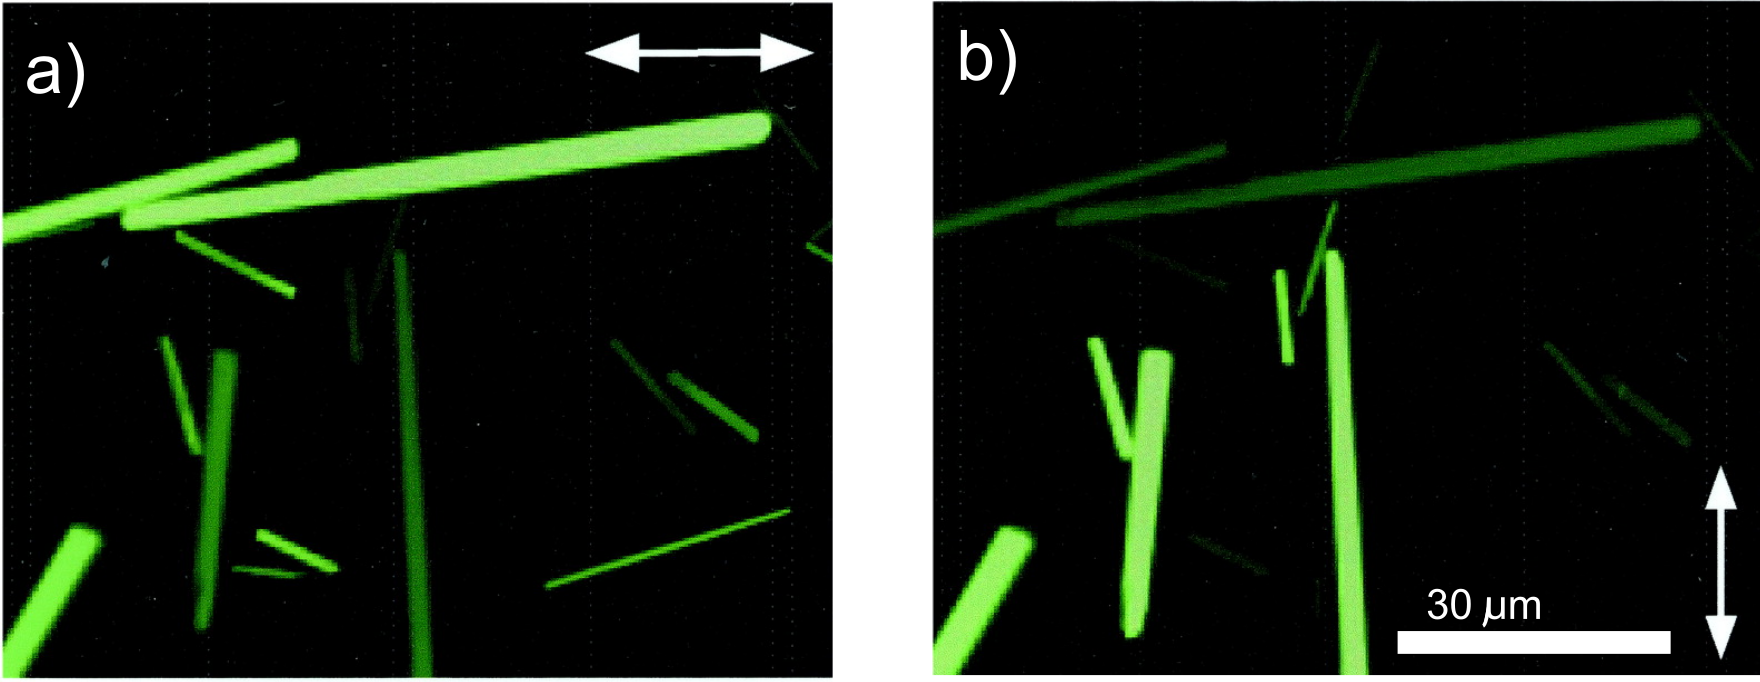
\includegraphics[width=0.8\textwidth]{./img/GFPDipole.png}
    \caption{Cristales de proteínas verde fluorescente\cite{Inoue2002}. Se excitaron las muestras con luz linealmente polarizada en ambos casos (orientada según las flechas) y no se utilizó analizador en ningún caso.}
    \label{fig:GFPDipole}
\end{figure}

Estudiar la orientación del fluoróforo unido a la cabeza de myosina (S$_1$) permitió identificar su disposición y orientación al unirse a F-actina. En el trabajo de \textit{Borejdo et al.}\cite{Andreev1993}, se concluyó que S$_1$ podía unirse de dos formas distintas según se halle en exceso o déficit en relación a la cantidad de F-actina.

La difusión rotacional es producto de las rotaciones del fluoróforo mientras este se encuentra en el estado excitado. Su efecto sobre la anisotropía surge a partir del juego entre el tiempo de vida de fluorescencia y el tiempo de correlación de rotación. Entre los factores que afectan el tiempo de correlación de rotación se encuentran la viscosidad del medio en que se halla disuelto el fluoróforo, el tamaño de este, y si se encuentra unido a otras moléculas (ver figura \ref{fig:DifusionRotacional}). 

\begin{figure}
    \centering
    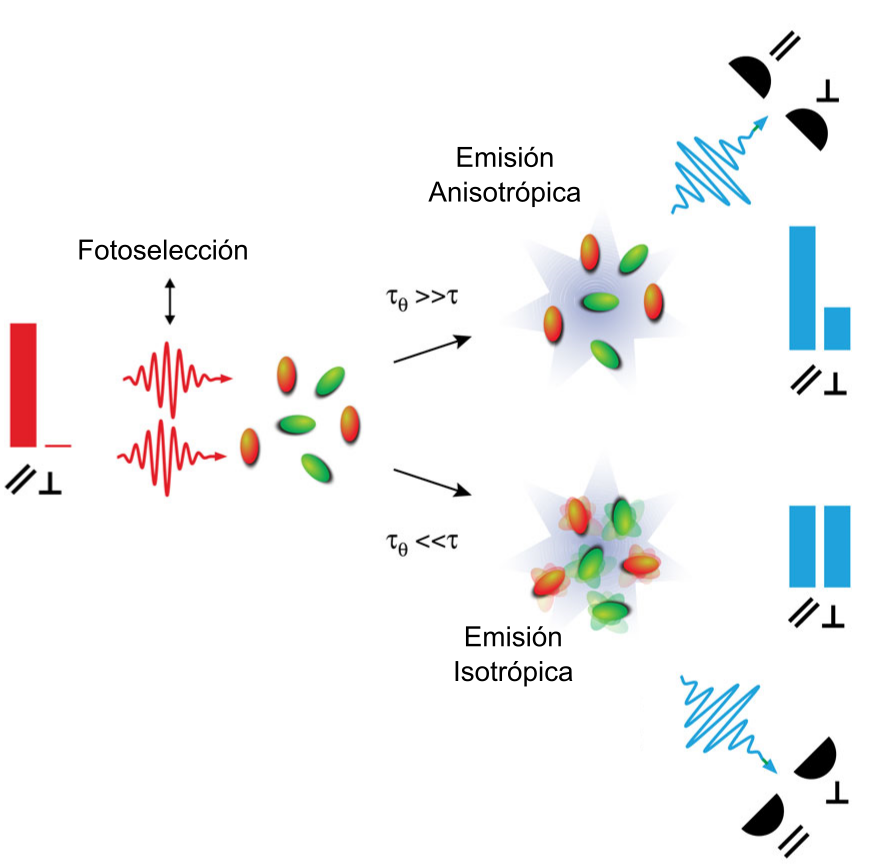
\includegraphics[width=0.6\textwidth]{./img/DifusionRotacional.png}
    \caption{Esquema del efecto que tiene la difusión rotacional sobre la anisotropía de fluorescencia. Se realiza una fotoselección incidiendo con luz linealmente polarizada y se observa una emisión anisotrópica cuando el tiempo de correlación de rotación es considerablemente mayor al de vida media de la fluorescencia, o emisión isotrópica si la situación es la inversa\cite{Dubach2014}}
    \label{fig:DifusionRotacional}
\end{figure}

Conociendo el efecto que tiene la viscosidad del medio sobre el tiempo de correlación de rotación del fluoróforo, la anisotropía de fluorescencia puede ser utilizada para obtener información sobre parámetros reológicos del citosol, como se muestra en el trabajo de \textit{Verkman et al.}\cite{Swaminathan1997}. Por otro lado, dado que la unión del fluoróforo a otra molécula produce un cambio en la anisotropía, se la puede utilizar para reportar la proporción de fluoróforos ligados entre el total de fluoróforos. La ecuación \ref{eq:anisotropiamezcla} y conocer los valores específicos de anisotropía de cada estado permiten hallar esta proporción. \textit{Weissleder et al.}\cite{Dubach2014} utilizan esta técnica \textit{in vivo} para observar la dinámica de interacción entre la droga y su blanco (Olaparib) en tiempo real, mostrando su utilidad para descifrar la dinámica intracelular.

%Por último, otros factores que producen depolarización son la transferencia de energía de resonancia y la dispersión. La transferencia de energía de resonancia se produce en soluciones muy concentradas, en estas la distancia entre fluoróforos es comparable a la distancia característica $R_0$. Estas concentraciones generalmente son considerablemente mayores a las utilizadas normalmente, del orden miliMolar. Por otro lado, algunas muestras biológicas pueden ser turbias produciendo dispersión de fotones que afectan de forma distinta la anisotropía según se produzca antes o después de excitar al fluoróforo.

%%%%%%%%%%%%%%%%%%%%%%%%%%%%%%%%%
\section{Transferencia de Energía de Resonancia de Förster}

Cuando dos fluoróforos se encuentran próximos entre si, la energía de radiación puede ser transferida de forma no radiativa de uno a otro como resultado de acoplamiento dipolo-dipolo\cite{GreccoBastiaens2009}. Este fenómeno, denominado transferencia de energía de resonancia de Förster (FRET), puede ser explicado mediante electrodinámica clásica. La utilización generalizada de FRET se debe a que la distancia característica de esta transferencia es típicamente del orden del tamaño de una proteína o grosor de la membrana plasmática, hecho que lo vuelve valioso para estudiar colocalización e interacción molecular en escalas inferiores a la resolución del microscopio, así como también actividad enzimática\cite{Lakowicz2006}.

La transferencia de energía ocurre entre una molécula donante en el estado excitado y una aceptora en el estado fundamental. Las moléculas donante tienen menor longitud de onda de emisión y en general se solapa con la de excitación de la aceptora, como se muestra en la figura \ref{fig:EspectroFRET}\cite{Lakowicz2006}. La eficiencia del flujo de energía se define como

\begin{equation}
    E = \frac{1}{1+ \left( r/R_0 \right)^6},
\end{equation}

\noindent donde $r$ es la separación entre fluoróforos y $R_0$ es la distancia a la cual la mitad de la energía de excitación es transferida. Notar que si la concentración de fluoróforos es del orden miliMolar, la separación entre estos es del orden de $R_0$.

La separación $R_0$ puede ser calculada teóricamente a partir de la tasa de transferencia de energía de resonancia. Realizando los cálculos correspondientes se llega a que $R_0$ medido en \AA es

\begin{equation}
    R_0=(\kappa^2 \times J(\lambda) \times n^{-4} \times Q_D)^{1/6}\times 9.78 \times 10^3,
\end{equation}

\noindent donde $\kappa$ es la orientación relativa de los dipolos de ambos fluoróforos, $J(\lambda)$ es el solapamiento en los espectros de emisión y excitación del donante y aceptor (ver figura \ref{fig:EspectroFRET}), $n$ es el índice de refracción del medio y $Q_D$ es el rendimiento cuántico del dador\cite{Lakowicz2006}.

Hasta ahora hemos considerado la transferencia de energía entre dos fluoróforos distintos, denominado heteroFRET, pero esta puede ocurrir entre fluoróforos del mismo tipo si los espectros de emisión y excitación se superponen. Este caso, denominado homoFRET, se caracteriza por tener corrimiento en longitud de onda de Stokes suficientemente pequeños y elevados coeficientes de extinción (ver figura \ref{fig:EspectroFRET}b, propiedades que culminan en separaciones $R_0$ de alrededor de 57\AA\cite{Lakowicz2006}. En este caso, se analizan los cambios en la anisotropía de la muestra en lugar de la transferencia de energía entre distintos canales espectrales. En el trabajo de \textit{Stegemann et al.} se utiliza un sensor basado en homoFRET que es clivado por la caspasa-3 activa. Este se utiliza para estudiar la inicialización de apoptosis en respuesta a especies reactivas del oxígeno generadas mediante superficies fotofuncionales\cite{Grecco2015}.

\begin{figure}
\centering
    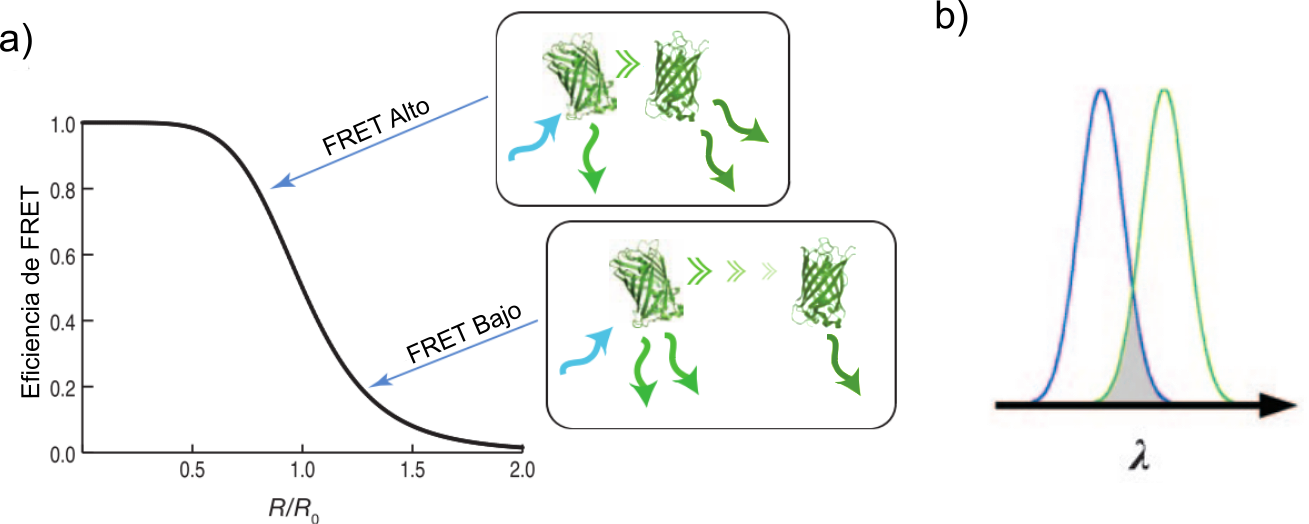
\includegraphics[width=0.8\textwidth]{./img/FRETAnisotropia.png}
    \caption{La Eficiencia de FRET depende de varios factores. \textbf{a)} Se muestra la eficiencia de FRET en función de la separación de fluoróforos. $R_0$ es la separación a la cual la eficiencia se reduce a la mitad. \textbf{b)} La superposición entre los espectros de emisión y el de excitación permiten que haya FRET entre ambos fluoróforos idénticos.}
    \label{fig:EspectroFRET}
\end{figure}

Entre las ventajas que presenta homoFRET respecto de heteroFRET se encuentra que la utilización de un único tipo de fluoróforo por sensor permite reducir el ancho espectral ocupado por cada sensor y así colocar más tipos de reporteros en cada célula. Análogamente, es posible utilizar fluoróforos distintos cuyo espectro sea suficientemente similar como para que ocurre homoFRET entre ambos, o mejor dicho seudo-homoFRET. Seleccionar cuidadosamente la pareja de fluoróforos es crucial para que el sensor confeccionado sea óptimo.

%En particular, se utilizaron biosensores que consistían en dos fluoróforos unidos por secuencias específicas de aminoácidos que son seccionadas por las caspasas, cuya actividad enzimática se desea estudiar. Con el objetivo de reportar la actividad de ambas vías iniciadoras, intrínseca y extrínseca, así como también la actividad de la caspasa efectora se utilizaron tres biosensores distintos de homoFRET. La ventaja que presenta este método respecto de heteroFRET es que la utilización de un único tipo de fluoróforo por sensor permite reducir el ancho espectral ocupado por cada sensor y así colocar más tipos de reporteros en cada célula.

%Los pares de fluoróforos utilizados fueron mCitrine-mCitrine, mCerulean-tagBFP y mKate2-mCherry. Es importante recalcar que los últimos dos pares, aunque están conformados por fluoróforos distintos, sus espectros son tan similares que no pueden ser diferenciados fácilmente y por esa razón se estudian mediante homoFRET.


%%%%%%%%%%%%%%%%%%%%%%%%%%%%%%%%%%%
\section{Análisis de Anisotropía en la Polarización}

Habiendo visto los conceptos teóricos, podemos estudiar como obtener información del estado del ensamble de fluoróforos a partir de la anisotropía observada. Comencemos por analizar un único par de fluoróforos distintos optimizados para homoFRET. La anisotropía observada puede hallarse mediante la ecuación \ref{eq:anisotropiaInt}

\begin{equation}
r = \frac{\sum_i I_i r_i}{\sum_i I_i}, \tag{\ref{eq:anisotropiaInt}}
\end{equation}

\noindent donde esta es el promedio pesado por las intensidades correspondientes al sensor en estado dimérico y monomérico de las anisotropías respectivas. 

Por otro lado, es importante notar que la intensidad observada de un fluoróforo en estado monomérico no será la misma que cuando este en estado dimérico. Dado que los distintos fluoróforos poseen propiedades fotofísicas diferentes, como sus espectros de absorción y emisión, su rendimiento cuántico, entre otras, sus brillos por molécula detectados serán diferentes. Luego, cuando estas se hallan en forma dimérica y ocurre FRET entre ellas, las intensidades observadas son distintas a cuando se hayan por separado ya que al trasmitirse energía entre ellas, los canales de detección detectarán intensidades distintas. Por otro lado, aunque se trate la misma especie de fluoróforo, la maduración de este puede no ser igual para ambos monómeros constituyentes, presentando el mismo fenómeno. De esta forma, las intensidades del sensor en cada estado pueden expresarse como


\begin{align}
    I_M &= b_M M\\
    I_D &= b_D 2D,
\end{align}

\noindent siendo $b_D$ y $b_M$ los brillos de un monómero de fluoróforo unido a otro o separado, respectivamente. $M$ y $D$ son las concentraciones de monómeros y dímeros, mientras que $I_M$ e $I_D$ dan cuenta de su intensidad.

En una primera aproximación al problema, podemos hacer el experimento mental de considerar distintas cubetas con variadas concentraciones, relativas y totales, de un tipo de sensor en sus distintos estados. Por simplicidad, podemos darle un orden temporal a las cubetas, que posteriormente nos ayudará a comprender lo que sucede dentro del sistema biológico.

Luego, supongamos que se tiene una única cubeta con una cantidad fija de sensores. Dado que la cantidad de monómeros es constante, podemos afirmar

\begin{equation}
    C = M + 2D,
    \label{eq:C_cte}
\end{equation}

\noindent hecho que nos permitirá expresar todo en función de la proporción de fluoróforo en estado monomérico ($m=M/C$). Es así que la ecuación \ref{eq:anisotropiaInt} puede reescribirse como

\begin{equation}
    r = \frac{I_M r_M + I_D r_D}{I_M+I_D} = \frac{b_M M r_M + b_D 2D r_D}{b_M M+b_D 2D} = \frac{m r_M + b (1-m) r_D}{m+b (1-m)},
    \label{eq:AnisotropiaFromParams}
\end{equation}

\noindent donde se tomó factor común $b_M C$ en el numerador y denominador, y se uso que $2D = C - M$. Las anisotropías correspondientes a los estados monoméricos y diméricos se denominaron $r_M$ y $r_D$, respectivamente. Por otro lado, $b = b_D/b_M$ representa la relación entre el brillo del monómero en cada estado y $m$ es la proporción de fluoróforo en estado monomérico, por lo que se encuentra entre $0$ y $1$. La expresión hallada nos permite vincular la anisotropía medida con la proporción de fluoróforo en cada estado.

A continuación, supongamos que en algún momento se desencadena una reacción enzimática que comienza a clivar y separar los dímeros en sus monómeros constitutivos. De esta forma, la curva de proporción de monómero respecto a la cantidad total de fluoróforo tendrá una forma sigmoidea o boltzmanniana como se muestra en la figura \ref{fig:m_sim}. El momento en que comienza la reacción, así como su tasa, son parámetros que definen distintas curvas y serán elegidos arbitrariamente por ahora. Además, la proporción de fluoróforo inicial en estado dimérico, como la proporción de monómeros al final de la reacción también deben ser determinados arbitrariamente, en particular, asumamos que iniciamos el experimento con todo el fluoróforo disponible en estado dimérico, pero culminamos la reacción con solo el 80$\%$ del fluoróforo en estado monomérico.

\begin{figure}
\centering
    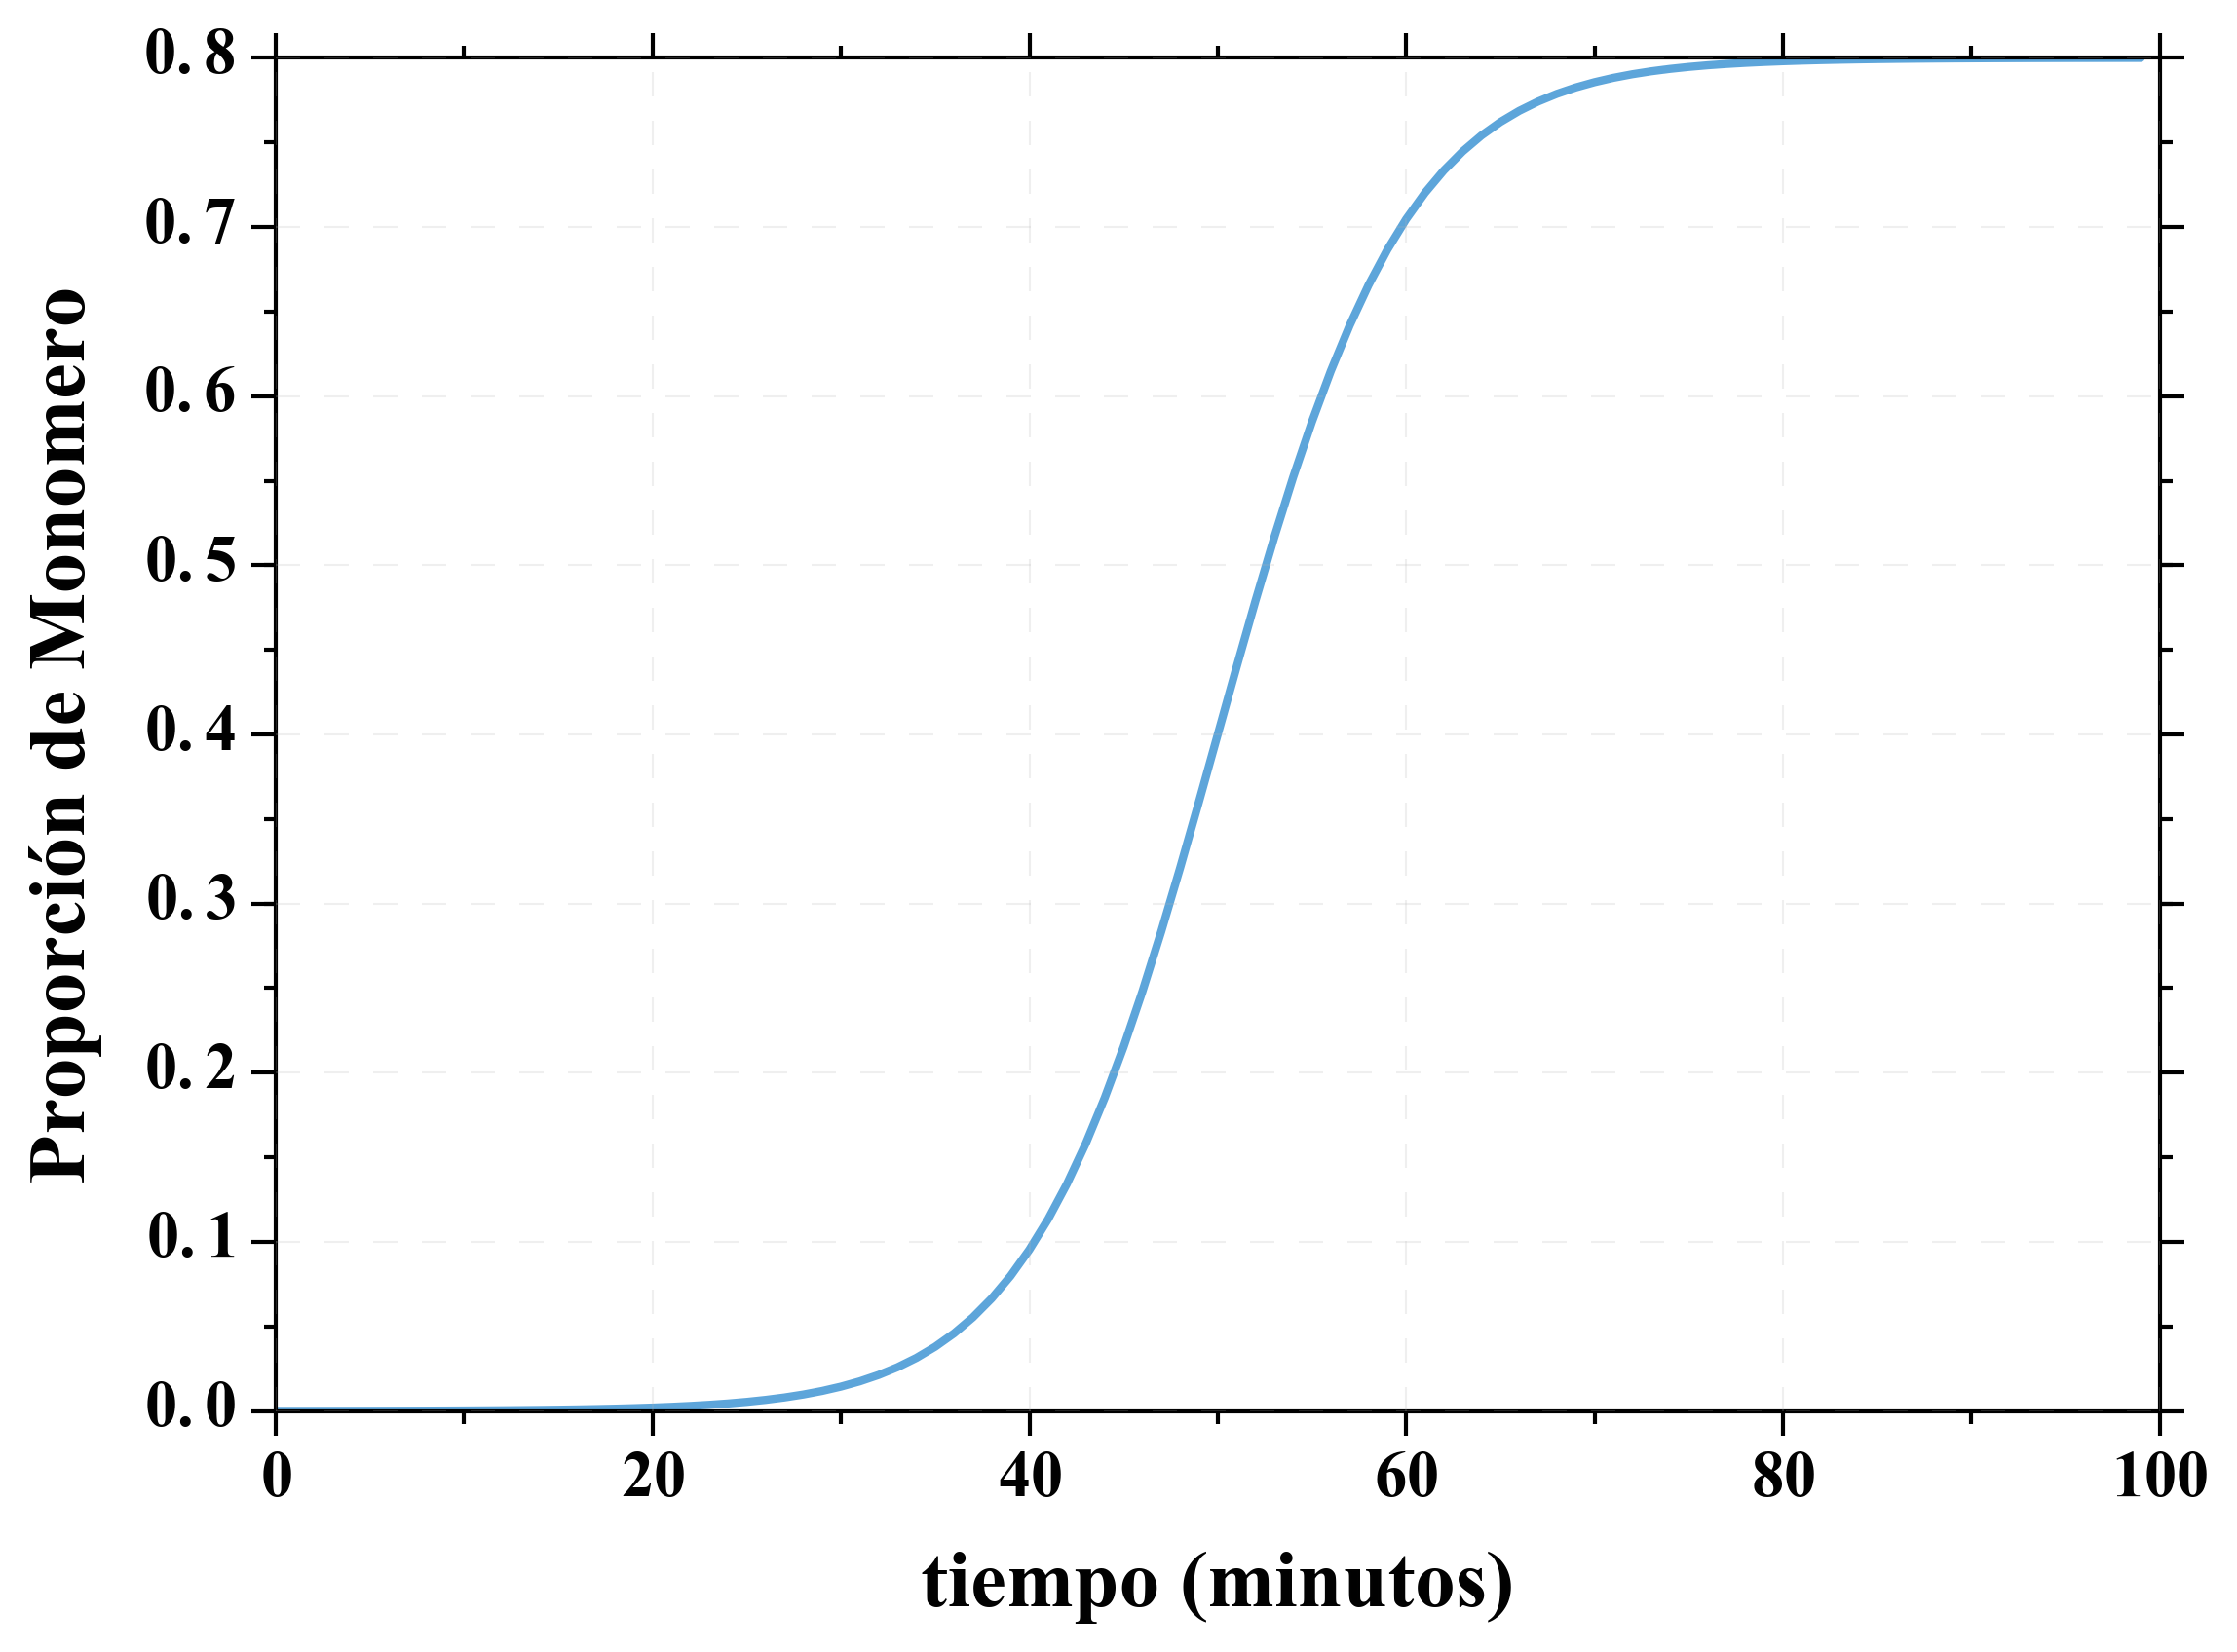
\includegraphics[width=0.6\textwidth]{./img/m_sim.png}
    \caption{Curva típica de variación de la proporción de sensores en estado monomérico simulada. Se determinó arbitrariamente que previo a la reacción todo el sensor se halle en estado monomérico, mientras que al final solo el $80\%$ se halla clivado.}
    \label{fig:m_sim}
\end{figure}

Si conocemos la proporción de fluoróforos en cada estado para cada cubeta, o mejor dicho, para cada tiempo, podemos calcular la anisotropía utilizando la ecuación \ref{eq:AnisotropiaFromParams}. Además de la proporción, es necesario conocer las anisotropías correspondientes a cada estado, así como también la relación entre brillos ($b$) para poder realizar el cálculo. Utilizando $m(t)$ simulado previamente y asumiendo que se trata del sensor de mCitrine-mCitrine, cuyas anisotropías teóricas son $r_D=0.221$ y $r_M=0.303$, se confeccionaron las distintas curvas de anisotropía. Por último, se realizó un barrido en el valor de $b$ desde $0.2$ a $0.8$ para confeccionar la figura \ref{fig:aniso_sim}. Se seleccionó este rango de valores de $b$ ya que se sabe experimentalmente que $b_M>b_D$, por lo que $0<b<1$. Se debe recalcar como el valor de $b$ cambia levemente la pendiente, así como el máximo valor de anisotropía alcanzado.

\begin{figure}
\centering
    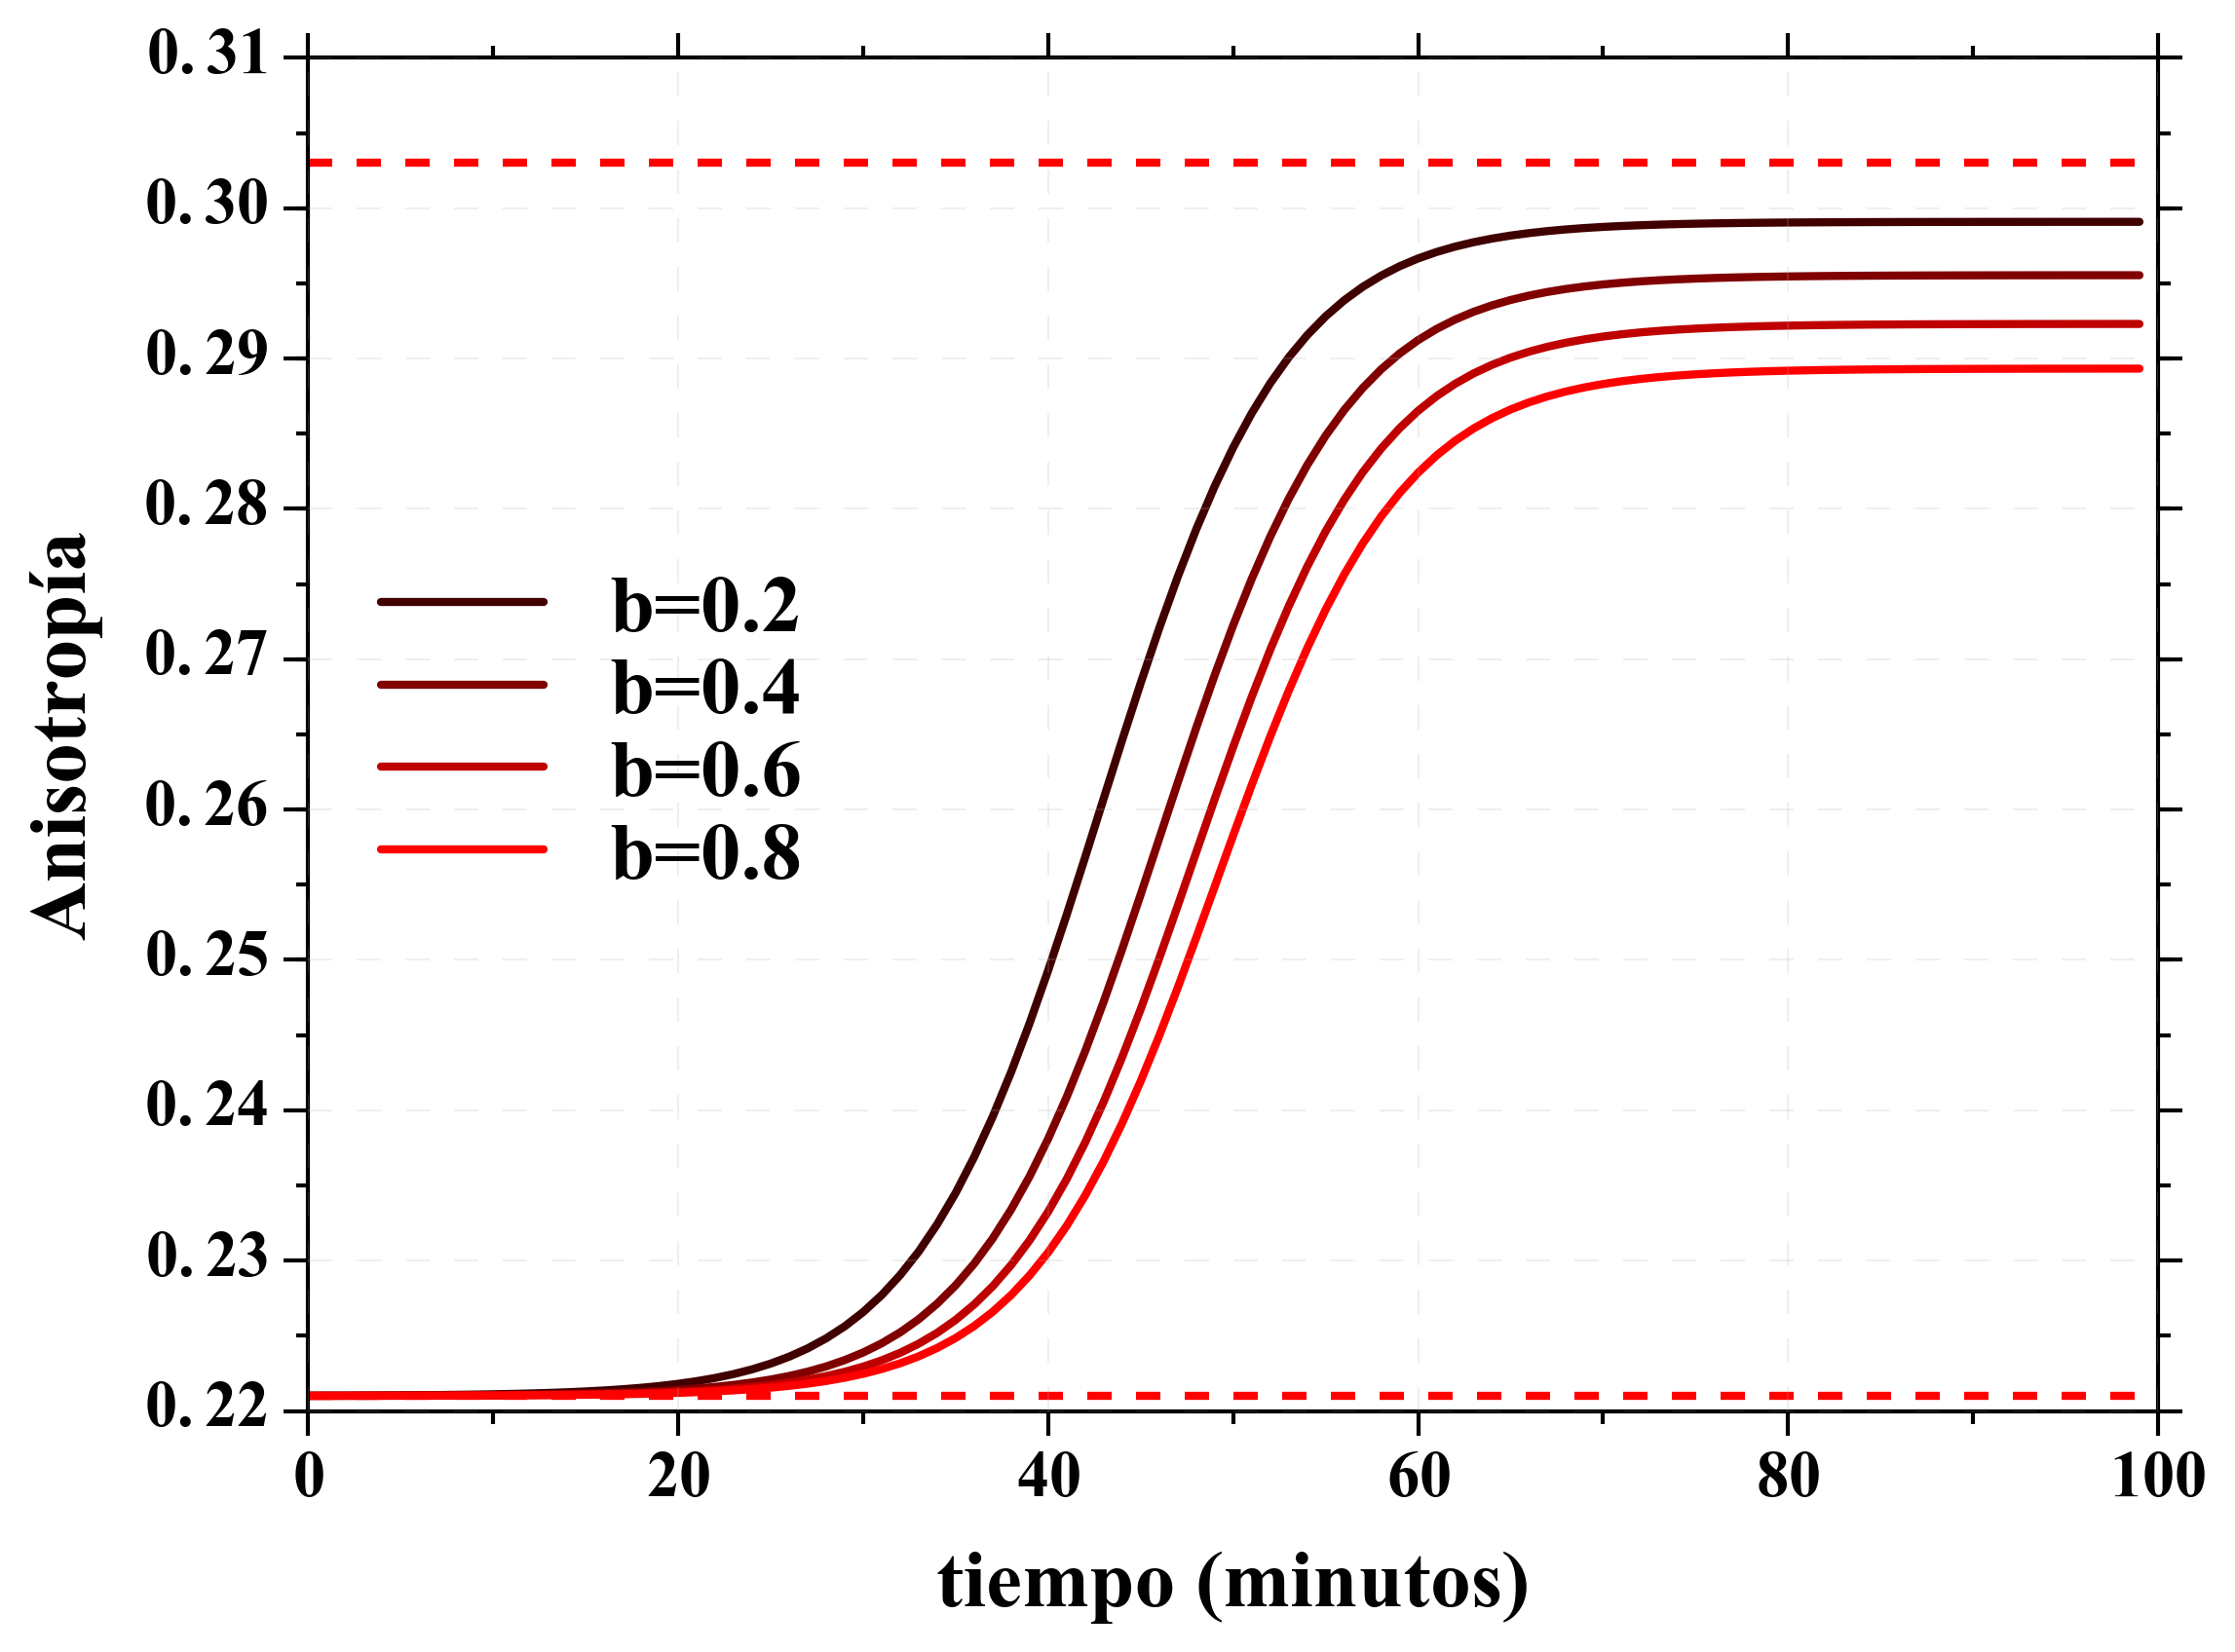
\includegraphics[width=0.6\textwidth]{./img/r_sim.png}
    \caption{Curva de anisotropía generada a partir de la curva simulada para $m$ considerando al fluróforo en cuestión como mCitrine. Se utilizaron $r_D=0.221$ y $r_M=0.303$, mientras que para el valor de $b$ se realizó un barrido entre $0.2$ y $0.8$. Las anisotropías del monómero y dímero se graficaron para remarcar los máximos y mínimos de anisotropía observabeles.}
    \label{fig:aniso_sim}
\end{figure}

Es interesante notar en la figura \ref{fig:aniso_sim} la relación entre los parámetros $b$ y $r_D$, ya que vemos que disminuir $b$ aumenta el máximo de anisotropía alcanzado cuando se cliva el $80\%$ del sensor. Esto quiere decir que podría disminuir $r_D$ o variar la proporción máxima clivada para obtener la misma curva. Esta relación entre parámetros complica el análisis a la hora de ajustar curvas ya que más de una combinación de parámetros devuelven curvas muy similares. Además, se aprecia que cuando no todo el fluoróforo es clivado, el hecho de utilizar fluoróforos distintos nos permite mejorar el rango dinámico del sensor.

Por otro lado, sabiendo que el brillo del fluoróforo es distinto en cada estado, podemos estudiar la fluorescencia total emitida para obtener información sobre el valor de $b$. Sin ir más lejos, el denominador en la ecuación \ref{eq:AnisotropiaFromParams} es igual a la intensidad total de fluorescencia emitida, es decir,

\begin{equation}
    I_T = I_M+I_D = b_M M+b_D 2D = b_M C (m+b (1-m)), \label{eq:Int_fromFit}
\end{equation}

\noindent donde $b_M C$ sirve de factor escala y representa la intensidad máxima de fluorescencia que puede alcanzarse si todo el sensor es clivado. Esto hecho puede verificarse viendo que si $m=1$, $I_T=b_M C$, sumado al hecho de que C representa la cantidad total de fluoróforo y $b_M$ es el brillo del fluoróforo en estado monomérico. Se grafican en la figura \ref{fig:f_sim} las curvas de fluorescencia total observada para el barrido en $b$ confeccionado previamente.

\begin{figure}
\centering
    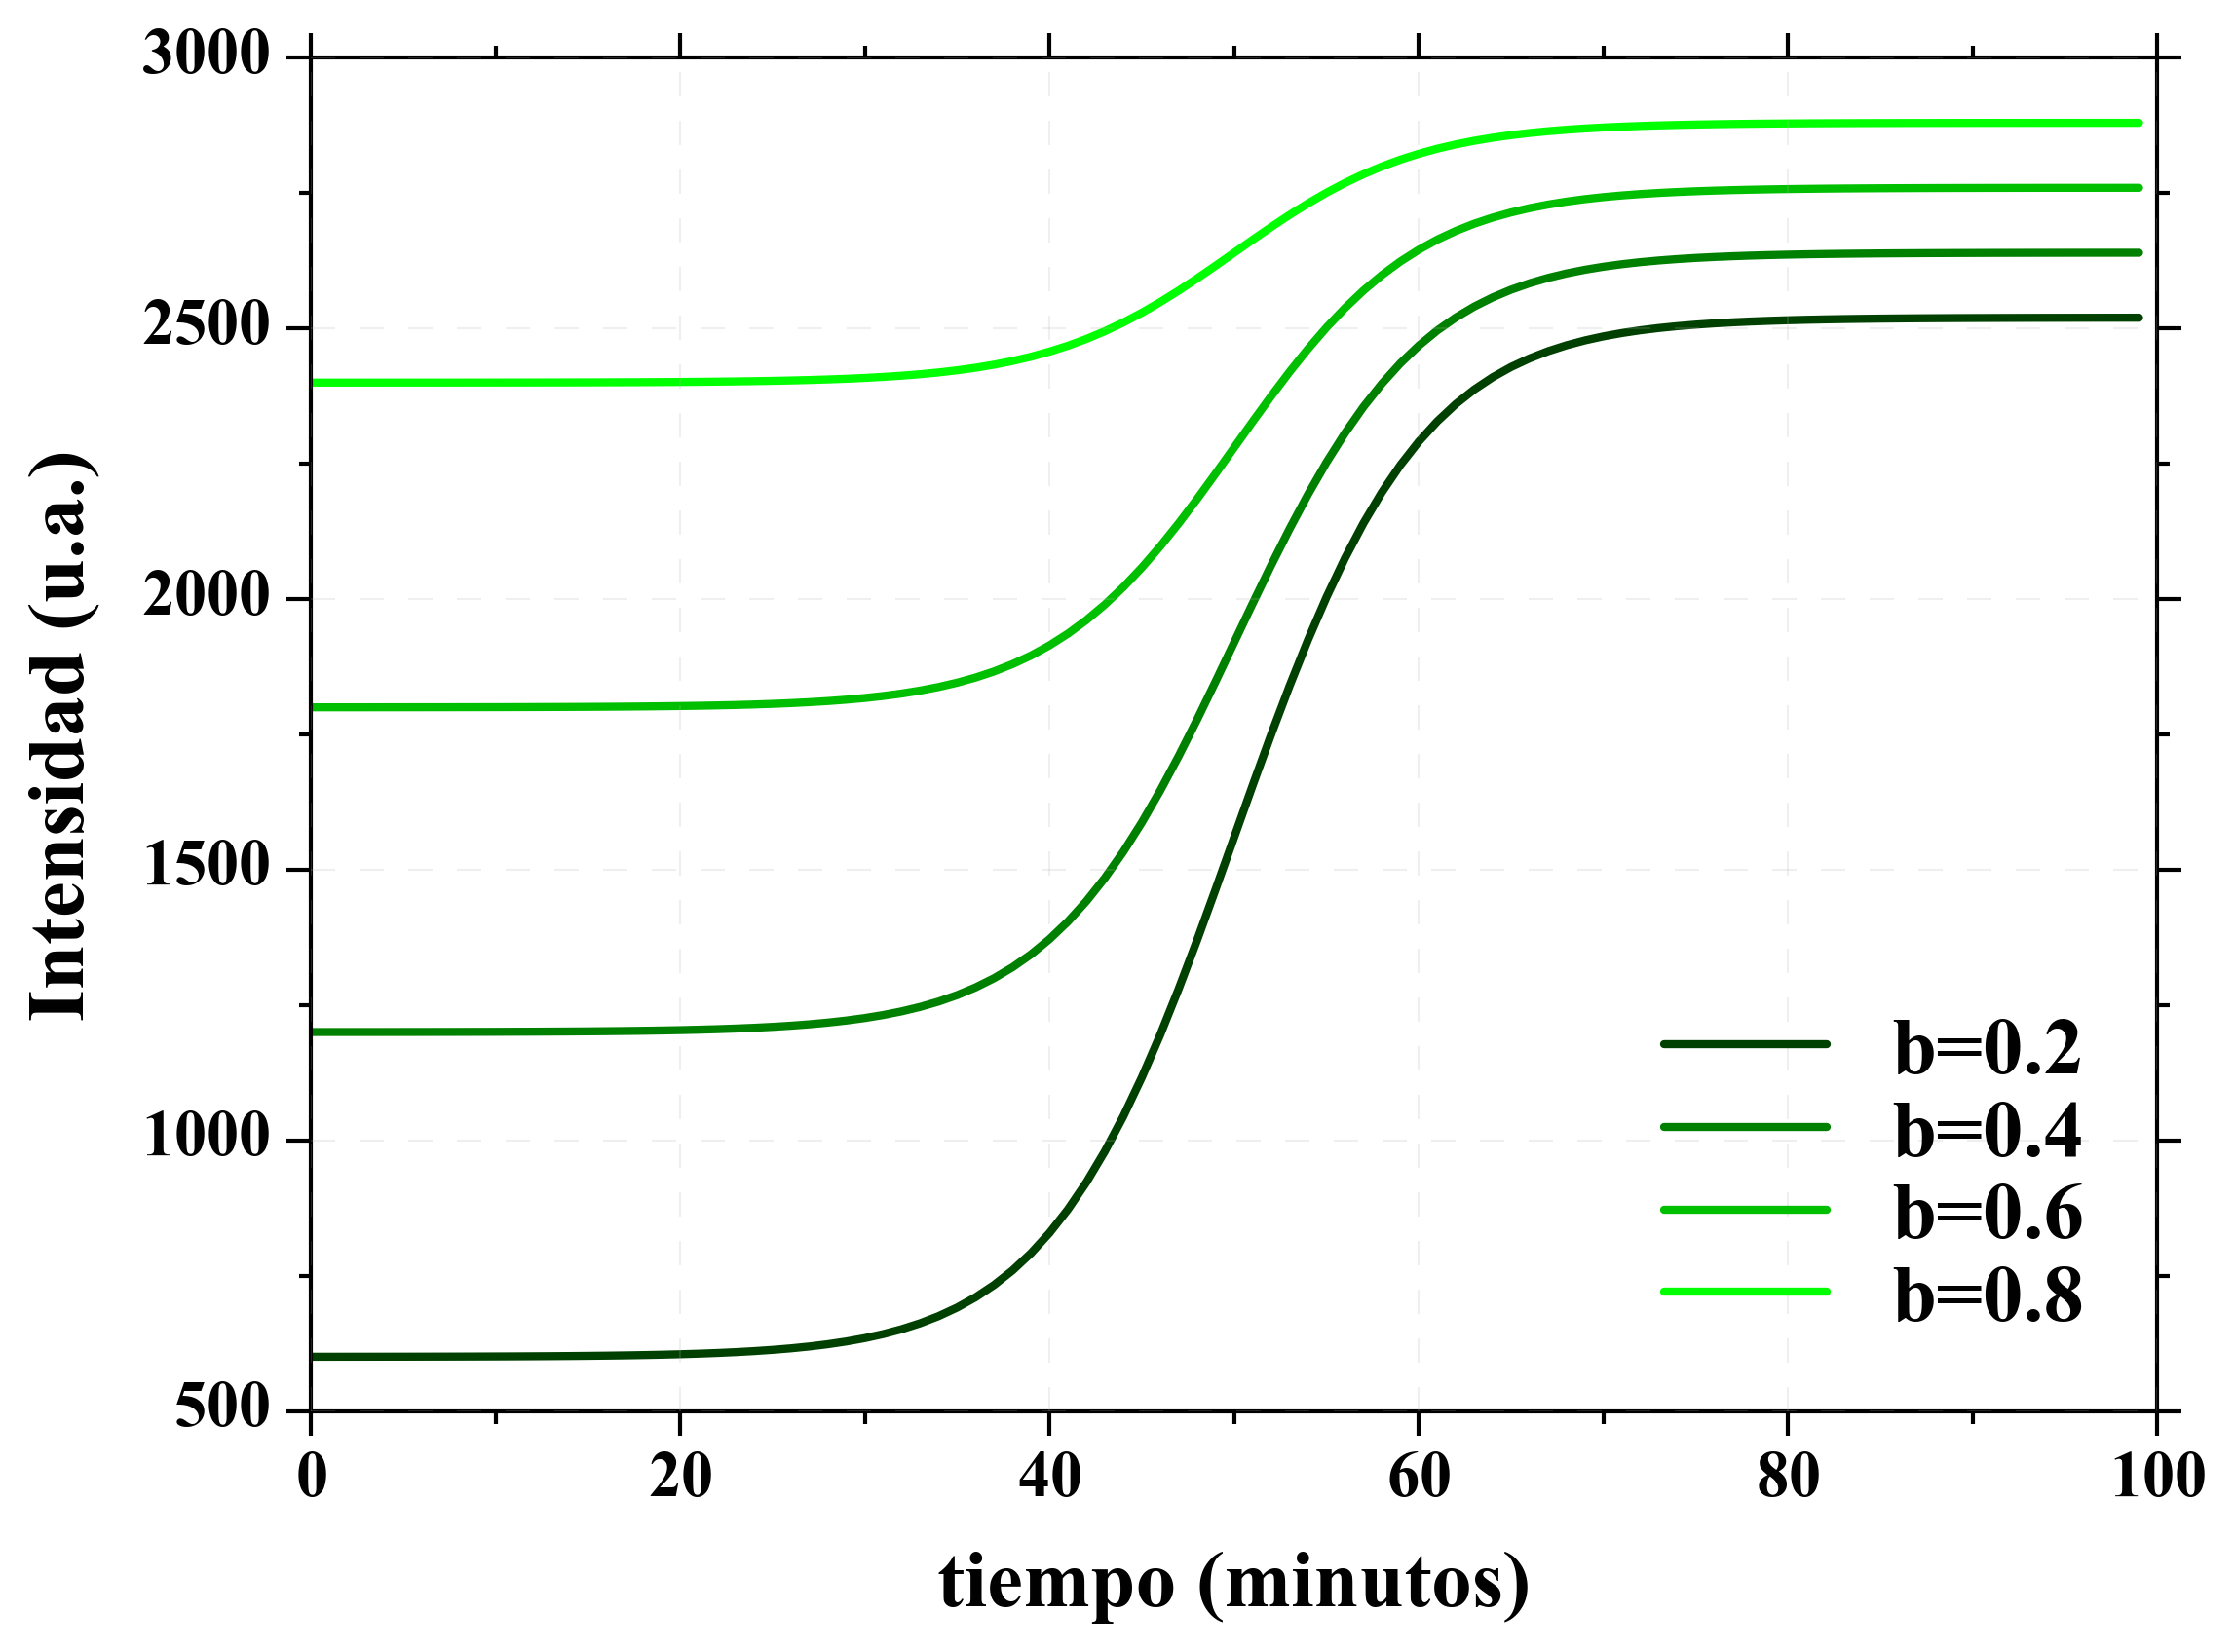
\includegraphics[width=0.6\textwidth]{./img/f_sim.png}
    \caption{Curva de intensidad total de fluorescencia generada a partir de la curva simulada para $m$. Se utilizaron $b_M C = 3000$, mientras que para el valor de $b$ se realizó un barrido entre $0.2$ y $0.8$.}
    \label{fig:f_sim}
\end{figure}

En la figura \ref{fig:f_sim} pueden destacarse algunas características clave de los parámetros. En primer lugar, y como se mencionó previamente, $C b_M$ sirve como parámetro de escala para la intensidad total. Por otro lado, considerando que $b$ muestra la relación entre los brillos de ambos estados del sensor, no nos debe sorprender que cuanto más se aleje de la unidad, mayor será la variación de intensidad de fluorescencia. Además, los distintos valores de $b$ producen distintos valores iniciales y finales de intensidad total. Este hecho sería distinto si el clivaje del sensor fuese del $100\%$.

Podemos apreciar que la anisotropía y la intensidad total de fluorescencia representan un cambio de variables de los observables experimentales que son $I_{\parallel}$ e $I_{\perp}$ a través de la ecuación \ref{eq:anisotropia} y su denominador $I_T = I_{\parallel} +2 I_{\perp}$. Entonces, es posible trabajar sobre cualquiera de las dos, o alguna combinación, para obtener información sobre los parámetros importantes y el estado del ensamble de fluoróforos. Utilizando las relaciones mencionadas, podemos despejar $I_{\parallel}$ e $I_{\perp}$ en función de los parámetros buscados

\begin{align}
    I_{\parallel} &= (\alpha_{\parallel} m + \beta_{\parallel}) \frac{2}{3}Cb_M \label{eq:Int_par}\\
    I_{\perp} &= (\alpha_{\perp} m + \beta_{\perp}) \frac{1}{3} Cb_M,\label{eq:Int_per}
\end{align}

\noindent donde

\begin{multicols}{1}

\begin{align}
    \alpha_{\parallel} & = (r_M + 1/2) - (r_D + 1/2) b\\
    \alpha_{\perp}     & = (1 - r_M) - (1 - r_D) b
\end{align}

\begin{align}
    \beta{\parallel}   & = (r_D + 1/2) b\\
    \beta{\perp}       & = (1 - r_D) b.
\end{align}

\end{multicols}

Habiendo hallado las expresiones matemáticas que describen a $I_{\parallel}$ e $I_{\perp}$ en función de los parámetros y el estado del ensamble, podemos graficar las curvas correspondientes a estas intensidades a partir de la simulación realizada. Dichos gráficos se presentan en la figura \ref{fig:Ints_sim}.

\begin{figure}
\centering
    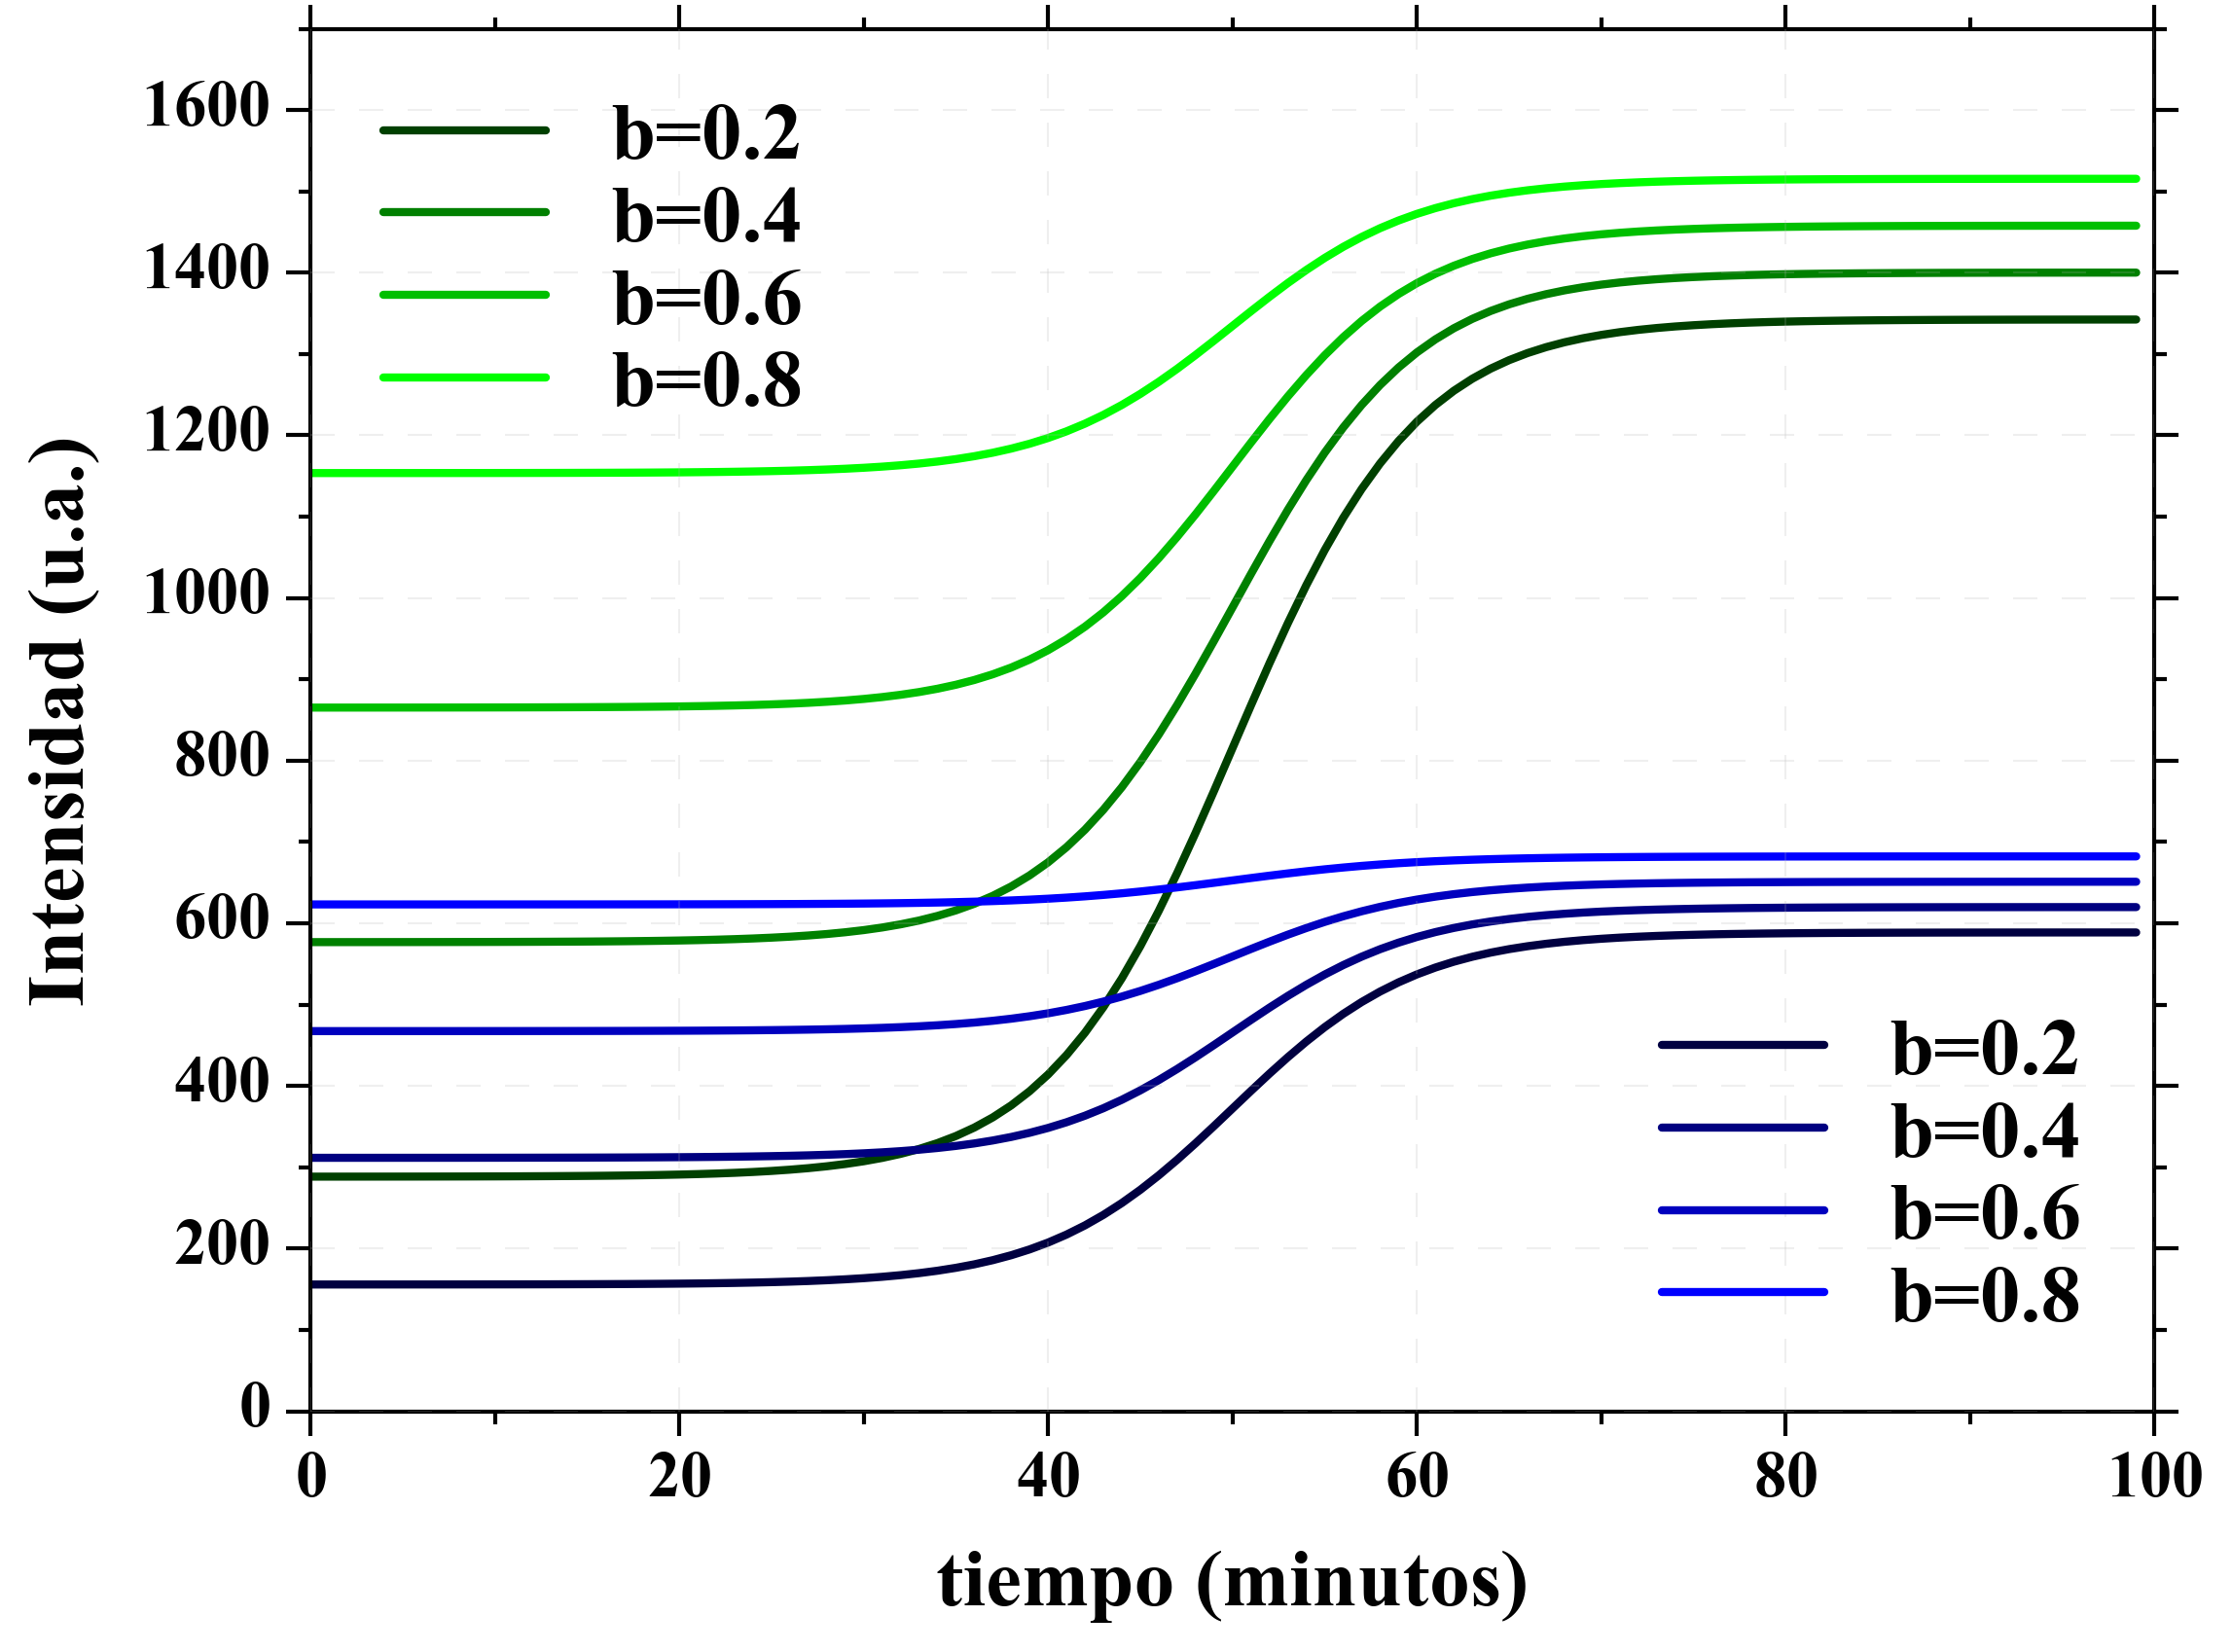
\includegraphics[width=0.6\textwidth]{./img/Ints_sim.png}
    \caption{Curvas de $I_{\parallel}$ e $I_{\perp}$ generadas a partir de la curva simulada para $m$. Se utilizaron los parámetros definidos previamente, a saber, $b_M C = 3000$, $r_D=0.221$ y $r_M=0.303$, mientras que para el valor de $b$ se realizó un barrido entre $0.2$ y $0.8$.}
    \label{fig:Ints_sim}
\end{figure}


%%%%%%%%%%%%%%%%%%%%%%%%%%%%%%%%%%%
\section{Transformación de los Observables Fotofísicos}

A continuación, podemos utilizar las expresiones matemáticas despejadas para transformar los datos simulados y probar así la validez de estos métodos para recuperar información sobre el estado del ensamble de fluoróforos, así como también sus parámetros característicos. En nuestro experimento mental, teníamos una cubeta con un único tipo de sensor cuya cantidad de fluoróforo se mantenía constante a lo largo del experimento, hecho que se refleja en un valor de $C$ constante. Además, los valores de $r_D$, $r_M$, $b_M$ y $b_D$ son específicos para cada fluoróforo, razón por la cual también deben considerarse globales para esta curva. A diferencia de estos parámetros, la proporción de fluróforos en estado monomérico, $m$, puede tomar un valor distinto para cada instante. Aunque esto implicaría que por cada punto agregado, hay un parámetro adicional para ajustar, se debe notar que también se agregan dos observables experimentales medidos, $I_{\parallel}$ e $I_{\perp}$. Si tenemos en cuenta los 4 parámetros globales ($r_D$, $r_M$, $b$ y $C b_M$) y cada $m$ por cada punto, apreciamos que se necesitan al menos cuatro puntos para poder hallar una solución para el sistema. Es esencial notar que $r_D$, $r_M$, $b$ siguen siendo específicos del fluoróforo utilizado, pero $C b_M$ depende de la cubeta analizada ya que cada cubeta puede tener concentraciones distintas.

Con el objetivo de diseñar y validar el método de ajuste para recuperar los parámetros buscados, se programaron en \textit{Python} (\textit{v. 3.4.4}) los algoritmos necesarios para hallar el mínimo de la función de $\chi ^2$. Esta consiste en minimizar

\begin{equation}
    \chi ^2 = \sum \frac{(Observado - Esperado)^2}{Varianza},
\end{equation}

\noindent donde el $Observado$ y la $Varianza$ se refieren a los valores observados experimentalmente mientras que el $Esperado$ corresponde al valor predicho por la teoría. Luego, los parámetros son ajustados para que la curva teórica se asemeje lo más posible a la observada. %En este caso, se utilizaron las ecuaciones \ref{eq:Int_par} y \ref{eq:Int_per} para ajustar las curvas simuladas.

Previo a proceder con los distintos métodos de transformación, discutamos como evaluaremos una buena transformación. Antes que nada, esta claro que debe minimizar $\chi ^2$ de las curvas ajustadas. En segundo lugar, se evaluará si describe adecuadamente la anisotropía observada mediante el cálculo de la suma de todas las diferencias al cuadrado entre los puntos observados y los ajustados. Además, los parámetros utilizados para generar la curva deberían ser recuperables a partir del ajuste, incluso en presencia de ruido blanco. Esta claro, que si la anisotropía es transformada correctamente, el ruido proveniente de su medición también será observado en las curvas de $m$ obtenidas. Esta fidelidad de la transformación con los datos experimentales permite desentenedrnos de las observaciones experimentales y trabajar con la curva de $m$ como si fuese nuestro observable experimental. %Por último, considerando que nuestro objetivo es obtener información confiable del estado del ensamble de fluoróforos, 


%Previo a proceder con los distintos métodos de ajuste mencionados, discutamos como evaluaremos un buen ajuste. Antes que nada, esta claro que debe minimizar $\chi ^2$ de las curvas ajustadas. En segundo lugar, se evaluará si también describe adecuadamente las curvas que no fueron ajustadas pero se deducen a partir del ajuste. Además, los parámetros utilizados para generar la curva deberían ser recuperables a partir del ajuste, incluso en presencia de ruido blanco. Por último, considerando que nuestro objetivo es obtener información confiable del estado del ensamble de fluoróforos, calcularemos el valor de $\chi ^2$ para la curva de $m$ obtenida, así como también $m$ normalizada.

%Por último, introduciremos un parámetro nuevo que cobrará sentido en el próximo capítulo y es importante que sea ajustado correctamente. Este consiste en calcular el máximo de la derivada temporal de $m$ dividido por $d$ (siendo $d=D/C$), al cual denominaremos $\Delta m/d$. Sin entrar en detalles, dicho parámetro nos da una idea de la actividad enzimática y su máximo determina el máximo de actividad.

%\todo{deberia ser $\Delta m$ pero tal vez no haga falta analizarlo}

Habiendo introducido todos los conceptos necesarios para ajustar la transformación de las curvas experimentales, procedemos a evaluar si los parámetros de las curvas simuladas pueden ser recuperados adecuadamente. Simultáneamente, se analizará si el resto de las curvas son recuperadas adecuadamente a partir de las ajustadas. En principio, y siguiendo con el método descripto usualmente en la bibliografía, se ajustará la anisotropía. Dado que son necesarios dos observables para ajustar como se explicó previamente, también utilizaremos la intensidad total observada.

Con el objetivo de introducir ruido en las mediciones de la misma forma que se vería experimentalmente, se confeccionaron funciones que toman las curvas de intensidades cruzadas simuladas y le agregan ruido gaussiano a cada punto. Luego, se recalculaban las curvas de anisotropía e intensidad total a partir de las curvas con ruido agregado. Esto se hizo de esta forma ya que el observable experimental directo son las intensidades cruzadas, y la propagación a anisotropía e intensidad total del ruido no es lineal. Para estas simulaciones se utilizaron las curvas con $b=0.6$.

Ajustar las curvas de anisotropía e intensidad total simuladas mediante las ecuaciones \ref{eq:AnisotropiaFromParams} y \ref{eq:Int_fromFit} dieron muy buenos resultados, como se puede apreciar en la figura \ref{fig:fit_AnNoisy}.

\begin{figure}
\centering
    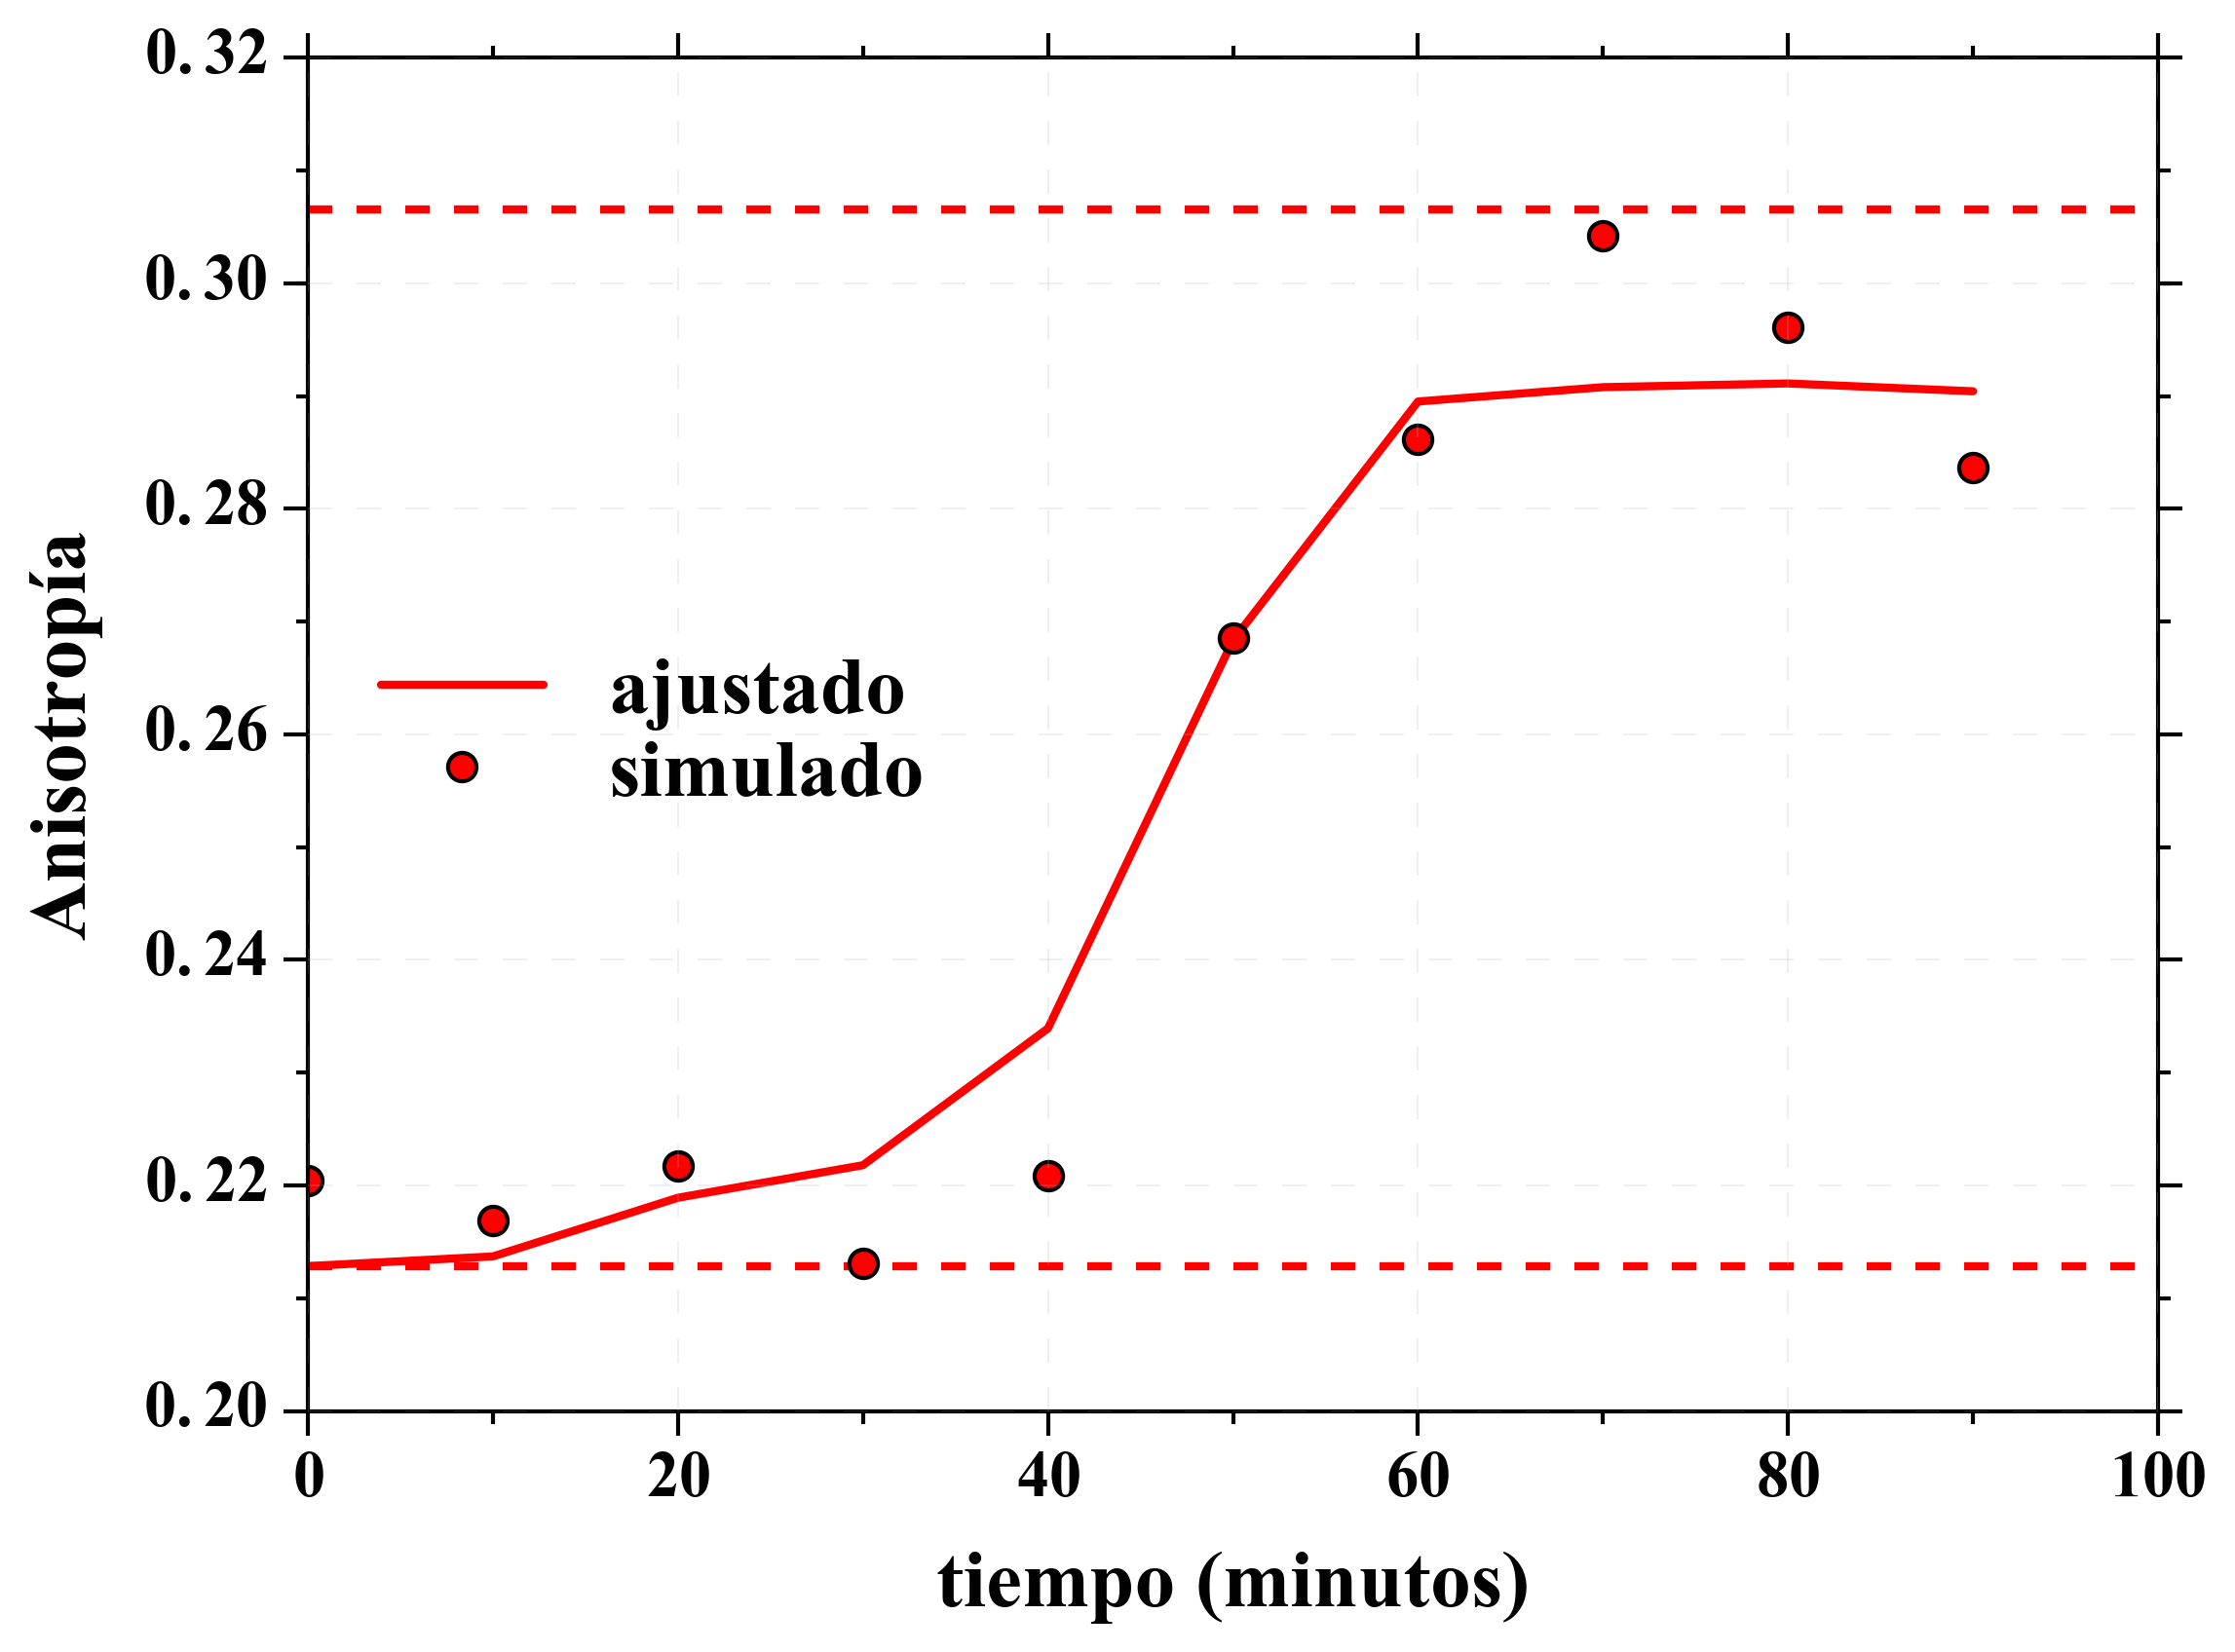
\includegraphics[width=0.5\textwidth]{./img/An_Fit.png}
    \caption{Ajuste de la anisotropía y la intensidad total mediante las ecuaciones \ref{eq:AnisotropiaFromParams} y \ref{eq:Int_fromFit}. Puede apreciarse que el ajuste no recupera de manera fiel los valores de anisotropía, pero promedia el ruido agregado.}
    \label{fig:fit_AnNoisy}
\end{figure}

Dado que experimentalmente se observan $I_{\parallel}$ e y $I_{\perp}$, es buena práctica trabajar directamente con estos observables para evitar propagar sus errores a anisotropía. Se procedió a ajustar dichas curvas simuladas utilizando las ecuaciones \ref{eq:Int_par} y \ref{eq:Int_per}. En la imagen \ref{fig:fit_Icrossed} se presenta un ejemplo de dicho ajuste.

\begin{figure}
\centering
    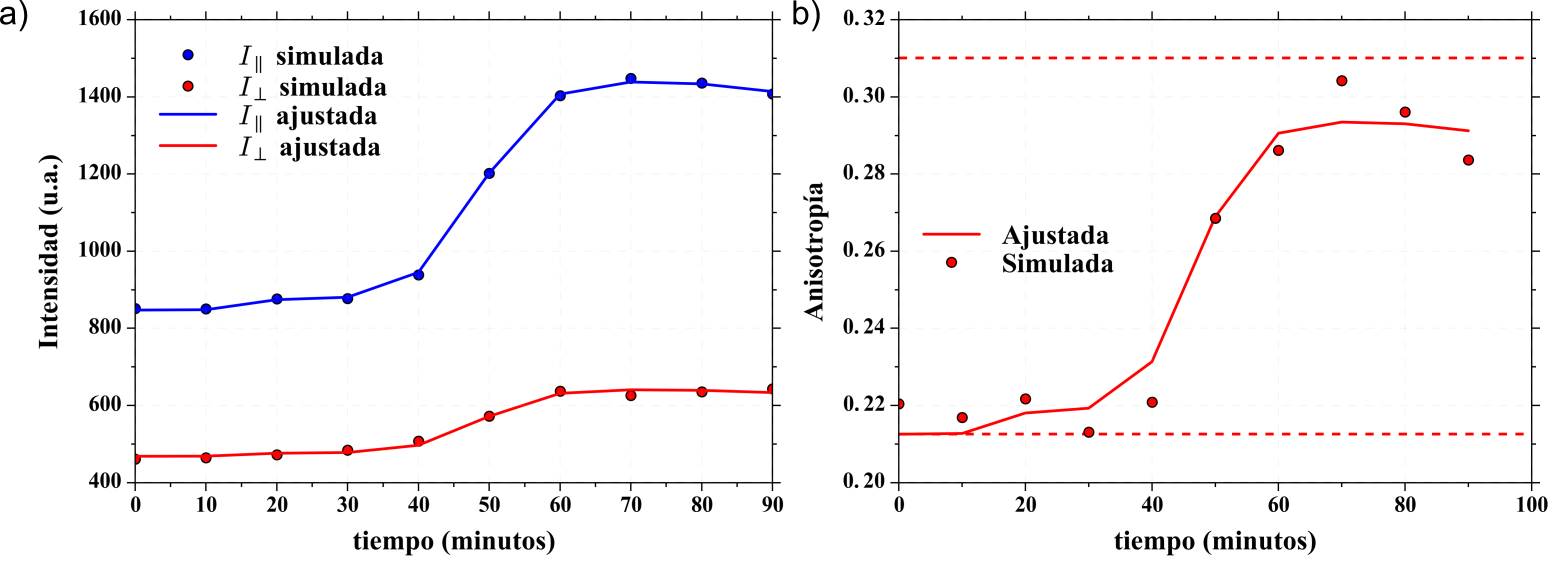
\includegraphics[width=0.9\textwidth]{./img/AjusteInts.png}
    \caption{Ajuste de las intensidades cruzadas mediante las ecuaciones \ref{eq:Int_par} y \ref{eq:Int_per}. \textbf{a)} Gráfico de las intensidades cruzadas ajustadas (trazo continuo) y los datos simulados (círculos). \textbf{b)} Gráfico de la anisotropía ajustada (trazo continuo) superpuesto con los datos simulados de anisotropía (círculos). Puede apreciarse que el ajuste no recupera de manera fiel los valores de anisotropía, pero promedia el ruido agregado.}
    \label{fig:fit_Icrossed}
\end{figure}

Por último, considerando que no se necesita conocer el parámetro de escala se procedió a ajustar las curvas correspondientes a las intensidades cruzadas normalizadas por la intensidad total. Este ajuste tiene la particularidad de que $C b_M$ se cancela en las expresiones a ajustar. Se presenta en la figura \ref{fig:Int_r_Fit} las curvas correspondientes al ajuste y la curva de anisotropía obtenida a partir de este.

\begin{figure}
\centering
    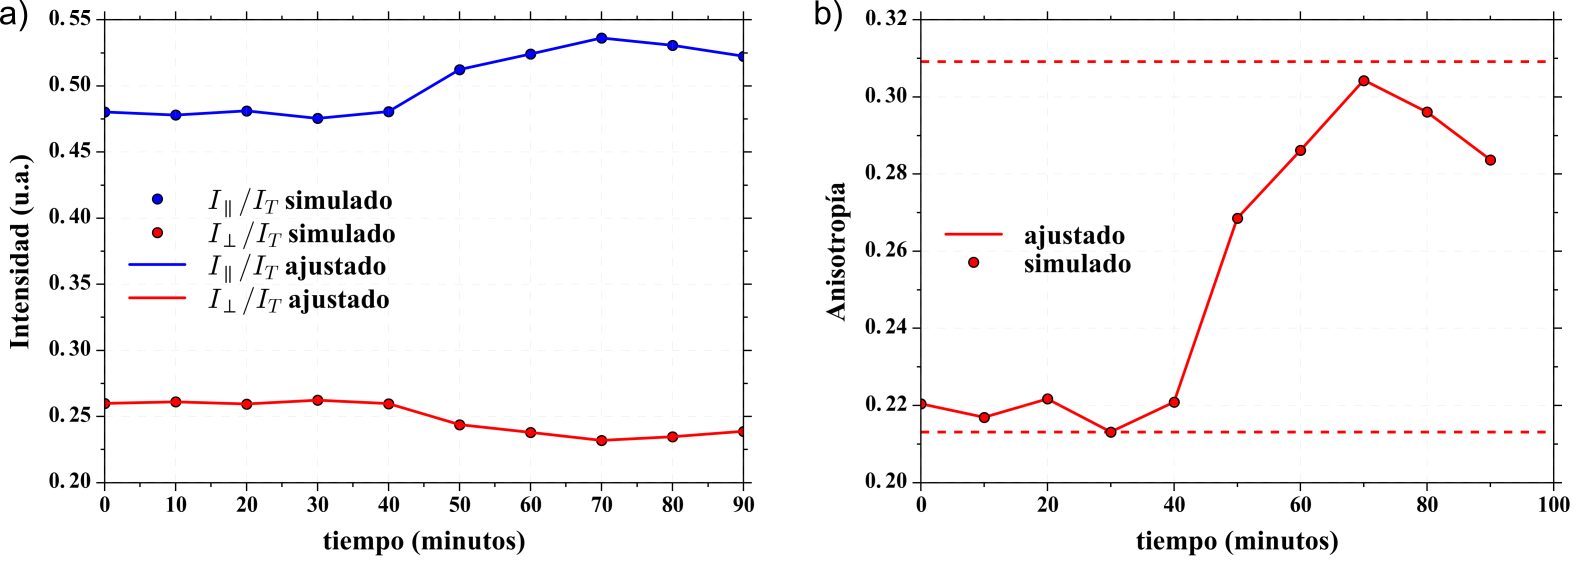
\includegraphics[width=0.9\textwidth]{./img/Ajuste_Int_r.png}
    \caption{Ajuste de las intensidades cruzadas normalizadas. \textbf{a)} Se graficaron las curvas correspondientesa los ajustes de las intensidades cruzadas normalizadas superpuestas con los datos experimentales. \textbf{b)} Se graficó la curva de anisotropía obtenida a partir del ajuste superpuesta con los datos experimentales. Puede apreciarse que el ajuste recupera de manera fiel los valores de anisotropía.}
    \label{fig:Int_r_Fit}
\end{figure}

Habiendo ajustado todas las curvas simuladas, podemos analizar que tan bien fueron reproducidos los parámetros del ajuste. En la figura \ref{fig:fit_Params} se presentan gráficos de los valores recuperados para los parámetros utilizando los distintos métodos. Puede apreciarse una elevada similitud entre ajustar la anisotropía y la intensidad total o las intensidades cruzadas. Por otro lado, la mayor diferencia radica en ajustar las intensidades cruzadas normalizadas. Se debe destacar que este último método no siempre devuelve los parámetros correctamente ajustados.

\begin{figure}
\centering
    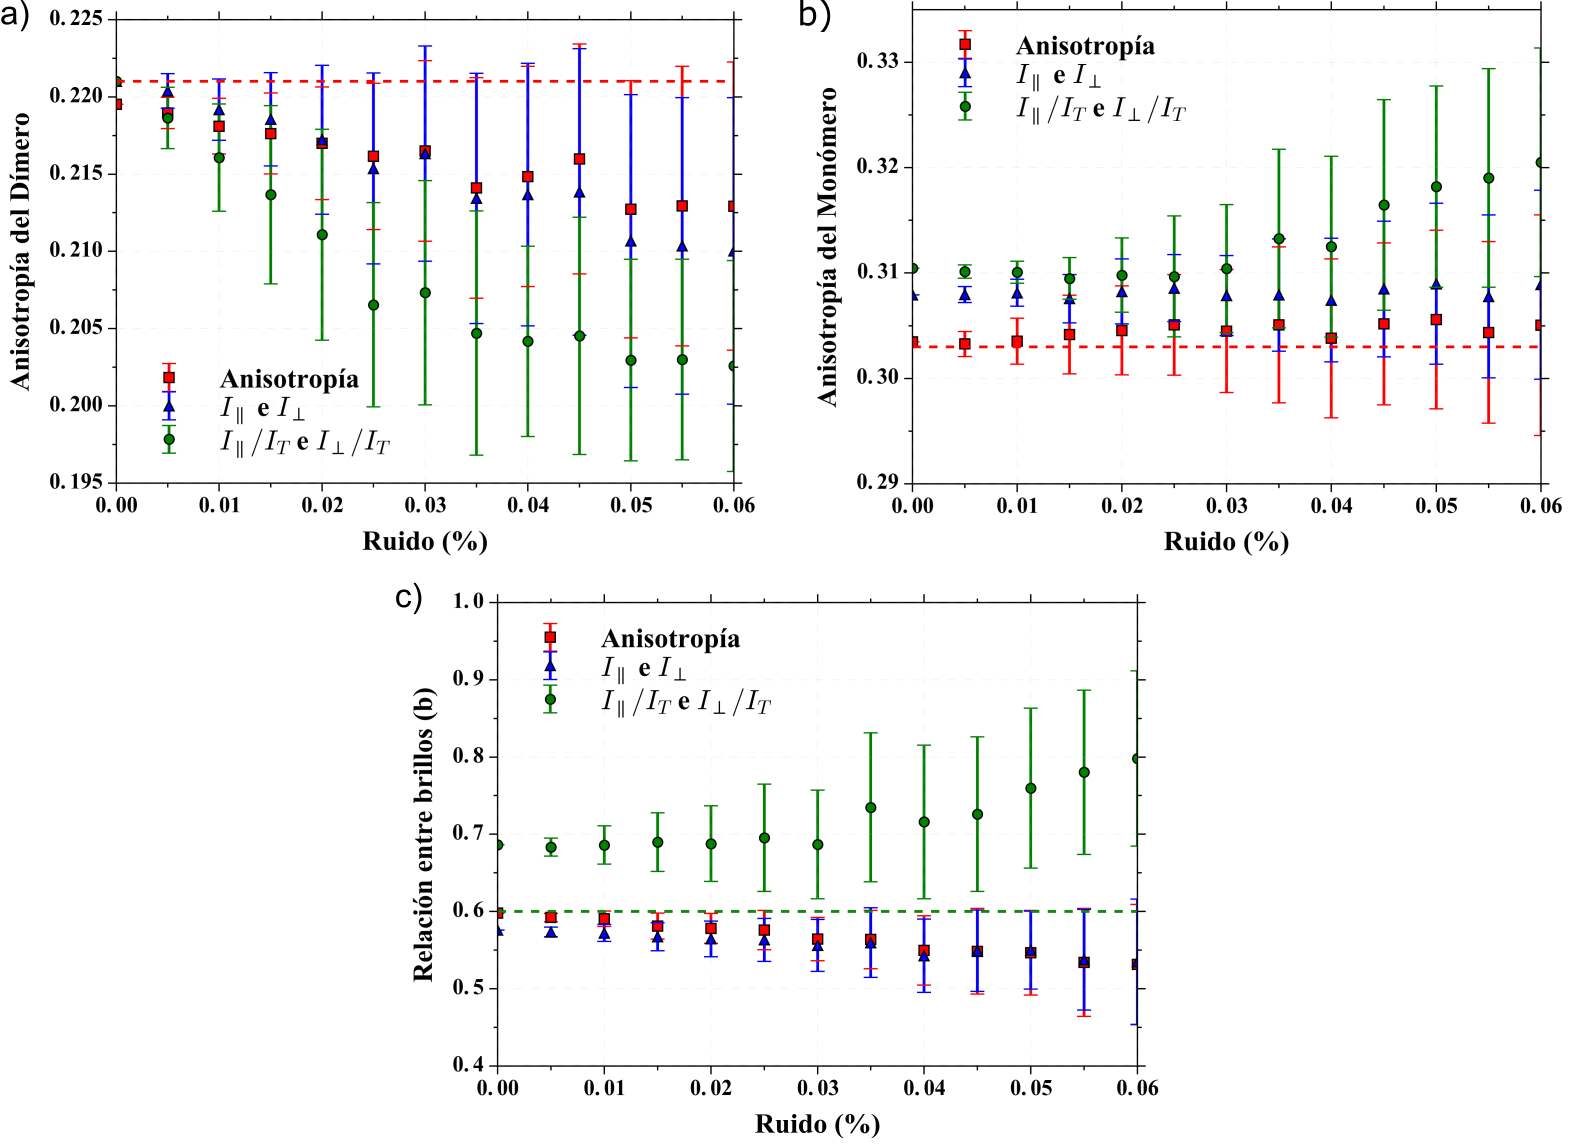
\includegraphics[width=0.9\textwidth]{./img/Ajustes_Params.png}
    \caption{Análisis de parámetros obtenidos a partir de los distintos ajustes. \textbf{a)} Se presentan los valores obtenidos para la anisotropía del Dímero. \textbf{b)} Se presentan los valores obtenidos para la anisotropía del Monómero. \textbf{c)} Se presentan los valores obtenidos para la relación entre intensidades.}
    \label{fig:fit_Params}
\end{figure}

Por otro lado, si observamos la semejanza entre las curvas de anisotropía obtenidas a partir de los parámetros ajustados y la anisotropía generada a partir de la simulación con ruido, podemos apreciar que ajustando las curvas de intensidades cruzadas normalizadas es considerablemente más preciso. En la figura \ref{fig:Ajuste_chi_a} se presenta un gráfico de la suma cuadrática de la diferencia entre los puntos estimados y los simulados para mostrar la afirmación. 
\begin{figure}
\centering
    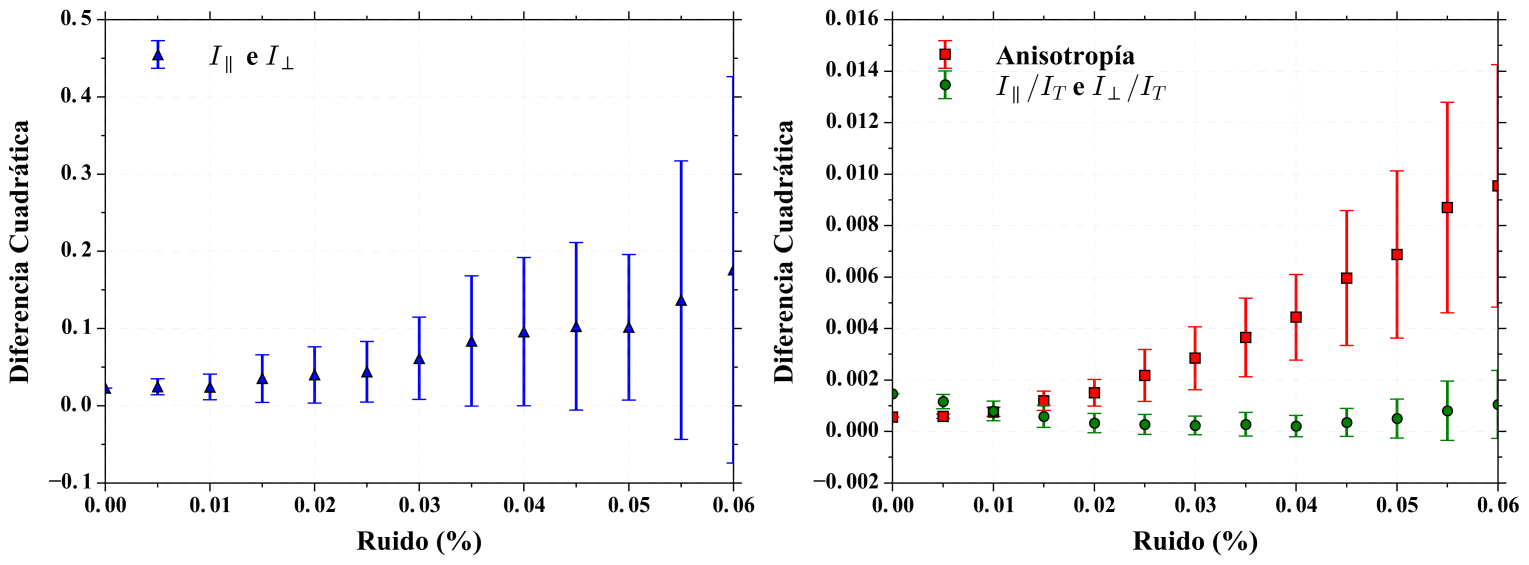
\includegraphics[width=0.9\textwidth]{./img/Ajuste_chi_a.png}
    \caption{Gráfico de la suma cuadrática de la diferencia entre los puntos simulados y los obtenidos a partir del ajuste de los parámetros para la anisotropía. Se graficaron por separado para apreciar la diferencia en orden de magnitud.}
    \label{fig:Ajuste_chi_a}
\end{figure}

A partir de estos análisis se deduce que el ajuste de las intensidades cruzadas normalizadas es fiel al ajuste de la anisotropía, incluso cuando no es el mejor método para obtener el valor de los parámetros. Esto último nos conduce a pensar que ajustar las intensidades cruzadas normalizadas transforma de manera fiel los observables fotofísicos en una curva de proporción de sensor en estado monomérico (ver figura \ref{fig:todos_ms}). De esta forma, uno puede transformar los observables experimentales mediante este método y puede asegurarse que toda la información se verá plasmada en una curva que describe el estado del ensamble de fluoróforos con el mismo ruido que la curva observada experimentalmente. Simultáneamente, este método presenta una mejora teórica al cancelar el parámetro de escala, que varía con cada cubeta.

\begin{figure}
\centering
    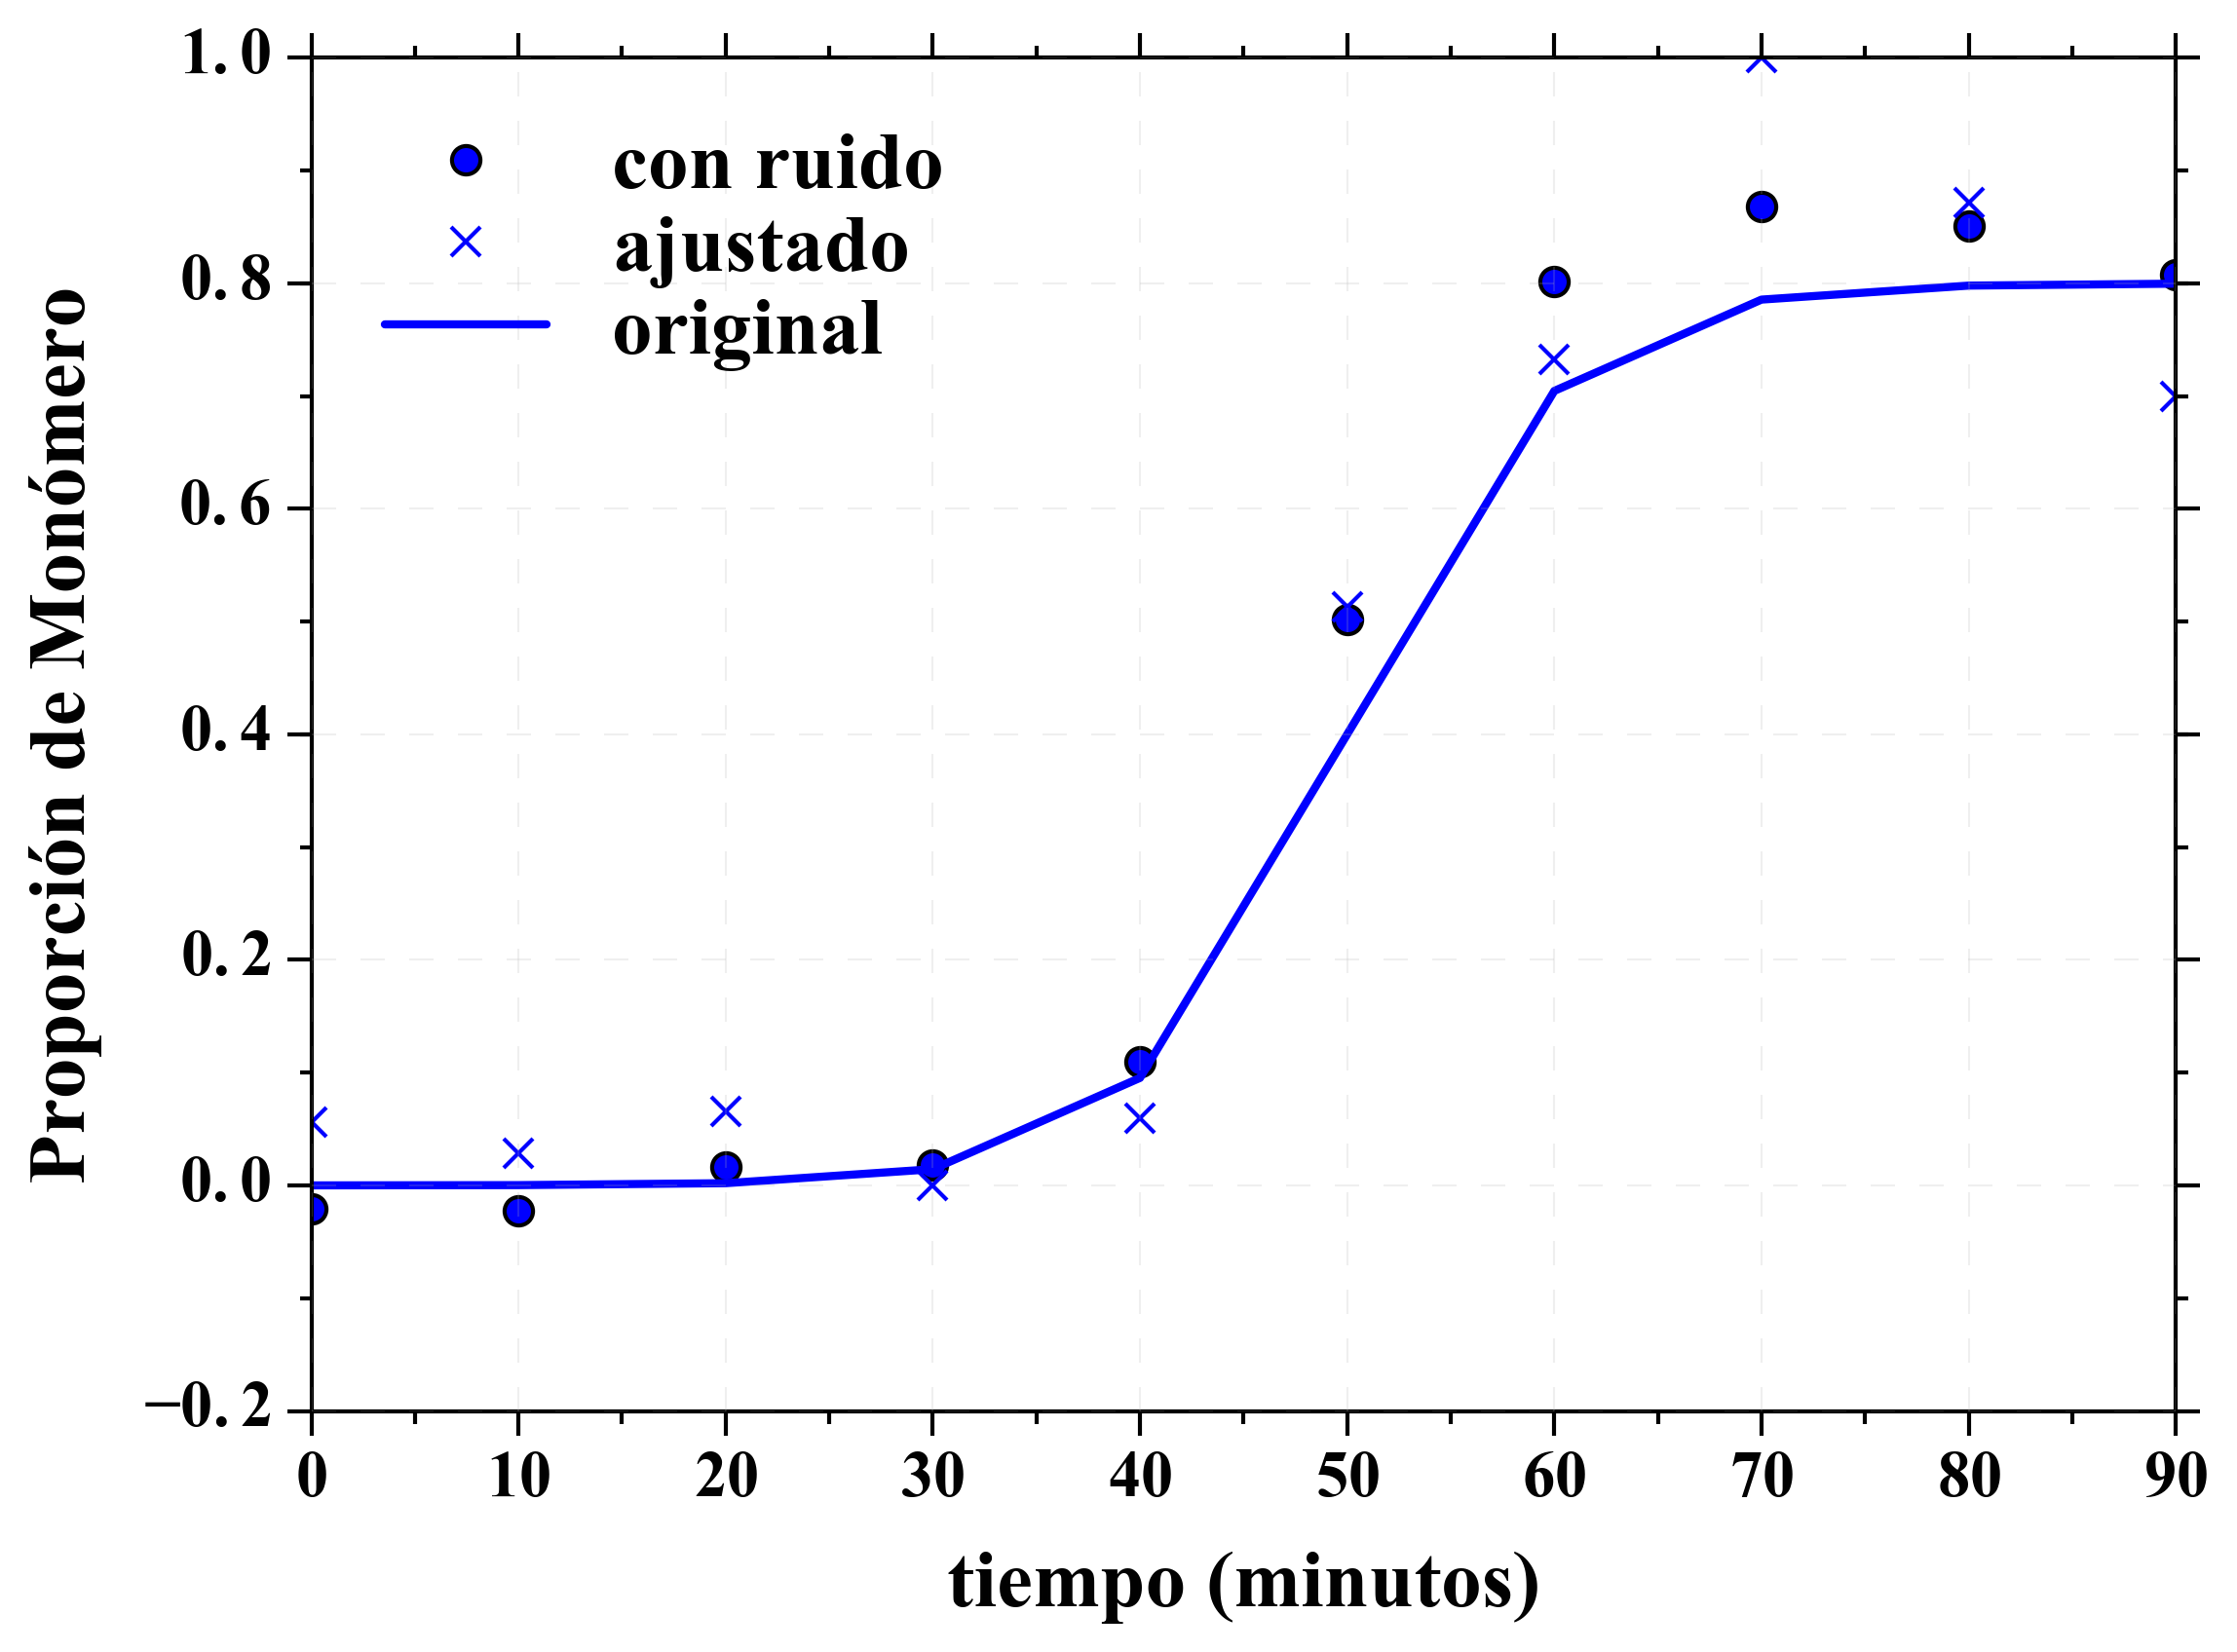
\includegraphics[width=0.5\textwidth]{./img/todos_ms.png}
    \caption{Se superpusieron los gráficos de la curva de proporción de fluoróforo simulada originalmente con sus versiones simuladas con ruido de 3$\%$ y su ajuste. Puede apreciarse una elevada similitud entre los valores obtenidos del ajuste y su contraparte simulada con ruido.}
    \label{fig:todos_ms}
\end{figure}

 %En los casos ideales, este ajuste es capaz de reproducir fielmente los parámetros introducidos, mientras que en la figura \ref{fig:chis} se presenta el corrimiento de $\chi ^2$ a medida que aumenta el ruido en las curvas analizadas.

%En la figura \ref{chis} se presenta una superposición de los valores de $\chi ^2$ obtenidos con cada método de ajuste. Puede apreciarse la ventaja que ajustar las intensidades cruzadas tiene sobre ajustar la anisotropía y la intensidad total. Por lo que se concluye que ajustar sobre los observables experimentales es más robusto que trabajar sobre la señal de anisotropía e intensidad total que se calculan a partir de los observables.


%\todo{Esto es viejo}

%De todas formas, este método produjo resultados pobres al aplicarse a los datos experimentales. Esto se debe principalmente al origen de ruido subyacente en los datos experimentales.

%En la figura \ref{fig:fit_ICrossed_exp} se presenta el ajuste sobre las curvas de intensidades cruzadas y la curva de anisotropía que surgen de los parámetros obtenidos mediante el ajuste. Puede apreciarse una diferencia importante entre la anisotropía obtenida experimentalmente y la correspondiente al ajuste. Esta incongruencia puede explicarse si se tiene en cuenta la propagación de errores al momento de traducir las intensidades cruzadas en anisotropía. Los errores relativos al realizar este pasaje son aumentados al menos en un orden de magnitud, disminuyendo considerablemente el valor de este método.

%\todo{la idea de la propagacion se puede pulir un poco mas}

%\todo{Aca iria la img de ajuste de int cruzadas experimental con la anisotropia obtenida}

%Al analizar la fuente del error en el ajuste, apreciamos que los errores se ven amplificados cuando observamos la curva de anisotropía obtenida. En segundo lugar, variaciones en la máscara generada para segmentar la imagen a analizar nos genera curvas de intensidades cruzadas complicadas de ajustar. Sin embargo, si normalizamos las intensidades obtenidas respecto de la intensidad total podemos, no solo desentendernos del parámetro de escala, sino que las curvas de intensidades cruzadas normalizadas resultan más suaves al despreciar cualquier defecto en la segmentación de imágenes.

%Se repitieron los estudios realizados sobre el método para ajustar intensidades cruzadas y se observó que, aunque los parámetros no podían ser reproducidos adecuadamente, era posible obtener la curva normalizada de proporción de fluoróforo en estado monomérico y sus parámetros de tiempo de máxima actividad.

%En la imagen \ref{fig:fit_ICrossed_N_exp} se presenta un ajuste sobre las curvas de intensidades cruzadas normalizadas y la curva de anisotropía que se obtiene a partir de los parámetros ajustados. Puede apreciarse que la fidelidad entre ambas curvas de anisotropía es mayor que cuando se ajustaban las curvas de intensidades cruzadas sin normalizar. De esta forma, mostramos que ajustando las intensidades cruzadas normalizadas obtenemos una representación más fiel de la proporción de fluoróforo en estado monomérico.

%Si prestamos especial atención a la forma de la curva, podemos apreciar que la anisotropía calculada se asemeja a la intensidad ajustada, hecho que genera una curva de anisotropía poco fiel.

%\todo{Aca iria la img de ajuste de int cruzadas normalizado experimental con la anisotropia obtenida}

%\todo{Esto es mas viejo}

%En realidad hay 3 casos: ajustar anisotropía y fluorescencia total (no lo hice, aunque lo probé con los datos y no andaba), ajustar $I_{\parallel}$ e $I_{\perp}$ (esta hecho y parece andar bien todo en simulada con ruido, pero fallaba con datos) y, por último, las intensidades cruzadas normalizadas (que parecían andar en todos los casos, excepto a la hora de recuperar $b$ en las simuladas).

%Pensaba presentar las dos de intensidades cruzadas, pero tengo muchas cosas para comparar y mostrar. Lo más importante para mí es mostrar que describe bien intensidades cruzadas y anisotropía. Pero después puedo mostrar por cuanto le erra a cada parámetro (gráficos). Y ni hablar de ir variando la proporción inicial y final a la que llega. Todo esto con el método que me dijiste la última vez de dejar libre las anisotropías en el rango que veo experimental, después estaba la posibilidad de fijarlo en cada curva al que mido ahí.

%Para simular el ruido, lo que hacía era meterlo en la anisotropía y la fluorescencia total.

%Ajustar intensidades cruzadas parece devolver mejor el parámetro b. Pero cdo vamos a los datos este método no va bien.


%%%%%%%%%  Modelado
\chapter{Modelo de Red de Caspasas}
\label{cap:modelo}

Actualmente, en biología de sistemas se utilizan los modelos matemáticos de bioquímica con el objetivo de modelar redes de proteínas y reacciones que ocurren \ening{in vivo}. Es así que se utilizan redes de ecuaciones diferenciales ordinarias que surgen de la ley de acción de masas\cite{Chen2010}. Estos modelos son validados mediante contraste experimental y poseen valor predictivo a la hora de estudiar un sistema o diseñar nuevos experimentos.

%sirven, también, para explicar la aproximación de Michaelis Menten. En este caso, las ecuaciones diferenciales ordinarias

Es de conocimiento general los modelos de Michaelis y Menten (1913) desarrollados hace aproximadamente un siglo para comprender la dinámica enzimática. Este a su vez se basaba en los hallazgos de Haldi (1902) y fue clarificado posteriormente por Briggs y Haldane (1925) una década después. Luego fueron extendidos en las décadas subsiguientes por Monod et. al (1965), Koshland (1966) y Goldbeter y Koshland (1981). Estos modelos se concentran en describir reacciones enzimáticas controladas \ening{in vitro} y en condiciones de concentraciones homogéneas\cite{Chen2010}. Extensiones de los mismos son utilizadas para modelar cascadas de señalización más complejas en las células.


%%%%%%%%%%%%%%%%%%%%%%%%%%%%%%%%%%%%%%%%%%%%%%%%%%%
\section{Ley de acción de masas}

La ley fundamental de una reacción química es la de acción de masas. Esta describe la tasa a la cual los elementos químicos, sean tanto macromoléculas o simples iones, colisionan e interactúan para formar los distintos productos. Comencemos por considerar una reacción simple en la que los sustratos $A$ y $B$ colisionan para formar $C$, es decir,

\begin{center}
\ce{A + B ->[k] C,}
\end{center}

\noindent donde $k$ se denomina la constante de reacción. Esta surge de considerar que las colisiones de las moléculas en el sistema en equilibrio térmico se dan de forma completamente aleatoria. Esta constante depende a su vez de la relación entre los tamaños de las especies involucradas, su geometría y otros parámetros que pueden reducirse a la probabilidad de encuentro y reacción exitosa\cite{Gillespie1977}.

Asumiendo que la concentración de las especies en estudio pueden ser descriptas mediante funciones continuas, y que cada una de sus reacciones químicas pueden representarse como procesos continuos, es posible construir una serie de ecuaciones diferenciales acopladas que describan la dinámica. En este caso particular, la variación de la concentración del producto ($C$) que descripta por\cite{Gillespie1977}

\begin{equation}
    \frac{dC}{dt} = k[A][B],
\end{equation}

\noindent donde $[A]$ y $[B]$ se refieren a las concentraciones de $A$ y $B$ respectivamente. Al igual que la ley de Ohm o la ley de Newton para enfriamiento, esta tiene cierto rango de validez. En primer lugar, si se trabaja a concentraciones altas, duplicar la concentración no implica que necesariamente se duplique la tasa de formación de producto. En el otro extremo, si se utilizan concentraciones muy bajas, puede que representar la concentración como una variable continua no sea la mejor opción\cite{Keener1998}.

A continuación, si deseamos estudiar que sucede con reacciones reversibles podemos utilizar la misma metodología, en particular, si analizamos la siguiente reacción

\begin{center}
\ce{A + B <=>[$k_+$][$k_-$] C,}
\end{center}

\noindent podemos describir la tasa de consumo y producción de $A$ como

\begin{equation}
    \frac{dA}{dt} = -k_+ [A][B] + k_- [C],
\end{equation}

\noindent donde se debe prestar especial atención a los signos de cada término ya que determinan si se trata de producción o consumo de la especie en cuestión. Podemos estudiar la condición de equilibrio del sistema, que debe ser interpretada como que las tasas de asociación y disociación son las mismas, obteniéndose una concentración constante de cada especie. Usando entonces que $[C]_{eq} = \frac{k_+}{k_-} [A]_{eq} [B]_{eq}$ y que $[A]+[C] = A_0$ es constante ya que no hay otras reacciones que los involucren, llegamos a

\begin{equation}
    [C] = A_0 \frac{[B]}{K_{eq} + [B]},
\end{equation}

\noindent donde $K_{eq} = k_+/k_-$ es la constante de equilibrio y da cuenta de la preferencia del sistema para estar en el estado asociado por sobre el disociado\cite{Keener1998}.


%%%%%%%%%%%%%%%%%%%%%%%%%%%%%%%%%%%%%%%%%%%%%%%%%%%
\section{Cinética Enzimática}
\label{sec:CineticaEnzimatica}
Las enzimas son catalizadores, en general proteínas, que colaboran en la conversión de sustratos en producto, manteniéndose inalteradas una vez terminada la reacción. Entre sus características más importantes encontramos su elevado poder catalítico, su especificidad y la posibilidad de regularlas. Estas son especialmente eficientes para acelerar reacciones biológicas, aumentando hasta 10 millones de veces la velocidad de reacción. Típicamente se encuentran reguladas por una complicada red de lazos de retroalimentación, tanto positivos como negativos, permitiendo un control preciso sobre la tasa de reacción\cite{Keener1998}.

Un modelo para describir esta cinética fue propuesto por Michaelis y Menten. En el esquema de la reacción, la enzima ($E$) convierte al sustrato ($S$) en producto ($P$) en un proceso de dos pasos. En el primer paso, se unen la enzima y el sustrato formando un complejo enzima-sustrato ($C$); para luego dar lugar a la formación del producto y la liberación de la enzima. Esta reacción puede representarse como

\begin{center}
\ce{S + E <=>[$k_+$][$k_-$] C ->[$k_c$] P.}
\end{center}

\noindent Aunque en general el producto puede volver a unirse a la enzima, y estas aceleran las reacciones en ambos sentidos, las condiciones en que se estudian estas reacciones son tales que el producto es removido constantemente, lo que previene la reacción inversa.

Analicemos las ecuaciones diferenciales que surgen al aplicar ley de acción de masas en este sistema

\begin{align}
    \frac{ds}{dt} =& k_- c - k_+ se \label{eq:cin_sens}\\
    \frac{de}{dt} =& (k_- + k_c) c - k_+ se\\
    \frac{dc}{dt} =& k_+ se - (k_- + k_c) c\\
    \frac{dp}{dt} =& k_c c, \label{eq:cin_prod}\\
\end{align}

\noindent donde se uso que $[E]=e$, $[S]=s$, $[C]=c$ y $[P]=p$. Podemos apreciar que $\frac{de}{dt} + \frac{dc}{dt} = 0$, que corresponde a la existencia de una cantidad conservada, en este caso la enzima. Esto se condice con lo explicado previamente ya que la enzima acelera la reacción, pero se mantiene inalterada una vez culminada la reacción. De aquí que $e+c=e_0$ donde $e_0$ es la cantidad de enzima disponible. Por otro lado, también se aprecia que $\frac{ds}{dt} + \frac{dc}{dt} + \frac{dp}{dt} = 0$, que, dado que no hay síntesis de sustrato ni degradación de producto incluídas hasta ahora, se conserva la cantidad de sustrato más producto en todos sus estados.


%%%%%%%%%%%%%%%%%%%%%%%%%%%%%%%%%%%%%%%%%%%%%%%%%%%
\section{Modelo de Red de Caspasas}

Con el objetivo de modelar el sistema biológico en estudio, se buscó en la bibliografía modelos basados en ecuaciones diferenciales acopladas construidas a partir de ley de acción de masas que se apliquen a la red de caspasas en estudio. \textit{Sorger et al.} dedicaron mucho esfuerzo a construir y entrenar un modelo matemático que describa correctamente la cascada de caspasas. Dicho modelo cuenta con 58 especies que corresponden a 18 moléculas cuyas condiciones iniciales son distintas de 0 y 40 especies adicionales que representan complejos, proteínas clivadas, o formas localizadas de especies iniciales que interactúan mediante 28 reacciones con 70 constantes de reacción que son no nulas\cite{Sorger2008}.

\begin{figure}
    \centering
    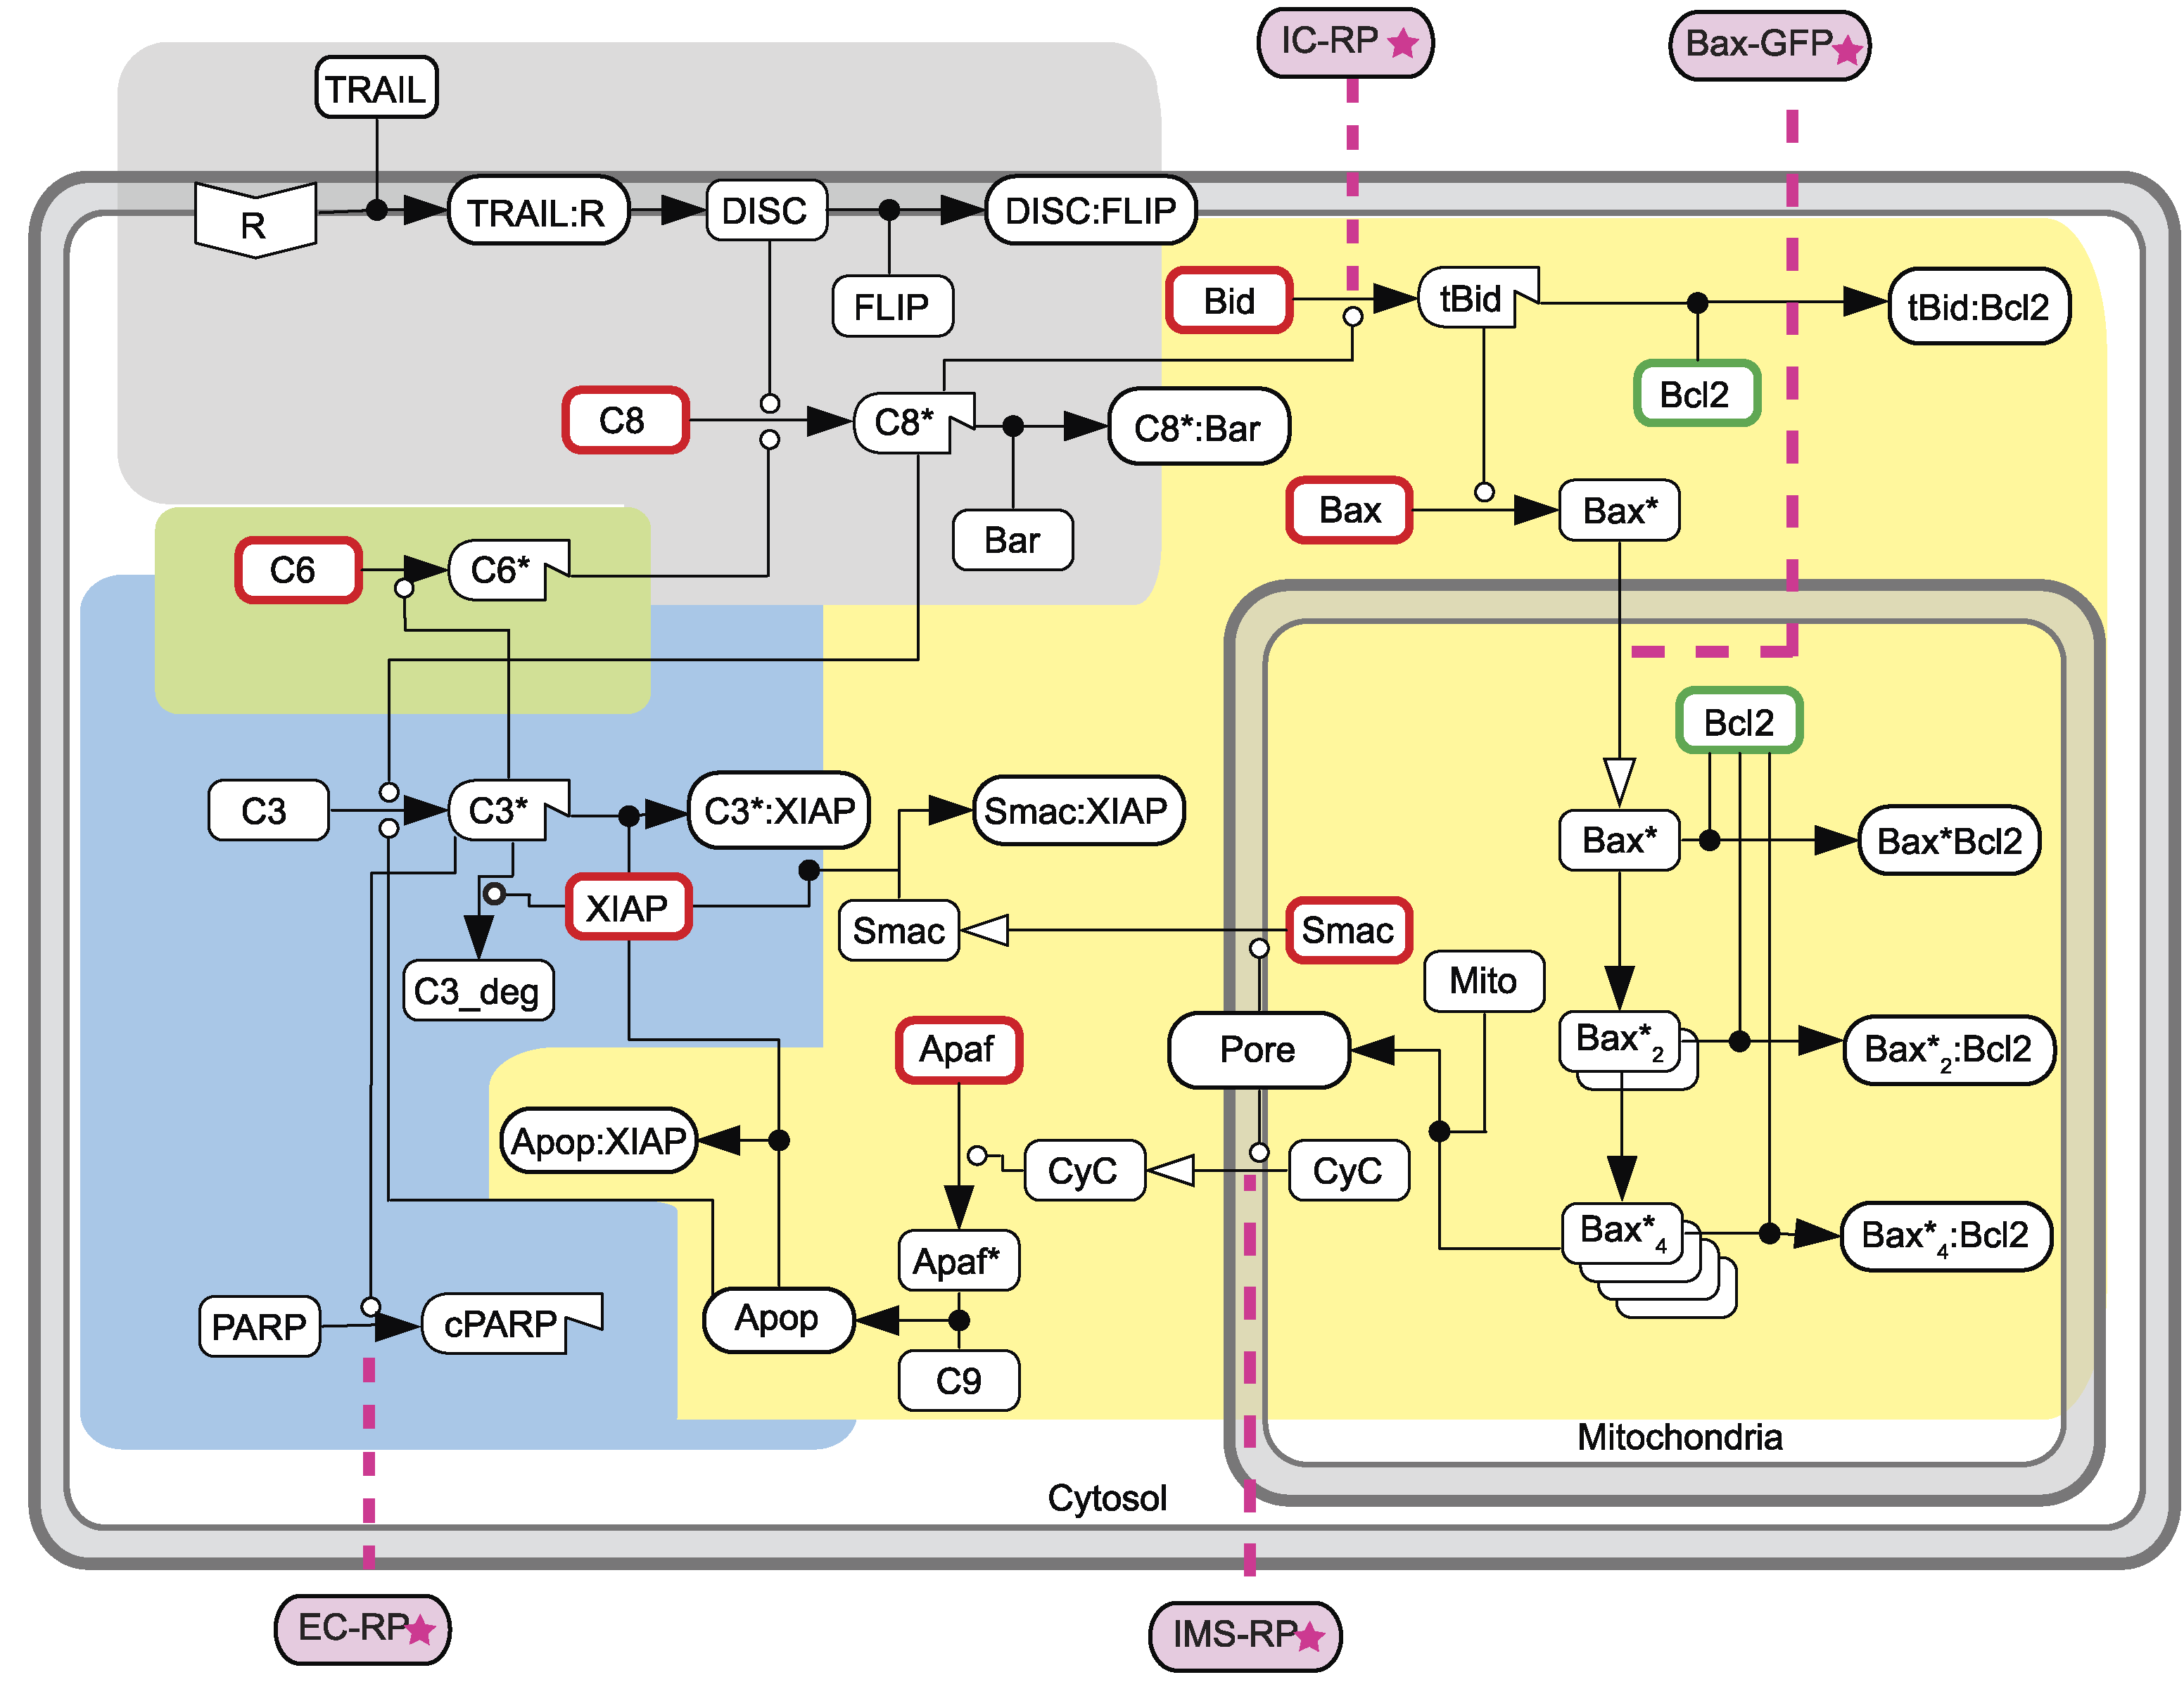
\includegraphics[width=0.9\textwidth]{./img/Cap3/ModeloCompleto.png}
    \caption{Esquema representativo de las reacciones modeladas por \textit{Sorger et al.} mediante ecuaciones diferenciales acopladas. Todas las especies que juegan un papel importante en la cascada de señalización caspasas se encuentran incluidas\cite{Albeck2008}.}
    \label{fig:ModeloCompleto}
\end{figure}

Como se muestra en la figura \ref{fig:ModeloCompleto}, el modelo puede dividirse en cuatro subcircuitos. El primero (gris) consiste en una representación agrupada de la unión del factor de necrosis tumoral (\ening{TNF} por sus siglas en inglés) o ligando de inducción de apoptosis relacionado con TNF (\ening{TRAIL} por sus siglas en inglés) al receptor y la subsecuente activación de la procaspasa-8 mediante el complejo de señalización de inducción de muerte (\ening{DISC} por sus siglas en inglés) unido al receptor. En segundo lugar (azul), se muestra la cascada enzimática en que la caspasa-8 activa cliva a la procaspasa-3, la cual a su vez cliva otros sustratos efectores. Por otro lado, se muestra la vía mitocondrial (amarillo) por la cual la caspasa-8 activa cliva a Bid para dar lugar a la activación de Bax que luego dara lugar a la formación de poros en la membrana mitocondrial por los cuales citocromo C (\ening{CyC} por sus siglas en inglés) y Smac son traslocados al citosol; una vez ahí, se forma el apoptosoma a partir de Apaf-1 y procaspasa-9, para clivar y activar aún más moléculas de caspasa-3. Por último, se representa (verde) un lazo de retroalimentación positivo entre la caspasa-3 y la procaspasa-8 mediado por la caspasa-6, que es clivada y activada por la caspasa-3\cite{Sorger2008}.

Sumado a las aproximaciones implícitas en ley de acción de masas, la construcción de este modelo agrega otras tres aproximaciones que deben tenerse en cuenta. En primer lugar, la formación de DISC y el apoptosoma que incluyen unión de varias proteínas fue simplificado usando una representación con parámetros agrupados. En segundo lugar, se omitió la síntesis de cualquier proteína. Por último, especies con actividades similares fueron representadas por una única especie, entre ellas están: caspasa-8 y caspasa-10, caspasa-3 y caspasa-7 y la familia de proteínas similares a Bcl-2\cite{Sorger2008}.

El modelo matemático diseñado por \textit{Sorger et al.} fue entrenado con datos experimentales que provienen de experimentos de microscopía de células vivas, citometría de flujo e inmunoblotting de células perturbadas con depleción de proteínas o sobreexpresión. El modelo fue entrenado para describir adecuadamente el comportamiento de células normales y perturbadas ante estímulos con TRAIL\cite{Sorger2008}.

El modelo desarrollado por \textit{Sorger et al.} se encuentra libre para descargar e implementar en \textit{MatLab}. Se descargó dicho modelo y se adaptó para que describa el comportamiento de las especies correspondientes al sensor utilizado. Para ello fue necesario, en primer lugar, probar el algoritmo para reproducir algunas de las imágenes de la publicación y comprender los efectos que producen las variaciones de distintos parámetros.


%%%%%%%%%%%%%%%%%%%%%%%%%%%%%%%%%%%%%%%%%%%%%%%%%%%
\section{Adaptación del Modelo}

Considerando que se desea evaluar la actividad de las tres vías de caspasas descriptas en la Introducción se adicionaron al sistema modelado tres sensores que son clivados por las caspasas-3, -8 y -9, para estudiar las vías efectora, extrínseca e intrínseca, respectivamente. Se añadieron tres especies distintas para cada sensor, a saber, el sensor sin clivar en estado dimérico, el sensor formando complejo con la caspasa y el sensor clivado en estado monomérico. Las constantes de unión, disociación y formación de producto se eligieron iguales a las correspondientes a las distintas caspasas ya que se asume que trabajan por igual sobre cualquiera de los distintos sustratos.

\begin{figure}
    \centering
    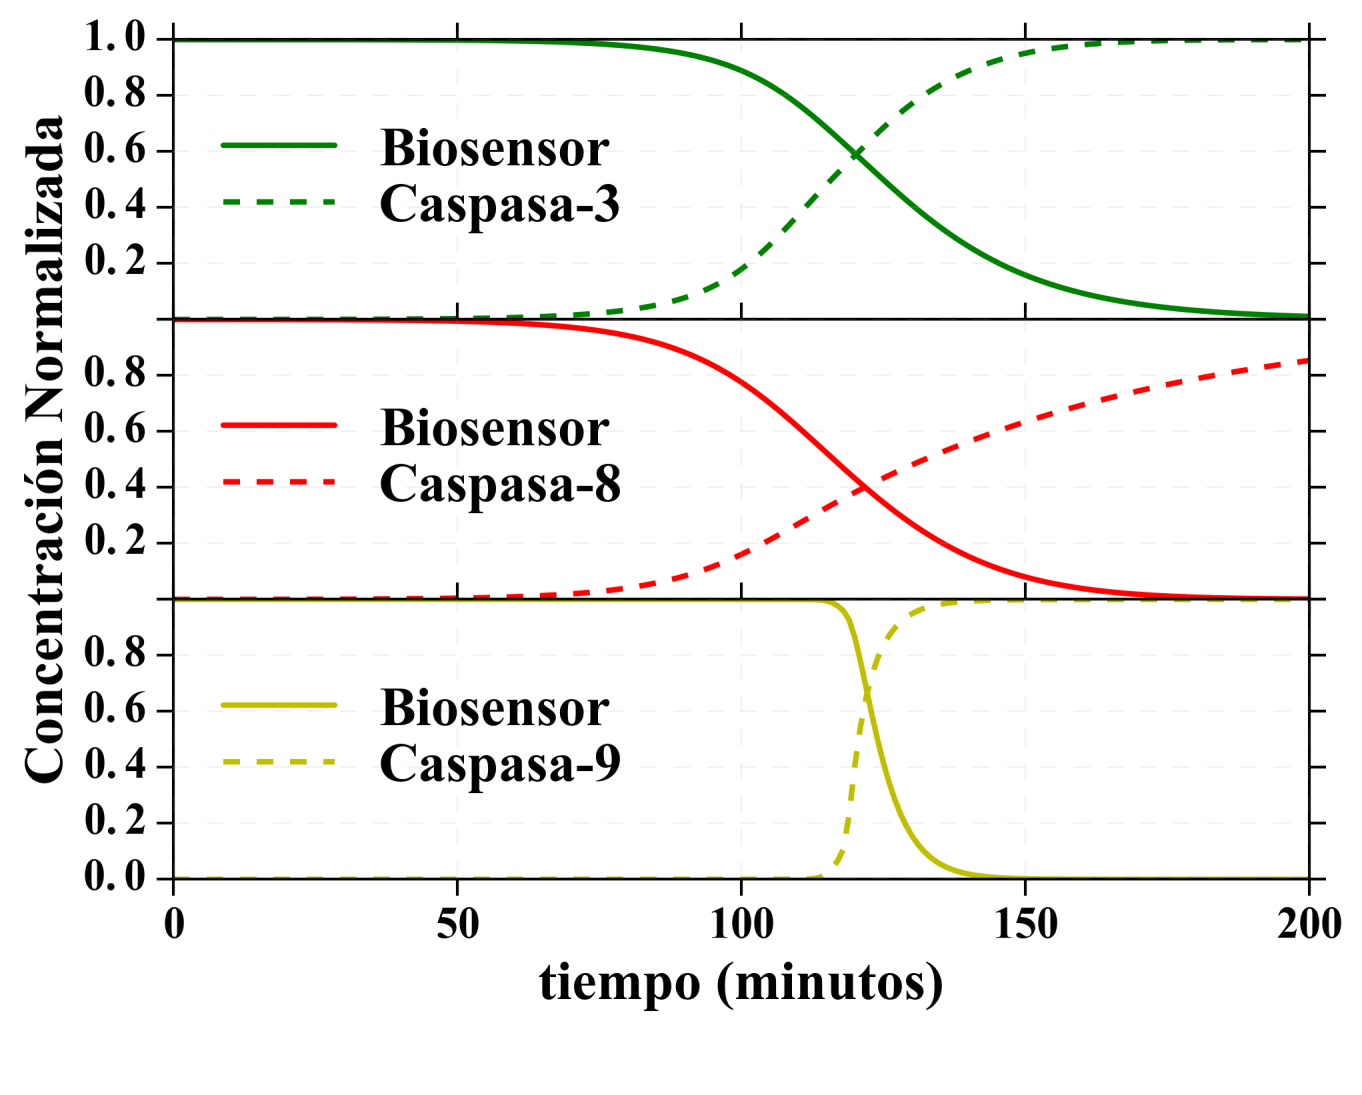
\includegraphics[width=0.65\textwidth]{./img/Cap3/AdicSensores.png}
    \caption{Se graficaron las concentraciones relativas de las tres caspasas de interés superpuestas con las correspondientes a los sensores adicionales del sistema biológico.}
    \label{fig:AdicSensores}
\end{figure}

Se asumió como hipótesis que los sensores sintetizados por la célula se producen en estado dimérico y estos son clivados únicamente por la caspasa activa de la célula durante la cascada de señalización. Por esta razón, se seleccionaron las condiciones iniciales de los sensores de forma tal que las concentraciones de las especies correspondientes al sensor clivado y en complejo sean nulas. Por otro lado, se debe tener una consideración especial al especificar la concentración inicial de sensor no clivado ya que concentraciones elevadas de esto producirán un fenómeno de secuestro sobre la caspasa evitando que esta cumpla su rol sobre el resto de la cascada de señalización.

Simultáneamente, se analizaron otras características del modelo matemático que fueron consideradas innecesarias para obtener una buena descripción del sistema en estudio. En particular, se le dio especial atención al hecho de que la caspasa-3 es la única que es degradada en el modelo y al lazo de retroalimentación entre las caspasa-3 y -8, mediado por la caspasa-6, que es despreciado por los autores solo al momento de observar las concentraciones en función del tiempo de todas las especies de interés.


%%%%%%%%%%%%%%%%%%%
\subsection{Análisis de Condiciones Iniciales de los Sensores}

Conocer los efectos del sensor sobre el sistema en estudio es importante para determinar si los datos obtenidos son una imagen fiel del sistema, o si la perturbación introducida no permite obtener información valiosa de este. Este razonamiento es análogo a cuando se desea medir caída de tensión en un circuito, y se busca que la resistencia interna del instrumental sea suficientemente alta para no perturbarlo de forma apreciable. Con el fin de comprender los efectos del sensor sobre el sistema, se realizaron varias simulaciones con el modelo adaptado utilizando diversas combinaciones de concentraciones iniciales para los distintos sensores.

En primer lugar podemos estudiar que sucede con la concentración del sensor clivado en función del tiempo para distintas concentraciones iniciales. La imagen \ref{fig:sweepcc} presenta las concentraciones de los sensores en función del tiempo utilizando distintas concentraciones iniciales, pero iguales entre sí en cada simulación. Puede apreciarse como a mayor concentración inicial de los sensores, más se demora la célula en clivarlo. Esto resulta intuitivo ya que la cantidad de caspasa trabajando se mantiene constante, pero la cantidad de sustrato para clivar aumenta.

\begin{figure}
    \centering
    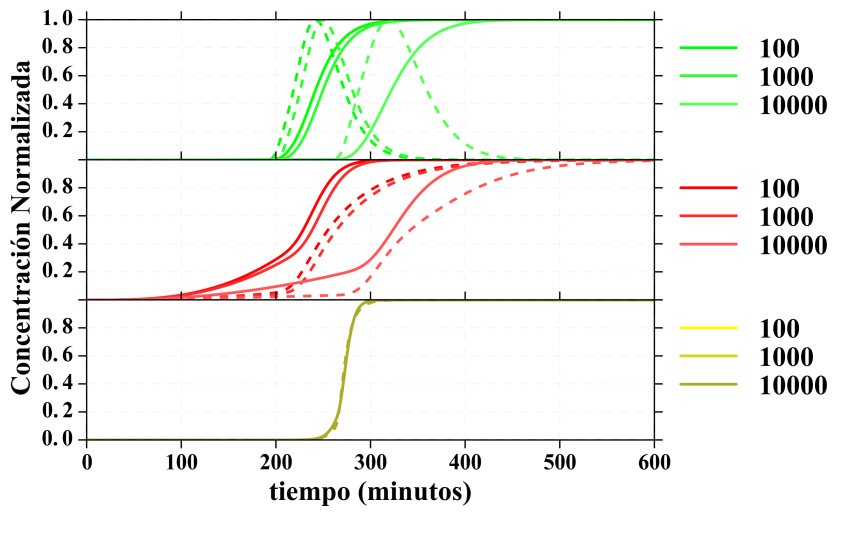
\includegraphics[width=0.9\textwidth]{./img/Cap3/SweepAll.png}
    \caption{Concentraciones normalizadas correspondientes a cada tipo de sensor sin clivar en función del tiempo para distintas concentraciones iniciales. Las concentraciones iniciales de cada sensor sin clivar se mantuvieron iguales entre sí en cada simulación.}
    \label{fig:sweepcc}
\end{figure}

%Por otro lado, es importante recalcar que cada sensor transfectado se hallaba en un plásmido distinto. Esto implica que no necesariamente se transfectaban los tres sensores simultáneamente a la misma célula, e incluso puede que más de una copia de alguno se haya transfectado a ésta.
Las concentraciones iniciales de cada sensor no son necesariamente iguales, pudiendo producir estancamientos en alguno de los pasos de la cascada de señalización. Los efectos de tener elevadas concentraciones iniciales de algún sensor puede implicar mayores diferencias temporales entre la activación de algunas caspasas y se explica mediante fenómenos de secuestro de enzima (caspasa) por el sustrato (sensor). Estos fenómenos de diferencias en concentraciones iniciales se traducen en retrasos temporales entre los tiempos en que se cliva cierto porcentaje del sensor. Consideremos, por ejemplo, lo que sucede con los momentos en que se cliva el 10$\%$ o el 50$\%$ del sensor. 

\begin{figure}
    \centering
    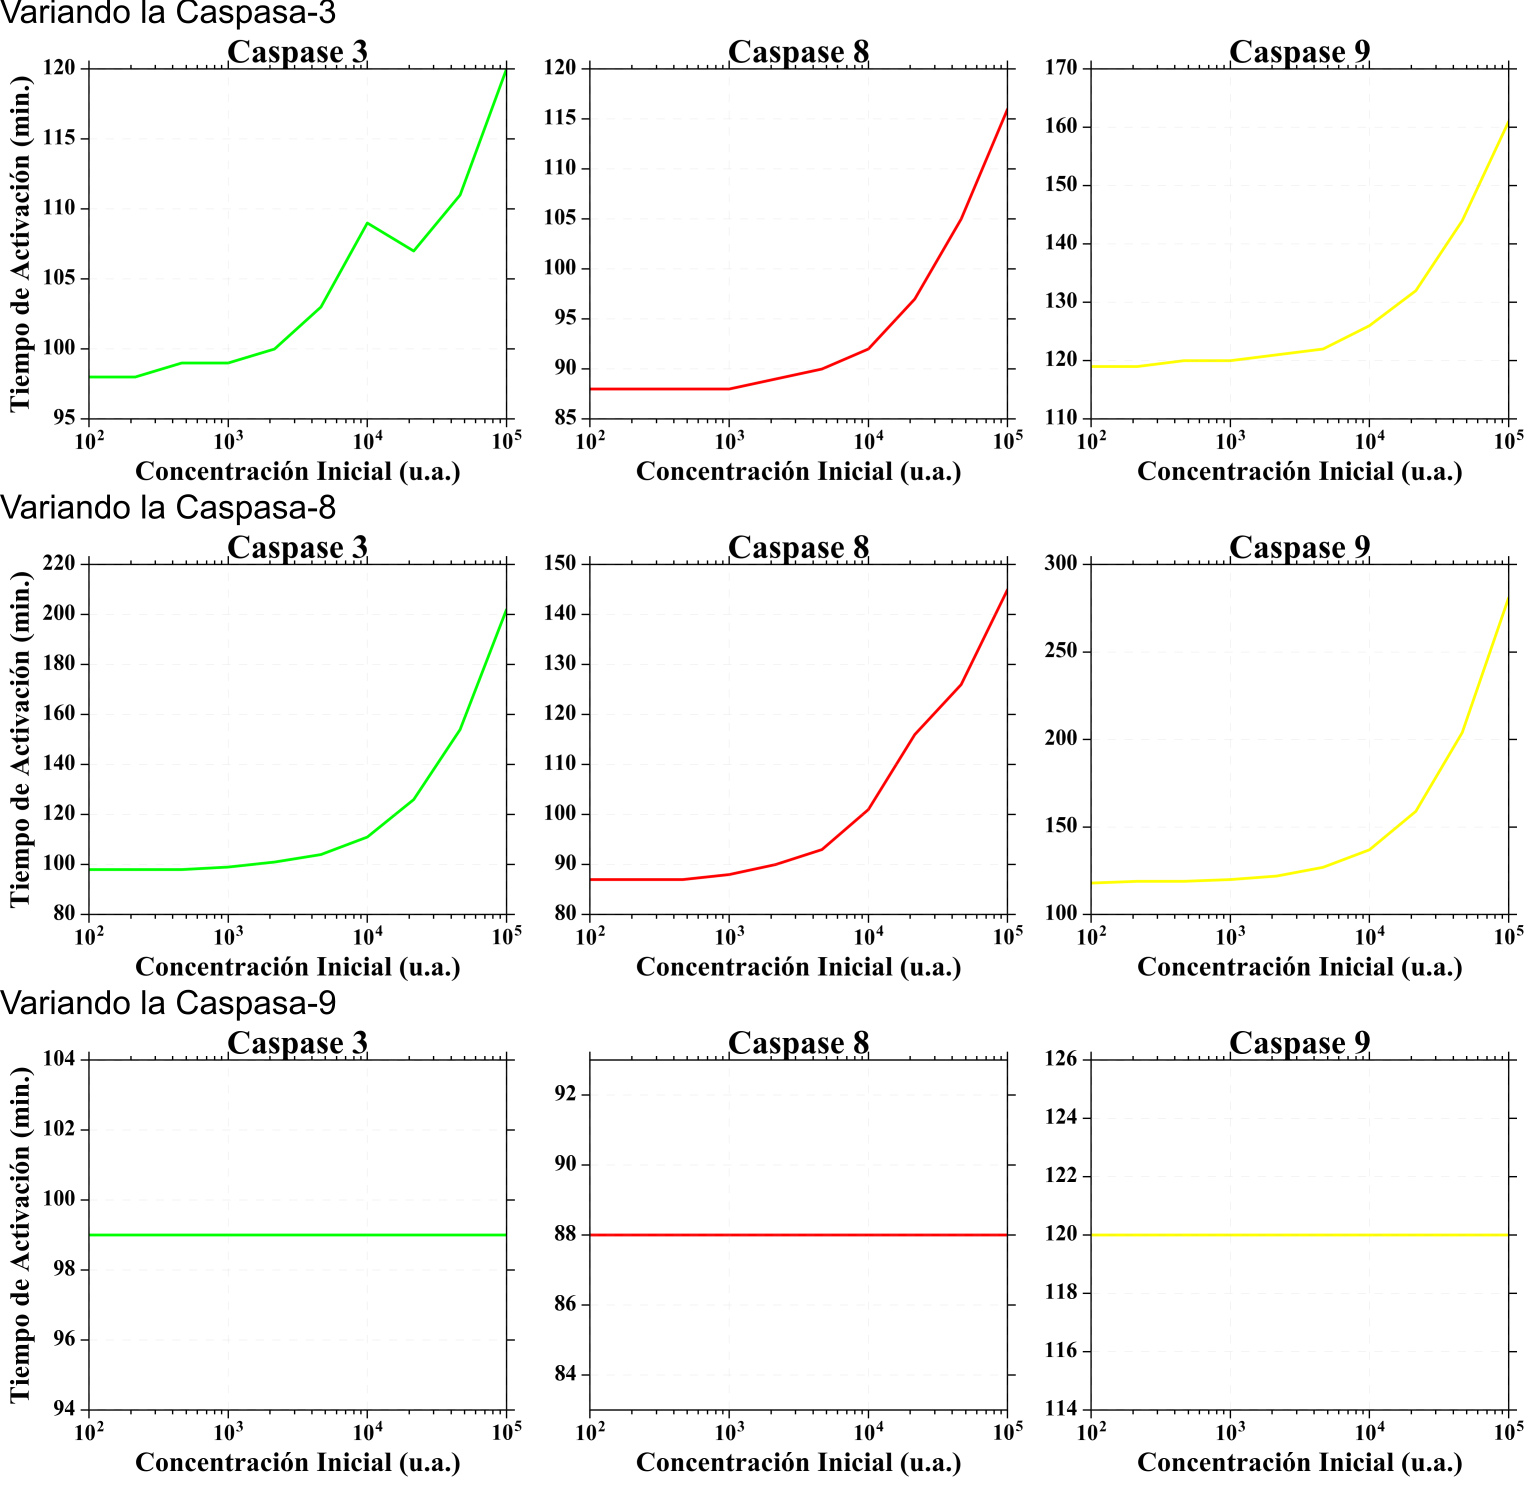
\includegraphics[width=0.9\textwidth]{./img/Cap3/Varcp10.png}
    \caption{Variación del momento en que se alcanza el clivaje de 10$\%$ de los biosensores utilizados. Se presentan en las distintas filas las simulaciones en que se variaba la concentración inicial de un único biosensor.}
    \label{fig:varcp10}
\end{figure}

En las figuras \ref{fig:varcp10} y \ref{fig:varcp50} se presentan gráficos del tiempo de activación definido como el momento en que se cliva el 10$\%$ o el 50$\%$ de sensor, respectivamente, según la concentración inicial de sensor utilizada. Este tipo de análisis provee información valiosa sobre el sistema y como se interrelacionan sus elementos. Tomemos por ejemplo la segunda fila de imágenes de la figura \ref{fig:varcp10} que corresponde a estudiar el momento en que se cliva 10$\%$ del sensor y se varia la concentración inicial del biosensor para caspasa-8. Se observa que la variación en el tiempo de activación de las tres caspasas. Esto se debe a que la caspasa-8, iniciadora en la vía extrínseca se encuentra menos alocada a activar la caspasa-3 y la vía intrínseca ya que se ve secuestrada por el biosensor. Aunque este tipo de análisis exhaustivo puede aplicarse a muchas simulaciones distintas, solo se presentarán las más relevantes para el trabajo realizado. Se debe destacar que la velocidad de la caspasa-9 es al menos un orden mayor que las otras, por esta razón no se ve afectada por fenómenos de secuestro.

\begin{figure}
    \centering
    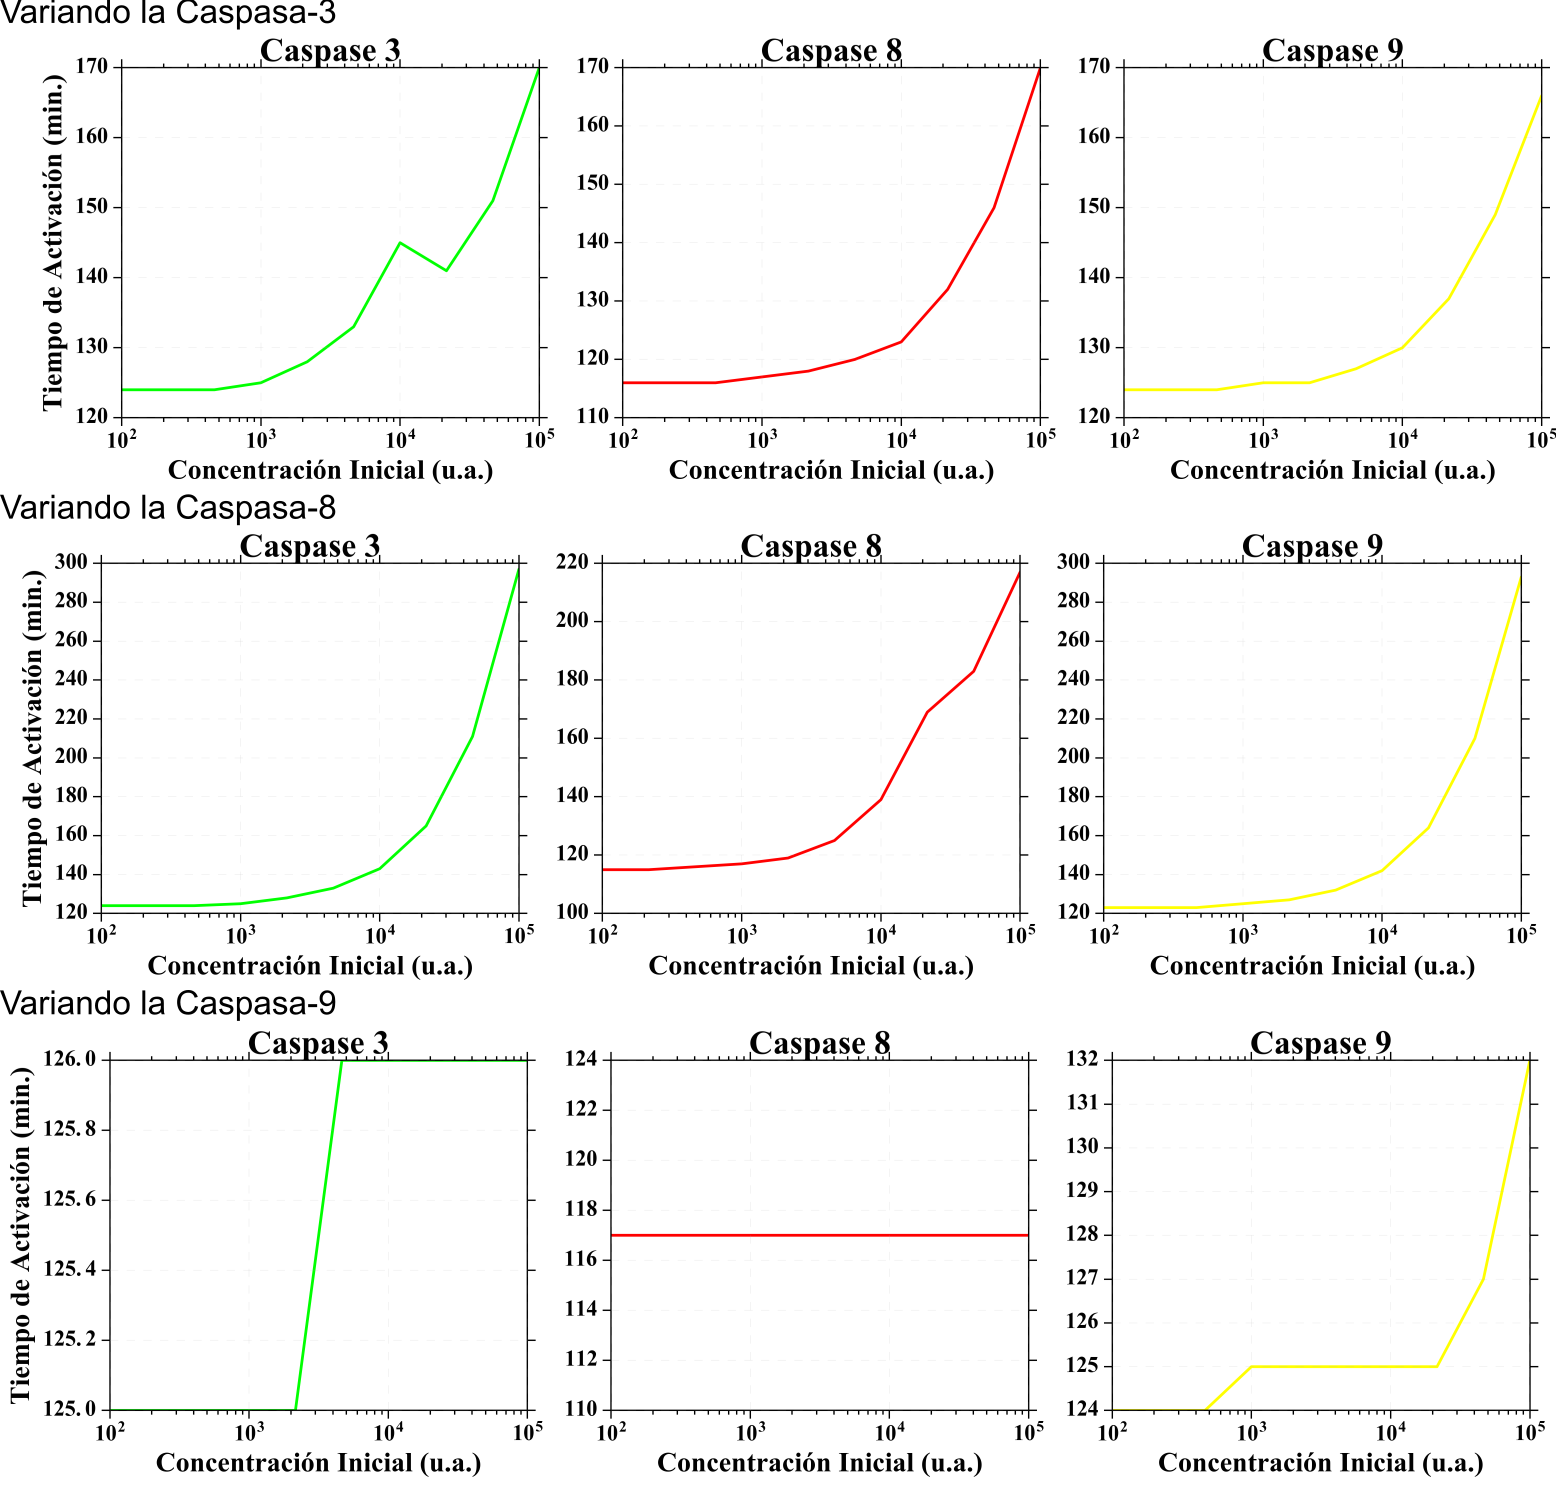
\includegraphics[width=0.9\textwidth]{./img/Cap3/Varcp50.png}
    \caption{Variación del momento en que se alcanza el clivaje de 50$\%$ de los biosensores utilizados. Se presentan en las distintas filas las simulaciones en que se variaba la concentración inicial de un único biosensor.}
    \label{fig:varcp50}
\end{figure}

Es importante destacar que las diferentes concentraciones de biosensor tienen doble efecto sobre el análisis que queremos realizar en el sistema. En primer lugar, cantidades elevadas de biosensor alteran la dinámica de la red produciendo resultados poco fieles a la dinámica fisiológica de este. Por otro lado, concentraciones bajas de biosensor implica que el clivaje total del sensor ocurrirá rápidamente y no será posible apreciar la dinámica de éste a tiempos largos.

%%%%%%%%%%%%%%%%%%%
\subsection{Degradación de la Caspasa-3}

A continuación, se estudiaron los efectos de incluir la degradación de la caspasa-3 en el modelo matemático. En primer lugar, se observó que si la caspasa-3 comienza a ser degradada inmediatamente después de ser activada, esta ejerce su función de clivaje durante una ventana temporal acotada. Esto se refleja, en parte, en que no todo el sensor disponible es clivado por la caspasa-3, como puede observarse en la imagen \ref{fig:deg_casp3}. Puede apreciarse que la proporción de caspasa activa comienza y termina en cero.

\begin{figure}
    \centering
    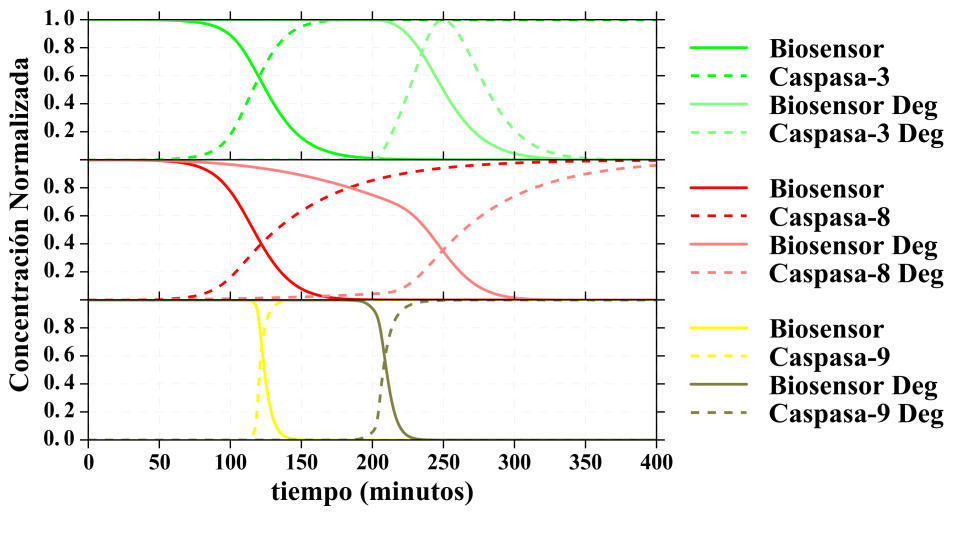
\includegraphics[width=0.9\textwidth]{./img/Cap3/ConSinDeg.png}
    \caption{Se presentan gráficos superpuestos de las curvas correspondientes al sensor sin clivar y la caspasa activa para las simulaciones en que se activaba la degradación de la caspasa-3 (Deg) y las que no.}
    \label{fig:deg_casp3}
\end{figure}

Por otro lado, se deben recalcar los efectos que la degradación o ausencia de degradación de la caspasa-3 tiene sobre el orden de activación de las caspasas. Resulta intuitivo que activar la degradación producirá no solo un retraso en su activación, sino que también se verá disminuida la actividad del lazo de retroalimentación con la caspasa-8, demorando a su vez la activación de esta otra caspasa. Estos efectos pueden deducirse de la cascada de señalización de caspasas.


%%%%%%%%%%%%%%%%%%%
\subsection{Lazo de Retroalimentación de la Caspasa-6}

Como se aprecia en la figura \ref{fig:ModeloCompleto}, el rol de la caspasa-6 es el de servir de medio de retroalimentación positiva entre la caspasa-3 activa y la procaspasa-8. En el trabajo presentado por \textit{Sorger et al.}, este mecanismo de retroalimentación es desactivado con el único fin de confeccionar una imagen. De todas formas, se decidió estudiar sus efectos en el modelo adaptado.

\begin{figure}
    \centering
    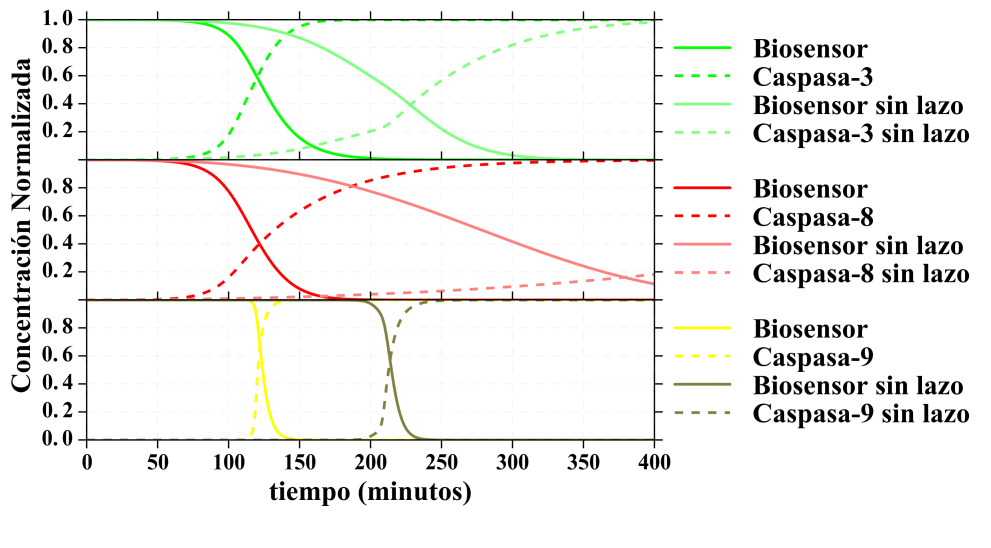
\includegraphics[width=0.9\textwidth]{./img/Cap3/ConSinC6.png}
    \caption{Se presentan gráficos superpuestos de las curvas correspondientes al sensor sin clivar y la caspasa activa para las simulaciones en que se activaba el lazo de retroalimentación de la caspasa-6 y los que no (sin lazo).}
    \label{fig:casp6}
\end{figure}

En la figura \ref{fig:casp6} se muestran los efectos que tiene el lazo de retroalimentación en estudio. Como es de esperarse, su papel principal es el de fomentar la activación de caspasa-8 una vez que se encuentra activa la caspasa-3. Su inactivación se ve reflejada en el incremento de la diferencia temporal que hay entre las activaciones de la caspasa-3 y -8.


%%%%%%%%%%%%%%%%%%%%%%%%%%%%%%%%%%%%%%%%%%%%%%%%%%%
\section{Estado de la Caspasa Inferido a Partir del Estado del Sensor}

Una vez adaptado el modelo matemático para incluir el comportamiento de los sensores, se analizaron que parámetros son útiles para recuperar información valiosa sobre el estado de este.
%Haciendo uso del método de ajuste presentado en el capítulo \ref{cap:microscopia}, que nos permite encontrar la proporción de fluoróforo en estado monomérico a partir de la curva de anisotropía del sistema, podemos implementar métodos para inferir el estado de la caspasa en estudio.

Conociendo la proporción de sensor en un estado clivado podemos estimar la cantidad de complejo caspasa:sensor calculando su derivada y normalizando. Esto se deduce utilizando la ecuación análoga a la ecuación \ref{eq:cin_prod} que relaciona la velocidad de formación de producto, o sensor clivado en este caso, con la concentración de complejo. Una posible interpretación de esta variable, $\Delta m$ es que representa la cantidad de caspasa que se encuentra clivando sensor en cada instante, es decir, ofrece una lectura sobre la actividad caspasa. %Esta claro que depende de la existencia de sensor sin clivar para poder ofrecer alguna lectura.

De todas formas, debe tenerse cuidado con su interpretación ya que solo funciona si la concentración del sensor en la célula se encuentra dentro de un rango dinámico comparable a otras especies de la célula. En particular, si hay poco sensor dentro de la célula, se observará una actividad máxima muy temprana que dura unos pocos minutos. Mientras que si la concentración del sensor es demasiado alta, la red de caspasas se verá muy perturbada por el sensor y el sistema presentará un comportamiento alejado de la realidad.

Debido a las constantes de reacción involucradas en las reacciones de clivaje del sensor, el modelo predice que las concentraciones de complejo caspasa:sensor son al menos cuatro ordenes más chicas que las concentraciones de sensor. A esto debe sumarse que por conservación de la cantidad de biosensor, $s+c+p$ es un valor constante, y si despreciamos $c$, podemos obtener el valor de $s$ a partir de $-p$.

A continuación, teniendo en cuenta el efecto que tiene la cantidad de sensor inicial sobre el parámetro relacionado con la actividad de la caspasa, se decidió dividir la derivada temporal de la proporción de sensor clivado por la concentración de sensor sin clivar. Este parámetro, que llamaremos $\Delta m/d$ normalizado nos reporta de forma robusta la proporción de caspasa activa. Puede apreciarse en la figura \ref{fig:Deltams} la superposición entre las especies normalizadas de complejo caspasa:sensor y caspasa activa con sus reporteros $\Delta m$ y $\Delta m/d$, respectivamente.

\begin{figure}
    \centering
    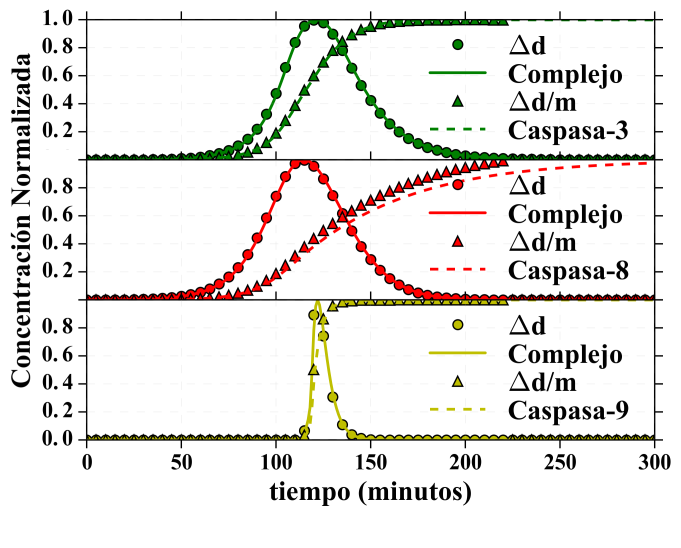
\includegraphics[width=0.9\textwidth]{./img/Cap3/Metodo.png}
    \caption{Gráfico de proporción de caspasa activa y caspasa en complejo con biosensor en función del tiempo y superpuesto con $\Delta m$ y $\Delta m/d$. Se puede apreciar la elevada similitud entre el complejo caspasa:sensor y $\Delta m$, así como también entre la caspasa activa y $\Delta m/d$.}
    \label{fig:Deltams}
\end{figure}

Existen diversas consideraciones que deben tenerse en cuenta para analizar este parámetro. Para comprender mejor de donde surge este parámetro, podemos apreciar que antes de que se active la caspasa, la cantidad de sensor sin clivar es máxima, mientras que como no hay variaciones en la proporción de sensor clivado el valor de $\Delta m/d$ nos reporta que la proporción de caspasa activa es nula. Si nos concentramos en el otro extremo, la cantidad de sensor sin clivar tiende a cero, al igual que la variación de sensor clivado. Si el numerador y denominador tienden a 0, pero el denominador lo hace más rápido, entonces al normalizar observaremos que la proporción de caspasa activa es máxima, y se corresponde con el estado del sistema.

Para comprender que sucede durante la transición será necesario considerar despreciable la concentración total de complejo caspasa:sensor frente a la concentración total de enzima y sensor libre. Dado que el modelo matemático se condice con esta aseveración, podemos utilizar la ecuación \ref{eq:cin_sens} para mostrar que despreciando el valor de $c$, llegamos a que

\begin{equation}
    \frac{ds}{dt} = - k_+ se,
\end{equation}

\noindent de donde se deduce que dividir la variación de sensor en estado dimérico por su concentración es proporcional a la cantidad de enzima activa. De esta forma, es válido utilizar $\Delta m/d$ (ó $\Delta p/s$) normalizado para estimar la proporción de caspasa activa. También deben tenerse los mismos recaudos que se tuvieron para $\Delta m$ si se utilizan concentraciones iniciales de sensor muy altas o muy bajas.

Finalmente, se repitieron los cálculos para distintas simulaciones donde se utilizaron diferentes concentraciones iniciales para cada sensor. Se recuperaron adecuadamente las curvas normalizadas de complejo caspasa:sensor así como la proporción de caspasa activa para todas las simulaciones, excepto cuando las concentraciones utilizadas eran exageradas. De esta forma, se deduce que dentro del rango de concentraciones posibles para el sensor, este estudio reporta adecuadamente la proporción de caspasa activa.


%%%%%%%%%  Información Biológica
\chapter{Información Biológica}
\label{cap:informacion}

Habiendo explicado los diferentes métodos de ajuste en el capítulo \ref{cap:microscopia} y aclarado como obtener la proporción de caspasa activa a partir del estado del ensamble de fluoróforos en el capítulo \ref{cap:modelo}, procedemos a presentar el experimento realizado del cual se obtuvieron los datos para analizar. Dicho experimento se realizó en el instituto Max Planck de alemania en el marco del proyecto \ening{Biocompatible multitasking nanoparticles for spatiotemporally resolved monitoring and photoinactivation of cancer cells and antibiotic resistant bacteria} financiado por el \ening{Deutsche Forschungsgemeinschaft} (DFG).

En este capítulo, los métodos desarrollados y explicados previamente serán aplicados al sistema en estudio para obtener información valiosa sobre el funcionamiento de este, además de brindar una mayor comprensión sobre los métodos utilizados. Por otro lado, se analizarán las posibles fuentes de error y falencias experimentales, así como posibles correcciones al protocolo experimental.


%%%%%%%%%%%%%%%%%%%%%
\section{Armado Experimental}

Si bien el experimento no se realizó en el laboratorio, este consistió fundamentalmente en preparar un cultivo celular que exprese los biosensores para las caspasas deseadas, para luego proceder a estimular la inicialización de apoptosis en estas células y observar la dinámica de los biosensores. El primer paso fue desarrollar mediante ingeniería genética el plásmido que sería transfectado a la célula. Éste consiste en una secuencia de ADN que contiene la información necesaria para que la célula en cuestión pueda sintetizar alguna proteína en particular. Durante la transfección, se condiciona a la célula para que pueda recibir material genético externo, por medio del plásmido, para luego poder procesarlo como propio.

Una vez que las células expresan los biosensores transfectados, estas deben ser inducidas para entrar en apoptosis mediante algún estímulo como staurosporina o TNF-$\alpha$, si se desea inicializar por la vía extrínseca, o especies reactivas del oxígeno, si se desea estimular la vía intrínseca. Habiendo inducido a la célula, solo resta adquirir imágenes de los observables fotofísicos para proceder a su análisis y estudio del sistema biológico.

\subsection{Diseño de Biosensores}

Tres biosensores basados en homoFRET fueron diseñados para luego ser transfectados a las células en estudio. Las combinaciones de fluoróforos utilizados fueron TagBFP con mCerulean, mCitrine con mCitrine y mCherry con mKate, cuyos espectros se muestran en la figura \ref{fig:EspectroFluos}. Los biosensores se construyeron insertando el segundo fluoróforo amplificado por PCR y delimitado por los sitios de restricción de Spe1 y Sal1 y conteniendo un codon STOP en los sitios de restricción Spe1/Sal1 de un vector-C1 (Clontech). Adicionalmente, el producto de PCR tenía una secuencia de unión en el extremo 5'. Estos plásmidos se utilizaron como controles no clivables. Por otro lado, para construir los sensores clivables por la caspasa, se utilizaron las secuencias que codificaban para los sitios de clivado de las caspasas-3, -8 y -9 (DEVD, IETD-IETD, LEHD, respectivamente) fueron amplificadas por PCR y delimitadas por sitios de restricción BSP1 y Spe1, y luego subclonados a los sitios de restricción correspondientes en los plásmidos de control no clivables, volviendolos plásmidos que codifican para el sensor clivable.

\begin{figure}
    \centering
    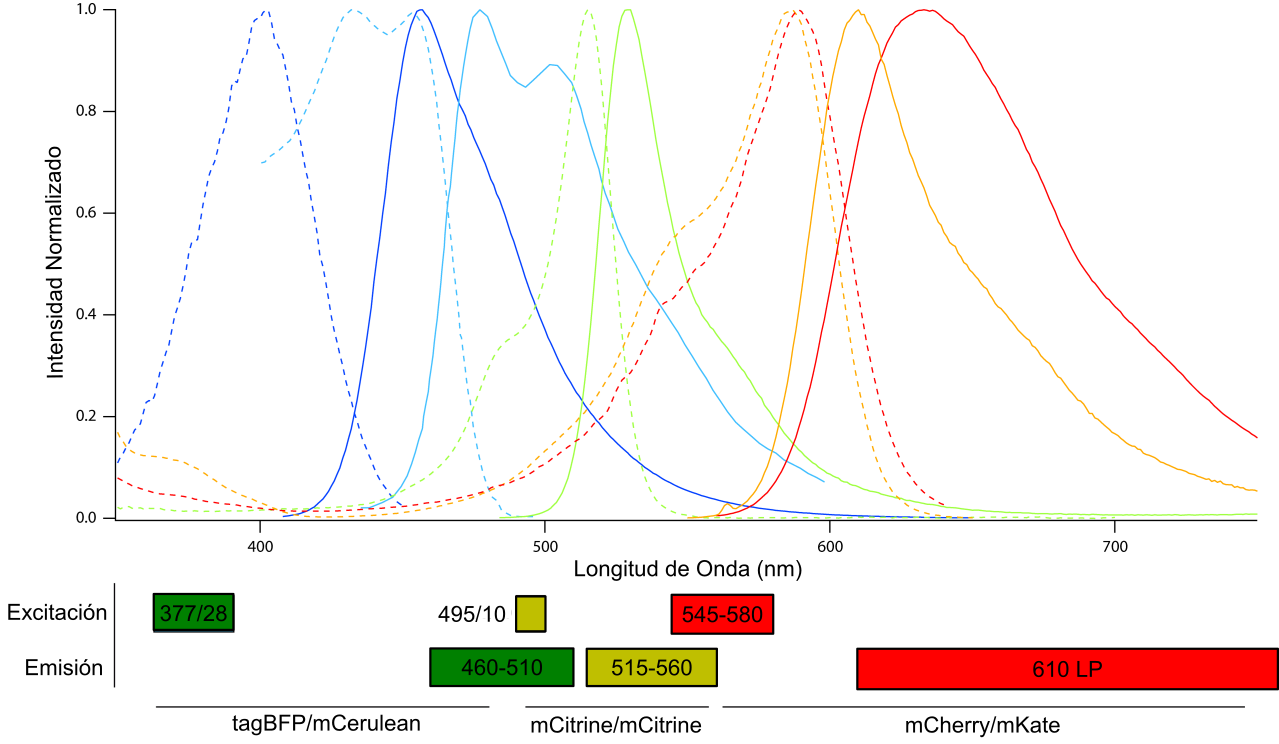
\includegraphics[width=0.9\textwidth]{./img/Cap4/spectra_w_filters.png}
    \caption{Espectro de excitación y emisión de los fluoróforos utilizados. Se muestra también los filtros utilizados en la adquisición.}
    \label{fig:EspectroFluos}
\end{figure}

\subsection{Cultivo Celular}

Se cultivaron células Hela en medio DMEM (PAN Biotech) suplementado con 10$\%$ suero fetal de cabra (FCS, Gibco), 100 U/ml de penicilina, 100$\mu$g/ml de streptomicina, 1$\%$ de L-glutamina y 1$\%$ de aminoácidos no esenciales (todos de PAN Biotech) a 37$^{\circ}$C y 5$\%$ de CO$_2$ en una incubadora humidificada. El día anterior a la transfección las células fueron traspasadas a discos de 8 \ening{wells} (LabTekII, Nalgene) a una densidad de $3\times10^4$ células. La transfección se concretizó utilizando Fugene 6 (Promega) siguiendo el protocolo del manufacturante. 20 horas después de la transfección, las células fueron observadas en DMEM sin rojo fenol (PAN Biotech) y 0$\%$ FCS en presencia de 1$\mu$M de staurosporina (Sigma Aldrich, Alemania) junto con 10$\mu$g/ml de ciclohexamida (Sigma Aldrich, Alemania) para inducir apoptosis e inhibir la síntesis proteíca.

\subsection{Adquisición de Imágenes}

Las imágenes fueron adquiridas mediante un setup customizado en Alemania. Se utilizó un microscopio invertido Olympus IX-81 equipado con un sistema de iluminación MT20. Se adicionaron tres polarizadores dicroicos Meadowlark Optics, Frederick, Colorado, US), uno en el camino óptico de excitación del microscopio y los otros dos fueron colocados con sus ejes perpendiculares entre sí en una rueda de filtros en el exterior del microscopio (ver figura \ref{fig:armadoExp}). La fluorescencia se colectó utilizando un objetivo de aire de 20$\times$ y apertura numérica de 0,7. Las imágenes en las polarizaciones paralela y perpendicular se adquirieron secuencialmente utilizando una cámara CCD Orca (Hamamatsu Photonics, Japan). El software CellR (Olympus, Alemania) fue utilizado para controlar la adquisición. Previo a cada experimento se tomaron imágenes de una muestra de referencia, siendo esta fluoresceína diluida. Estas se tomaron a 37$^{\circ}$C usando un sistema de control de temperatura que consistió en un calentador de objetivo y el calentador de especimen Stable Z (Bioptechs Inc., Butler, PA, USA). Estas últimas se utilizaron para calibrar el sistema calculando el factor G.

\begin{figure}
    \centering
    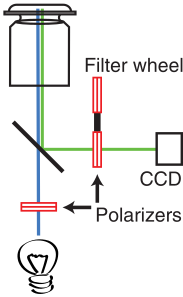
\includegraphics[width=0.2\textwidth]{./img/Cap4/ArmadoExp.png}
    \caption{Esquema del camino óptico del armado experimental donde se detalla la ubicación de los polarizadores utilizados.}
    \label{fig:armadoExp}
\end{figure}

\subsection{Procesamiento de Imágenes}

En primer lugar, se utilizaron las imágenes adquiridas de la solución diluida de fluoresceína para corregir inhomogeneidades en la iluminación. Para ello, se dividio pixel a pixel, las imágenes de ambas polarizaciones con su correspondiente imagen de fluoresceína.Dado que el valor de anisotropía de la fluoresceína es muy cercano a cero, este procedimiento también sirve para corregir con el factor G, como se explicó previamente, el factor G da cuenta de las diferencias en sensibilidad de cada dirección de polarización observada.

A continuación, se sustrajo el ruido de fondo de las imágenes usando como valor de ruido de fondo la intensidad promedio de una región afuera de las células. Luego, debido a que los polarizadores introducen un corrimiento entre las imágenes de ambas polarizaciones, y considerando que este es el mismo para todas las imágenes, se busco corregir este corrimiento.

Una vez corregidas las imágenes adquiridas, se procedió a generar máscaras mediante un software de análisis de imágenes llamado \ening{Cell Profiler}. Este permitió identificar a las células como objetos, además de delimitar sus bordes. Para ello, el software selecciona un umbral de intensidad a partir del cual considera como parte del objeto todos los pixeles que sean más brillantes que el umbral, además de considerar regiones separadas como objetos distintos. Luego, se calculó el promedio de las intensidades paralela y perpendicular de cada célula, para calcular después la anisotropía utilizando la ecuación \ref{eq:anisotropia}. Un esquema de este procedimiento se presenta en la imágen \ref{fig:esqexp}.

\begin{figure}
    \centering
    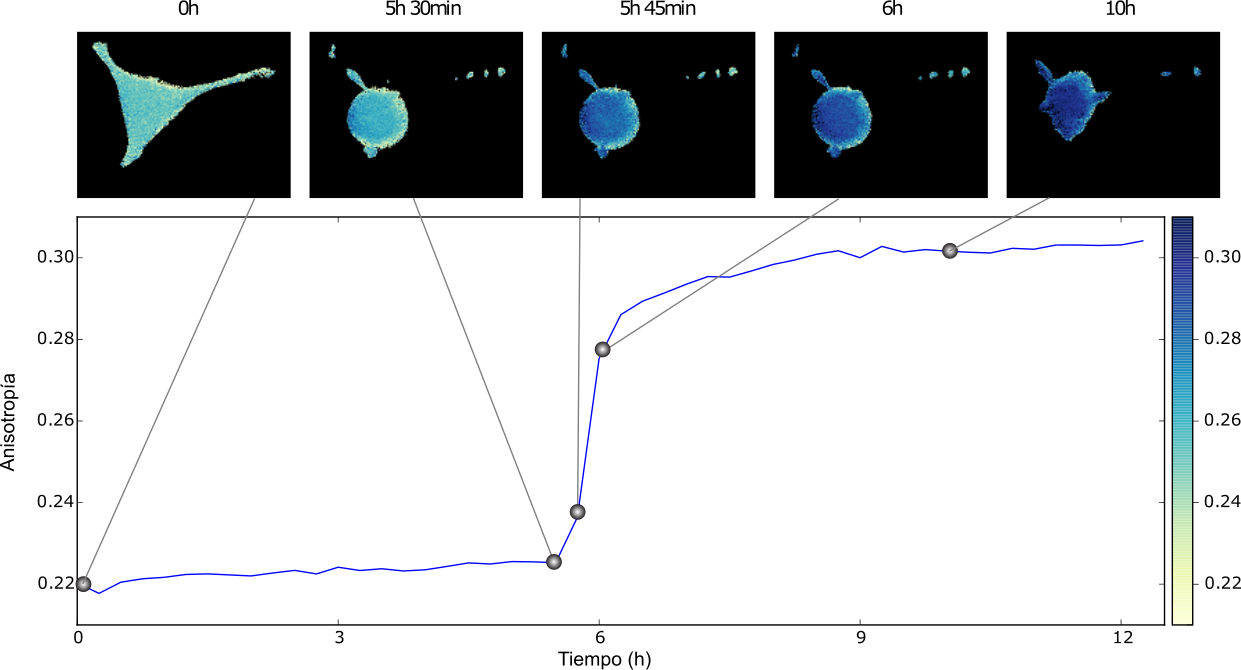
\includegraphics[width=0.9\textwidth]{./img/Cap4/EsqExp.png}
    \caption{En la sección superior se presenta una serie temporal de las imágenes adquiridas de una célula en particular durante el proceso de apoptosis. Se presenta en escala de azules la anisotropía observada en cada pixel. Puede apreciarse como cambia la máscara de la célula a medida que disminuye la intensidad de algunos pixeles. Simultáneamente, podemos apreciar la curva de anisotropía calculada para esta célula.}
    \label{fig:esqexp}
\end{figure}


%%%%%%%%%%%%%%%%%%
\section{Curvas}

Con el objetivo de obtener las curvas de anisotropía e intensidades total, paralela y perpendicular, que serían utilizadas para evaluar el sistema se realizaron los siguientes procedimientos. En primer lugar, luego de recibir los datos, se ajustaron todas las curvas de anisotropía por una función sigmoidea, es decir,

\begin{equation}
    f(x) = base + \frac{amplitud}{1+e^{k(x-x_0)}},
\end{equation}

\noindent donde la base y amplitud se refieren a los valores estables que adquiere la función para x mucho menores o mayores que $x_0$, respectivamente. El parámetro $k$ esta asociado con la velocidad de transición de un valor estable al otro, mientras que $x_0$ determina el valor de $x$ para el que la función se halla en el punto medio entre ambos valores. Esta función es la misma que se utilizó en el capítulo \ref{cap:microscopia} para generar la curva simulada de proporción de fluoróforo en estado monomérico.

Dado que la adquisición y el procesamiento de imágenes fue automatizado, muchas de las curvas obtenidas correspondían a artefactos de medición. Con el objetivo de filtrar los más de 3000 objetos identificados, se utilizaron los parámetros de la función sigmoidea para filtrar las curvas correspondientes a células en apoptosis de las que no. De esta forma, se identificaron 121 células con sus 3 curvas correspondientes a los tres biosensores que podían ser analizadas. En la figura \ref{fig:Aniso_ej} se presenta un ejemplo de las tres curvas de anisotropía de cada sensor correspondientes a una misma célula. Por otro lado, en la figura \ref{fig:todas} se muestra una superposición de todas las curvas de anisotropía filtradas y centradas para apreciar su forma funcional.

\begin{figure}
    \centering
    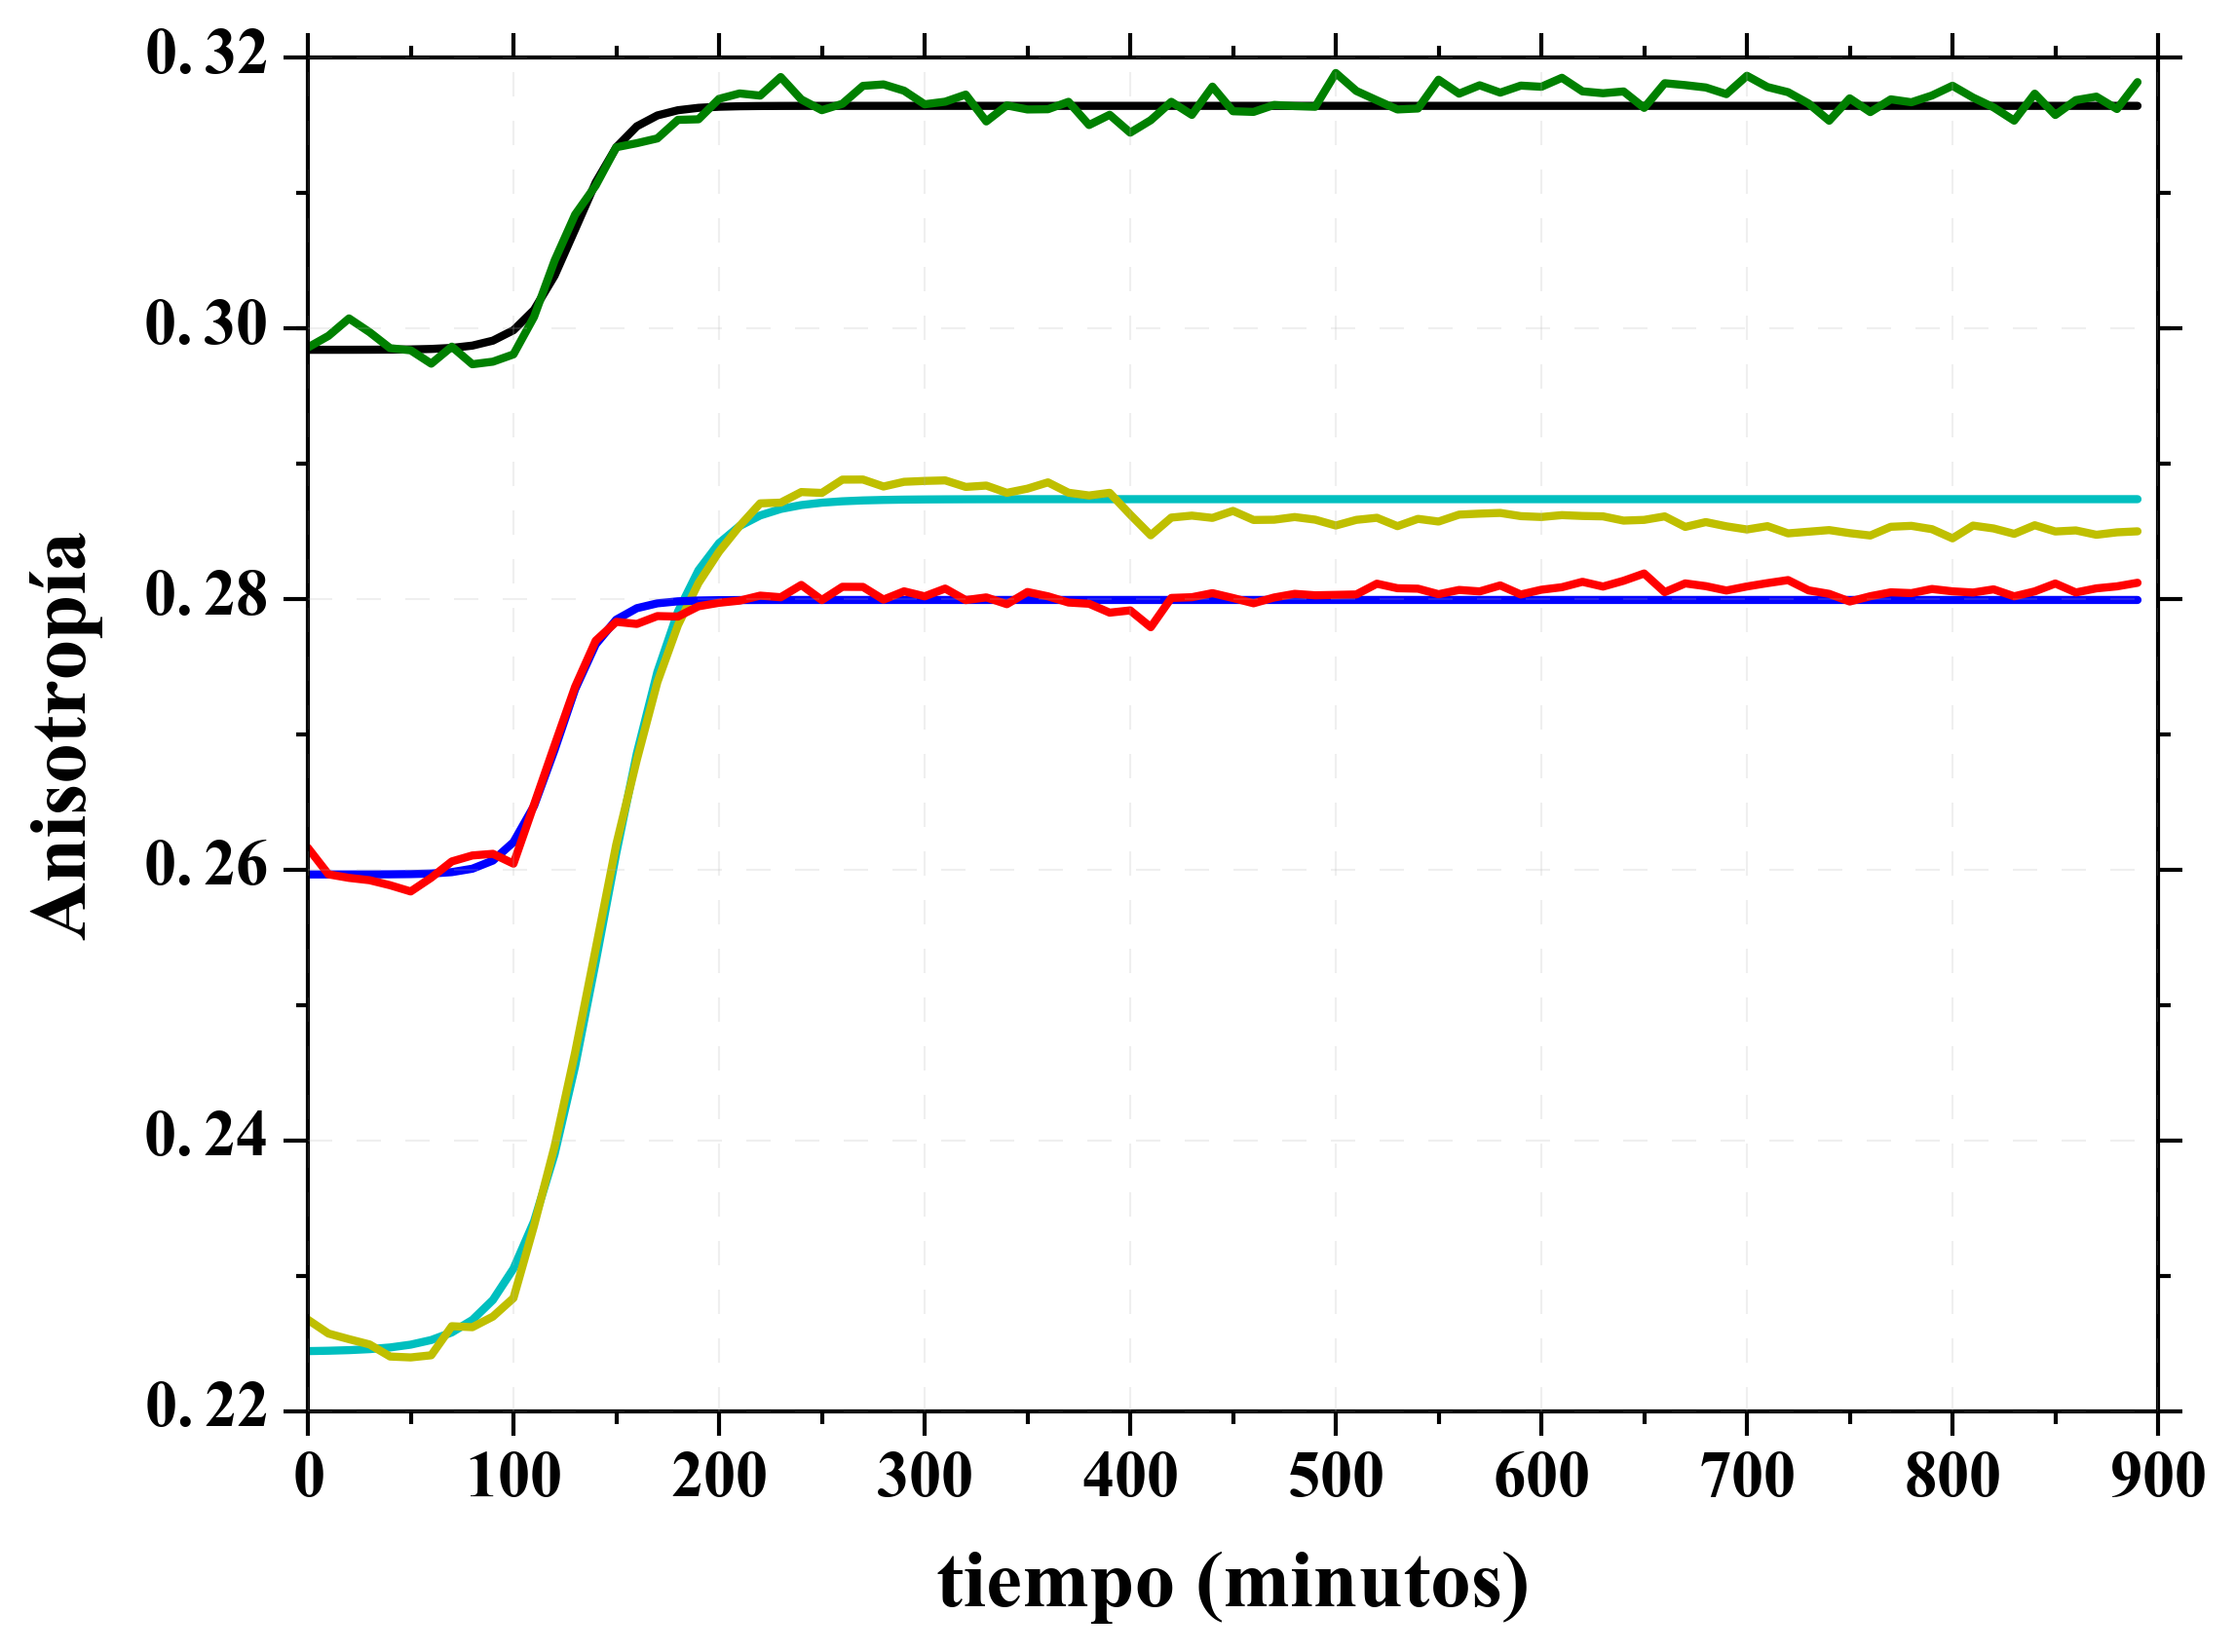
\includegraphics[width=0.6\textwidth]{./img/Cap4/Anisotropia2145.png}
    \caption{Gráfico de anisotropía en función del tiempo de cada sensor correspondientes a una misma célula.}
    \label{fig:Aniso_ej}
\end{figure}

\begin{figure}
    \centering
    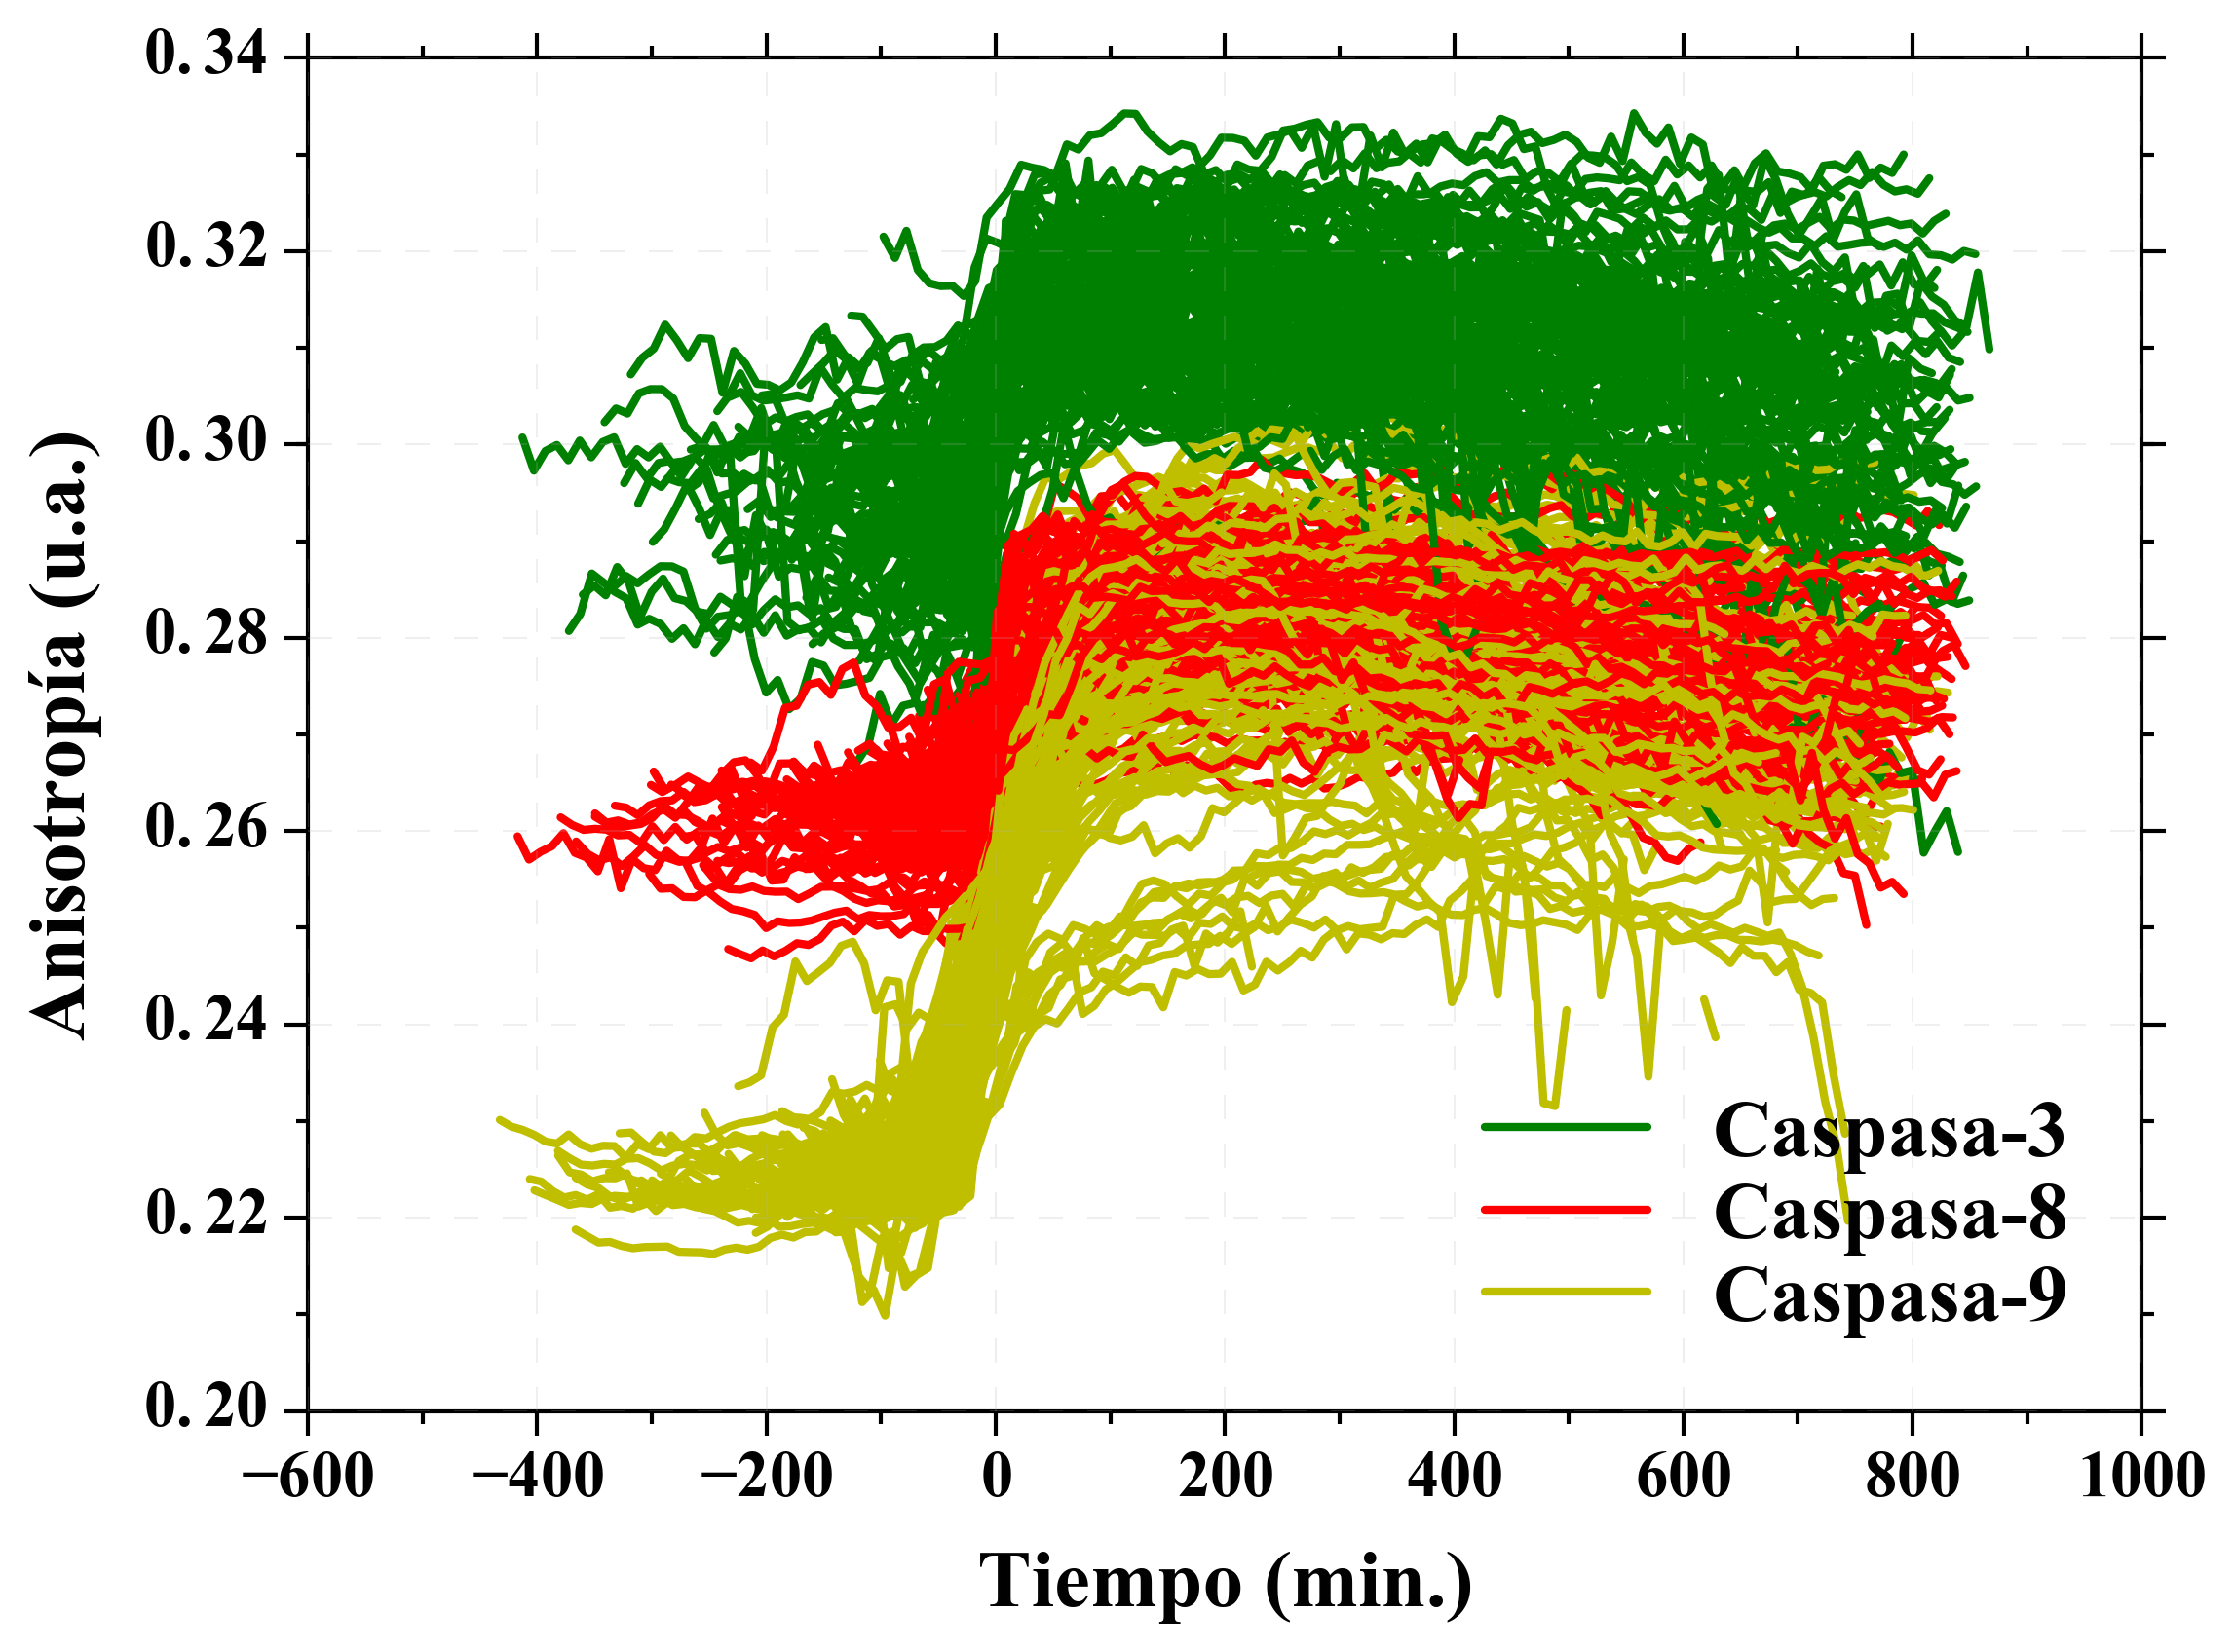
\includegraphics[width=0.6\textwidth]{./img/Cap4/AnisoJuntas.png}
    \caption{Gráfico de anisotropía en función del tiempo de todos los biosensores en todas las células. Se aplicó un corrimiento a todas las curvas para centrarlas y apreciar la forma de estas.}
    \label{fig:todas}
\end{figure}

Considerando que durante la adquisición de imágenes el foco no podía ser controlado automáticamente y teniendo en cuenta que la degradación de proteínas pueden llegar a tener un efecto sobre la anisotropía, se confeccionaron funciones que, basadas en los parámetros obtenidos de los ajustes previos, toman para analizar únicamente la región de la transición. Estas funciones se utilizaron para recortar las regiones de interés en las curvas de anisotropía.

Una vez halladas las curvas que se estudiarán resulta valioso comenzar con un análisis estadístico de los parámetros más importantes disponibles. Entre ellos, podemos estudiar las anisotropías del monómero y dímero, al igual que su diferencia o rango dinámico. Utilizando como hipótesis que el experimento se inicia con la totalidad del biosensor sin clivar y culmina con la totalidad del sensor clivado, se tomaron los diez valores de anisotropía que delimitaban las curvas recortadas para estimar los valores de anisotropía del dímero y del monómero.

\begin{figure}
    \centering
    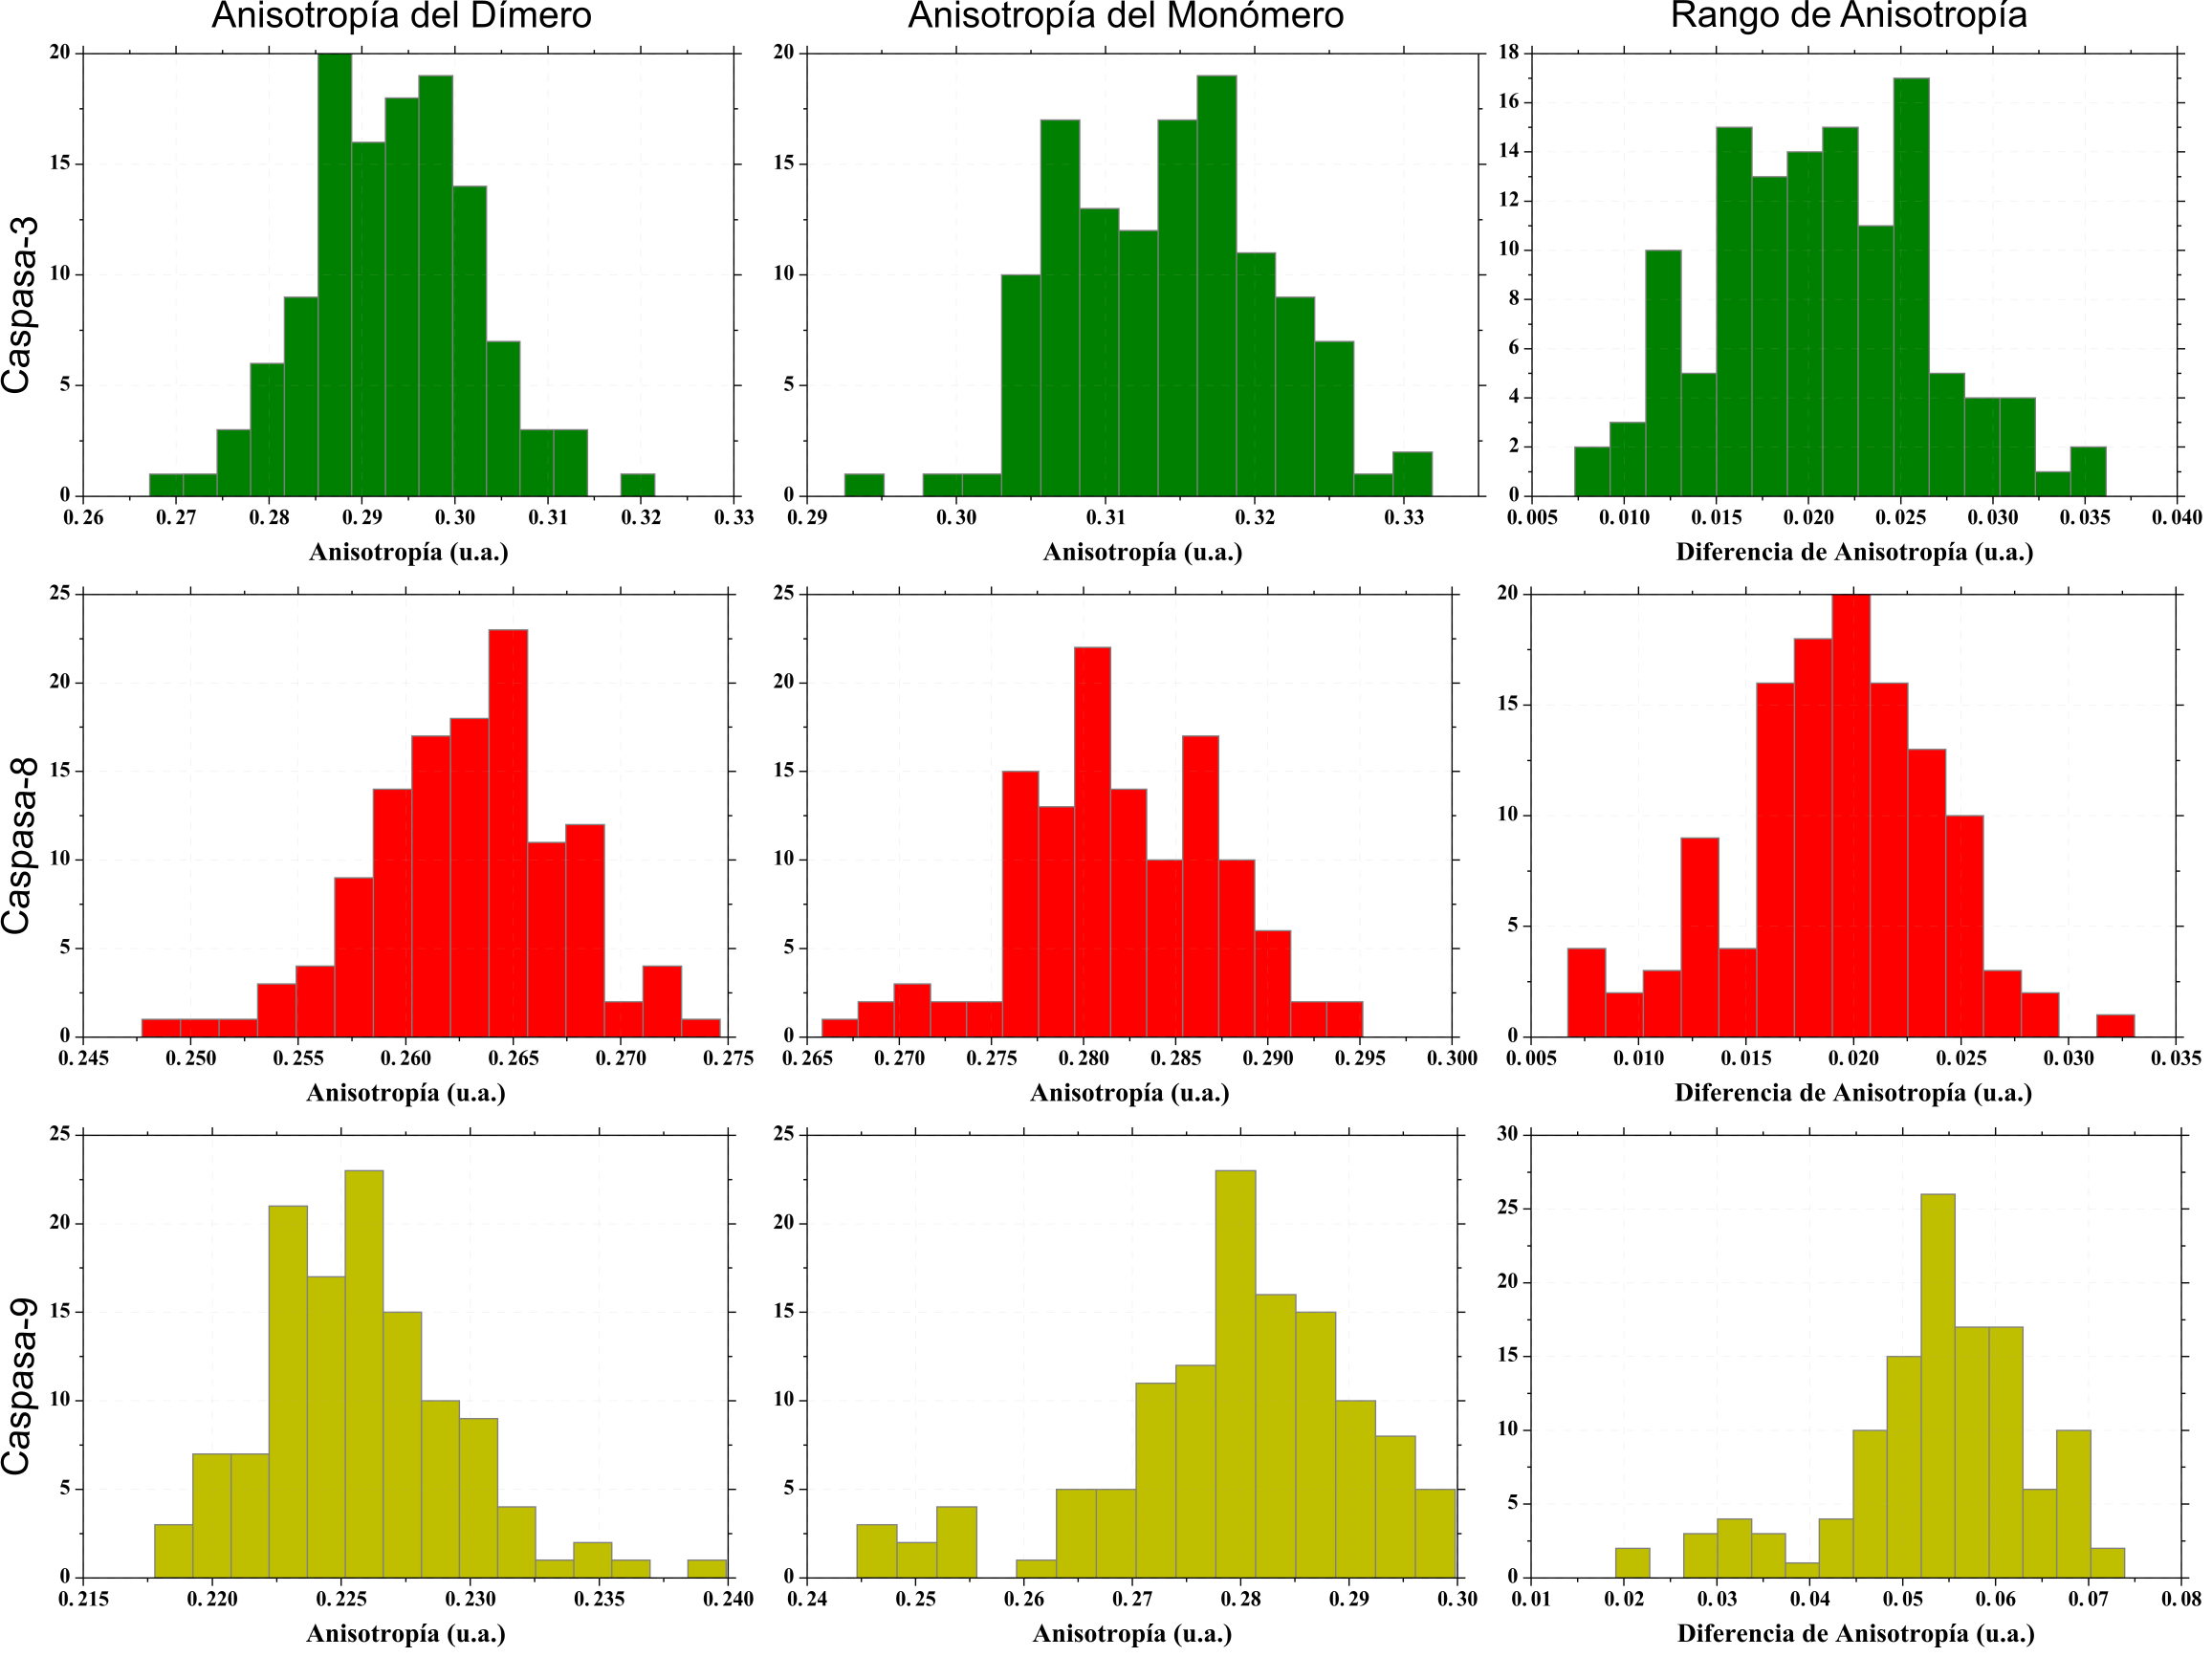
\includegraphics[width=0.9\textwidth]{./img/Cap4/HistogramasAnisos.png}
    \caption{Histogramas de los valores de anisotropía del dímero, anisotropía del monómero y rango de anisotropía hallados para cada par de fluoróforos.}
    \label{fig:HistogramasAnisos}
\end{figure}

En la figura \ref{fig:HistogramasAnisos} se presentan los histogramas de las distintas anisotropías máximas y mínimas obtenidas para cada fluoróforo así como también la diferencia entre ambas para conocer su rango dinámico. En particular, se obtuvieron para tagBFP/mCerulean la anisotropía del monómero fue de 0.3140$\pm$0.0070, la del dímero 0.2933$\pm$0.0088, y la diferencia entre anisotropías fue de 0.0206$\pm$0.0059. Para mCherry/mKate la anisotropía del monómero fue de 0.2819$\pm$0.0055, la del dímero 0.2628$\pm$0.0045, y la diferencia entre anisotropías fue de 0.0191$\pm$0.0048. Por último, para mCitrine/mCitrine la anisotropía del monómero fue de 0.279$\pm$0.012, la del dímero 0.2257$\pm$0.0037, y la diferencia entre anisotropías fue de 0.054$\pm$0.011. 

Por otro lado, si observamos las anisotropías teóricas para los distintos pares de fluoróforos apreciamos que para los dímeros las anisotropías son 0,266 para tagBFP/mCerulean, 0,271 para mCherry/mKate y 0,221 para mCitrine. En estos casos solo la anisotropía del dímero mCitrine/mCitrine se adecua al valor teórico. Si descartamos la hipótesis que comenzamos con la totalidad del sensor en estado dimérico, esperaríamos comenzar con una anisotropía mayor al valor teórico presentado, hecho que solo se cumple para tagBFP/mCerulean y no para mCherry/mKate.

Análogamente, podemos pensar que la totalidad del biosensor es clivado y obtendríamos valores de anisotropía entre los valores individuales teóricos de cada fluoróforo. A saber, para tagBFP 0,346 y para mCerulean 0,32; para mCherry 0,298 y 0,276 para mKate; y mCitrine debería tener un valor de 0,303. En este caso se puede explicar la diferencia entre los valores teóricos y experimentales de la anisotropía del monómero de tagBFP/mCerulean y mCitrine como que no todo el sensor es clivado. En cuanto a mCherry/mKate, las anistropías del monómero se corresponden entre sí.

Debido a que los errores en las anisotropías halladas eran sistemáticos, se estudiaron las posibles fuentes de error. Entre ellas, se pensó que el factor G podía estar mal calculado o incluso podía existir una mala estimación del ruido de fondo que generaría que haya un valor constante sumado en todas las curvas de intensidad utilizadas. Al analizar los valores que debían tener estos errores para recuperar los valores esperados de anisotropía, apreciamos que el error debía ser del orden o mayor que la intensidad observada, por lo que se descarto esta teoría. Con el fin de corregir este problema se planteó que en próximos experimentos se debían agregar casos control para hallar estos valores experimentalmente. Estos casos control consisten en \ening{wells} con biosensores que se encuentran en su totalidad clivados o sin clivar, para obtener una medición de los valores extremos en que se encuentra la anisotropía de cada par de fluoróforos.

%todo{se pueden hacer los mismos estudios para b}

%mCit-mCit: 0.221 --> 0.303 (mCit)
%mKate-mKate: 0.271 --> 0.298 (Cherry) / 0.276 (mKate)
%BFP - Cerulean: 0.266 --> 0.346 (BFP) / NA (Cerulean)


%%%%%%%%%%%%%%%%%%
\section{Estimación de Proporción de Fluoróforo en Estado Monomérico}

Se utilizaron los hallazgos del capítulo \ref{cap:microscopia} para ajustar las curvas experimentales de anisotropía halladas. Se presenta en la figura \ref{fig:Bad_Fits} un par de curvas de anisotropía e intensidad total correspondientes al mismo sensor en la misma célula y ajustadas como se describió previamente. Puede apreciarse la elevada similitud entre las curvas ajustadas y las experimentales, sin embargo, si observamos la curva de anisotropía obtenida a partir de los parámetros obtenidos y la comparamos con la anisotropía experimental, apreciamos que hay grandes diferencias. Se observa el mismo problema para los ajustes de intensidades cruzadas presentados en la misma figura.

\begin{figure}
    \centering
    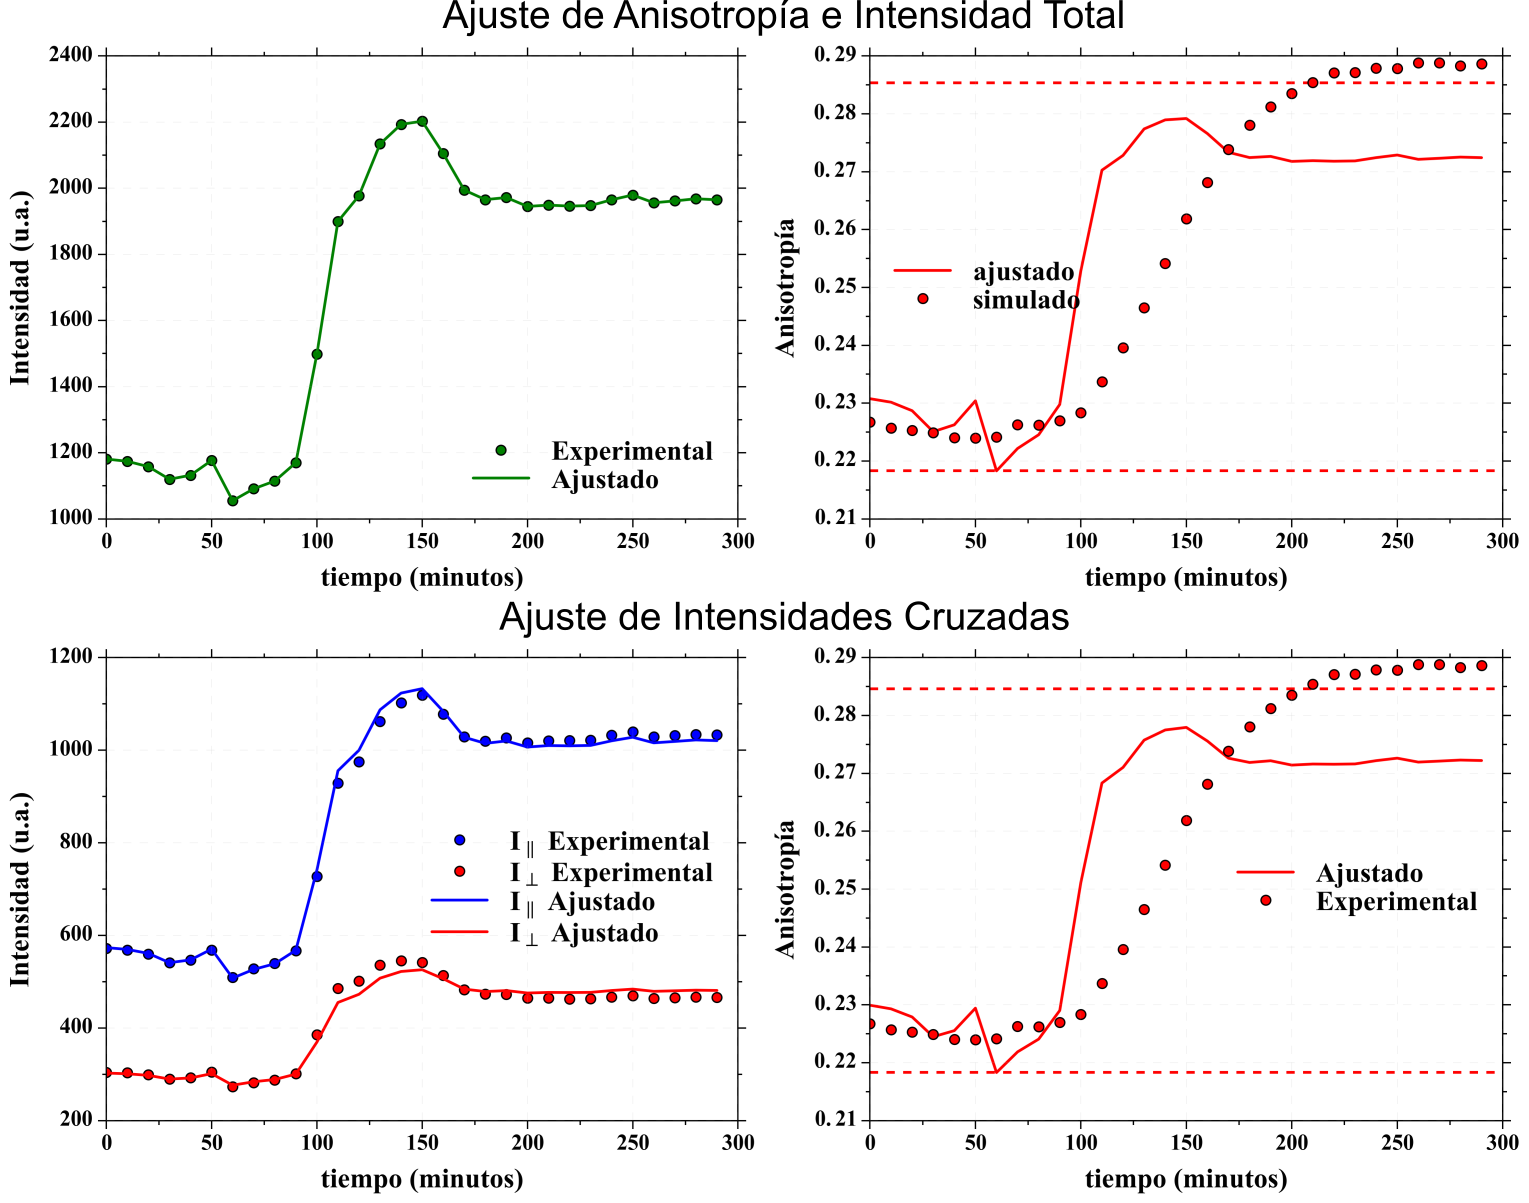
\includegraphics[width=0.9\textwidth]{./img/Cap4/Bad_Fits.png}
    \caption{Ajustes realizados sobre las curvas de anisotropía e intensidad total y sobre las intensidades cruzadas. Puede apreciarse que hay una elevada similitud entre las curvas ajustadas y las intensidades, pero cuando se analiza la anisotropía obtenida a partir del ajuste, esta no se condice con los datos experimentales.}
    \label{fig:Bad_Fits}
\end{figure}

Considerando que al generar las curvas simuladas para probar los distintos métodos de ajuste se tuvo en cuenta únicamente el ruido en las intensidades observadas, pero no se consideraron las variaciones que producen diferentes segmentaciones de la imagen de la célula, fue necesario repensar el método de ajuste para poder anular los efectos que una máscara distinta tenían sobre las curvas halladas. Con el objetivo de eliminar todo parámetro de escala, ya que no agrega información al ajuste y su variación se relaciona con diferentes segmentaciones de la imagen, se decidió trabajar con las intensidades cruzadas normalizadas por la intensidad total. Como se mostró en el capítulo \ref{cap:microscopia}, este método es el mejor para transformar los observables fotofísicos en una única curva que describe el estado del ensamble de fluoróforos.

En la figura \ref{fig:I_norm_Fit} se presenta un ajuste típico de estas curvas de intensidades cruzadas normalizadas. Puede apreciarse la elevada similitud entre ambas curvas al igual que si estudiamos la curva de anisotropía obtenida con su contraparte experimental. Se puede apreciar en la figura \ref{fig:m} la curva correspondiente de proporción de sensor en estado monomérico típica.

\begin{figure}
    \centering
    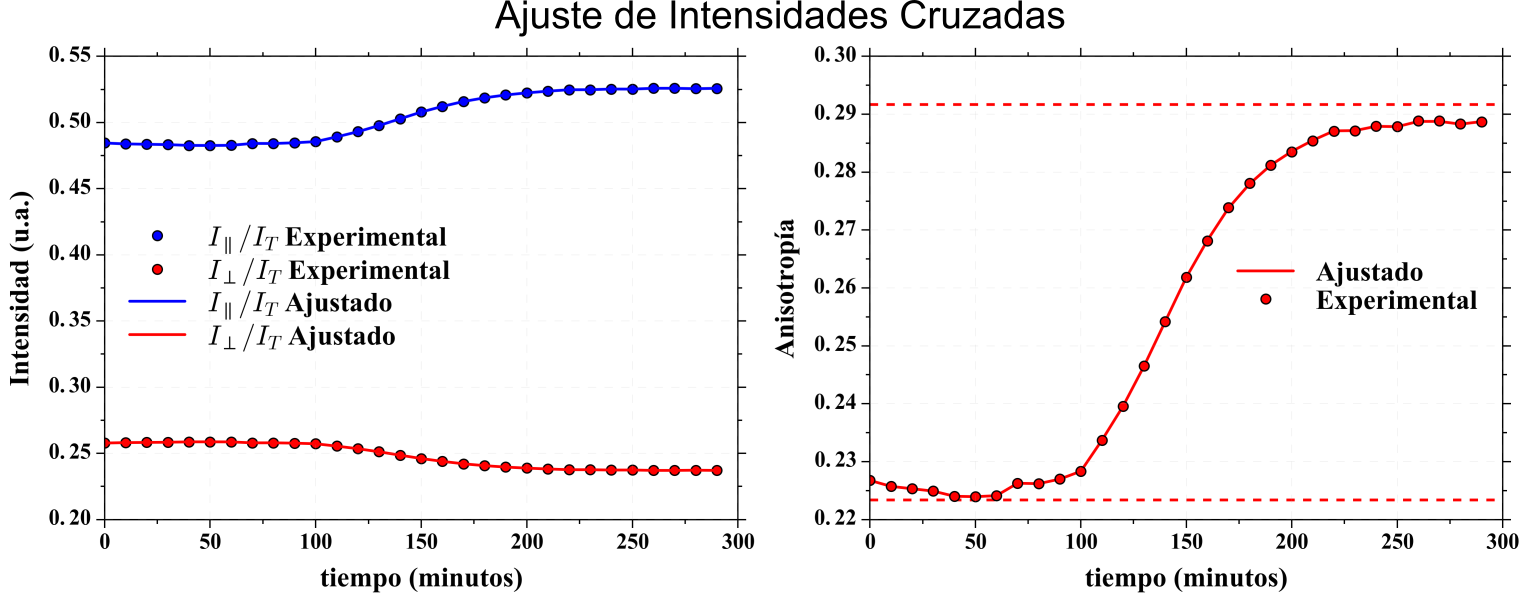
\includegraphics[width=0.9\textwidth]{./img/Cap4/Int_r_Fits.png}
    \caption{Ajustes realizados sobre las curvas intensidades cruzadas normalizadas. Puede apreciarse que hay la elevada similitud entre las curvas ajustadas y las intensidades, así como también entre la anisotropía obtenida a partir del ajuste y su contraparte experimental. Debe recalcarse que corresponde al ajuste de los mismos datos que la figura \ref{fig:Bad_Fits}}
    \label{fig:I_norm_Fit}
\end{figure}

\begin{figure}
    \centering
    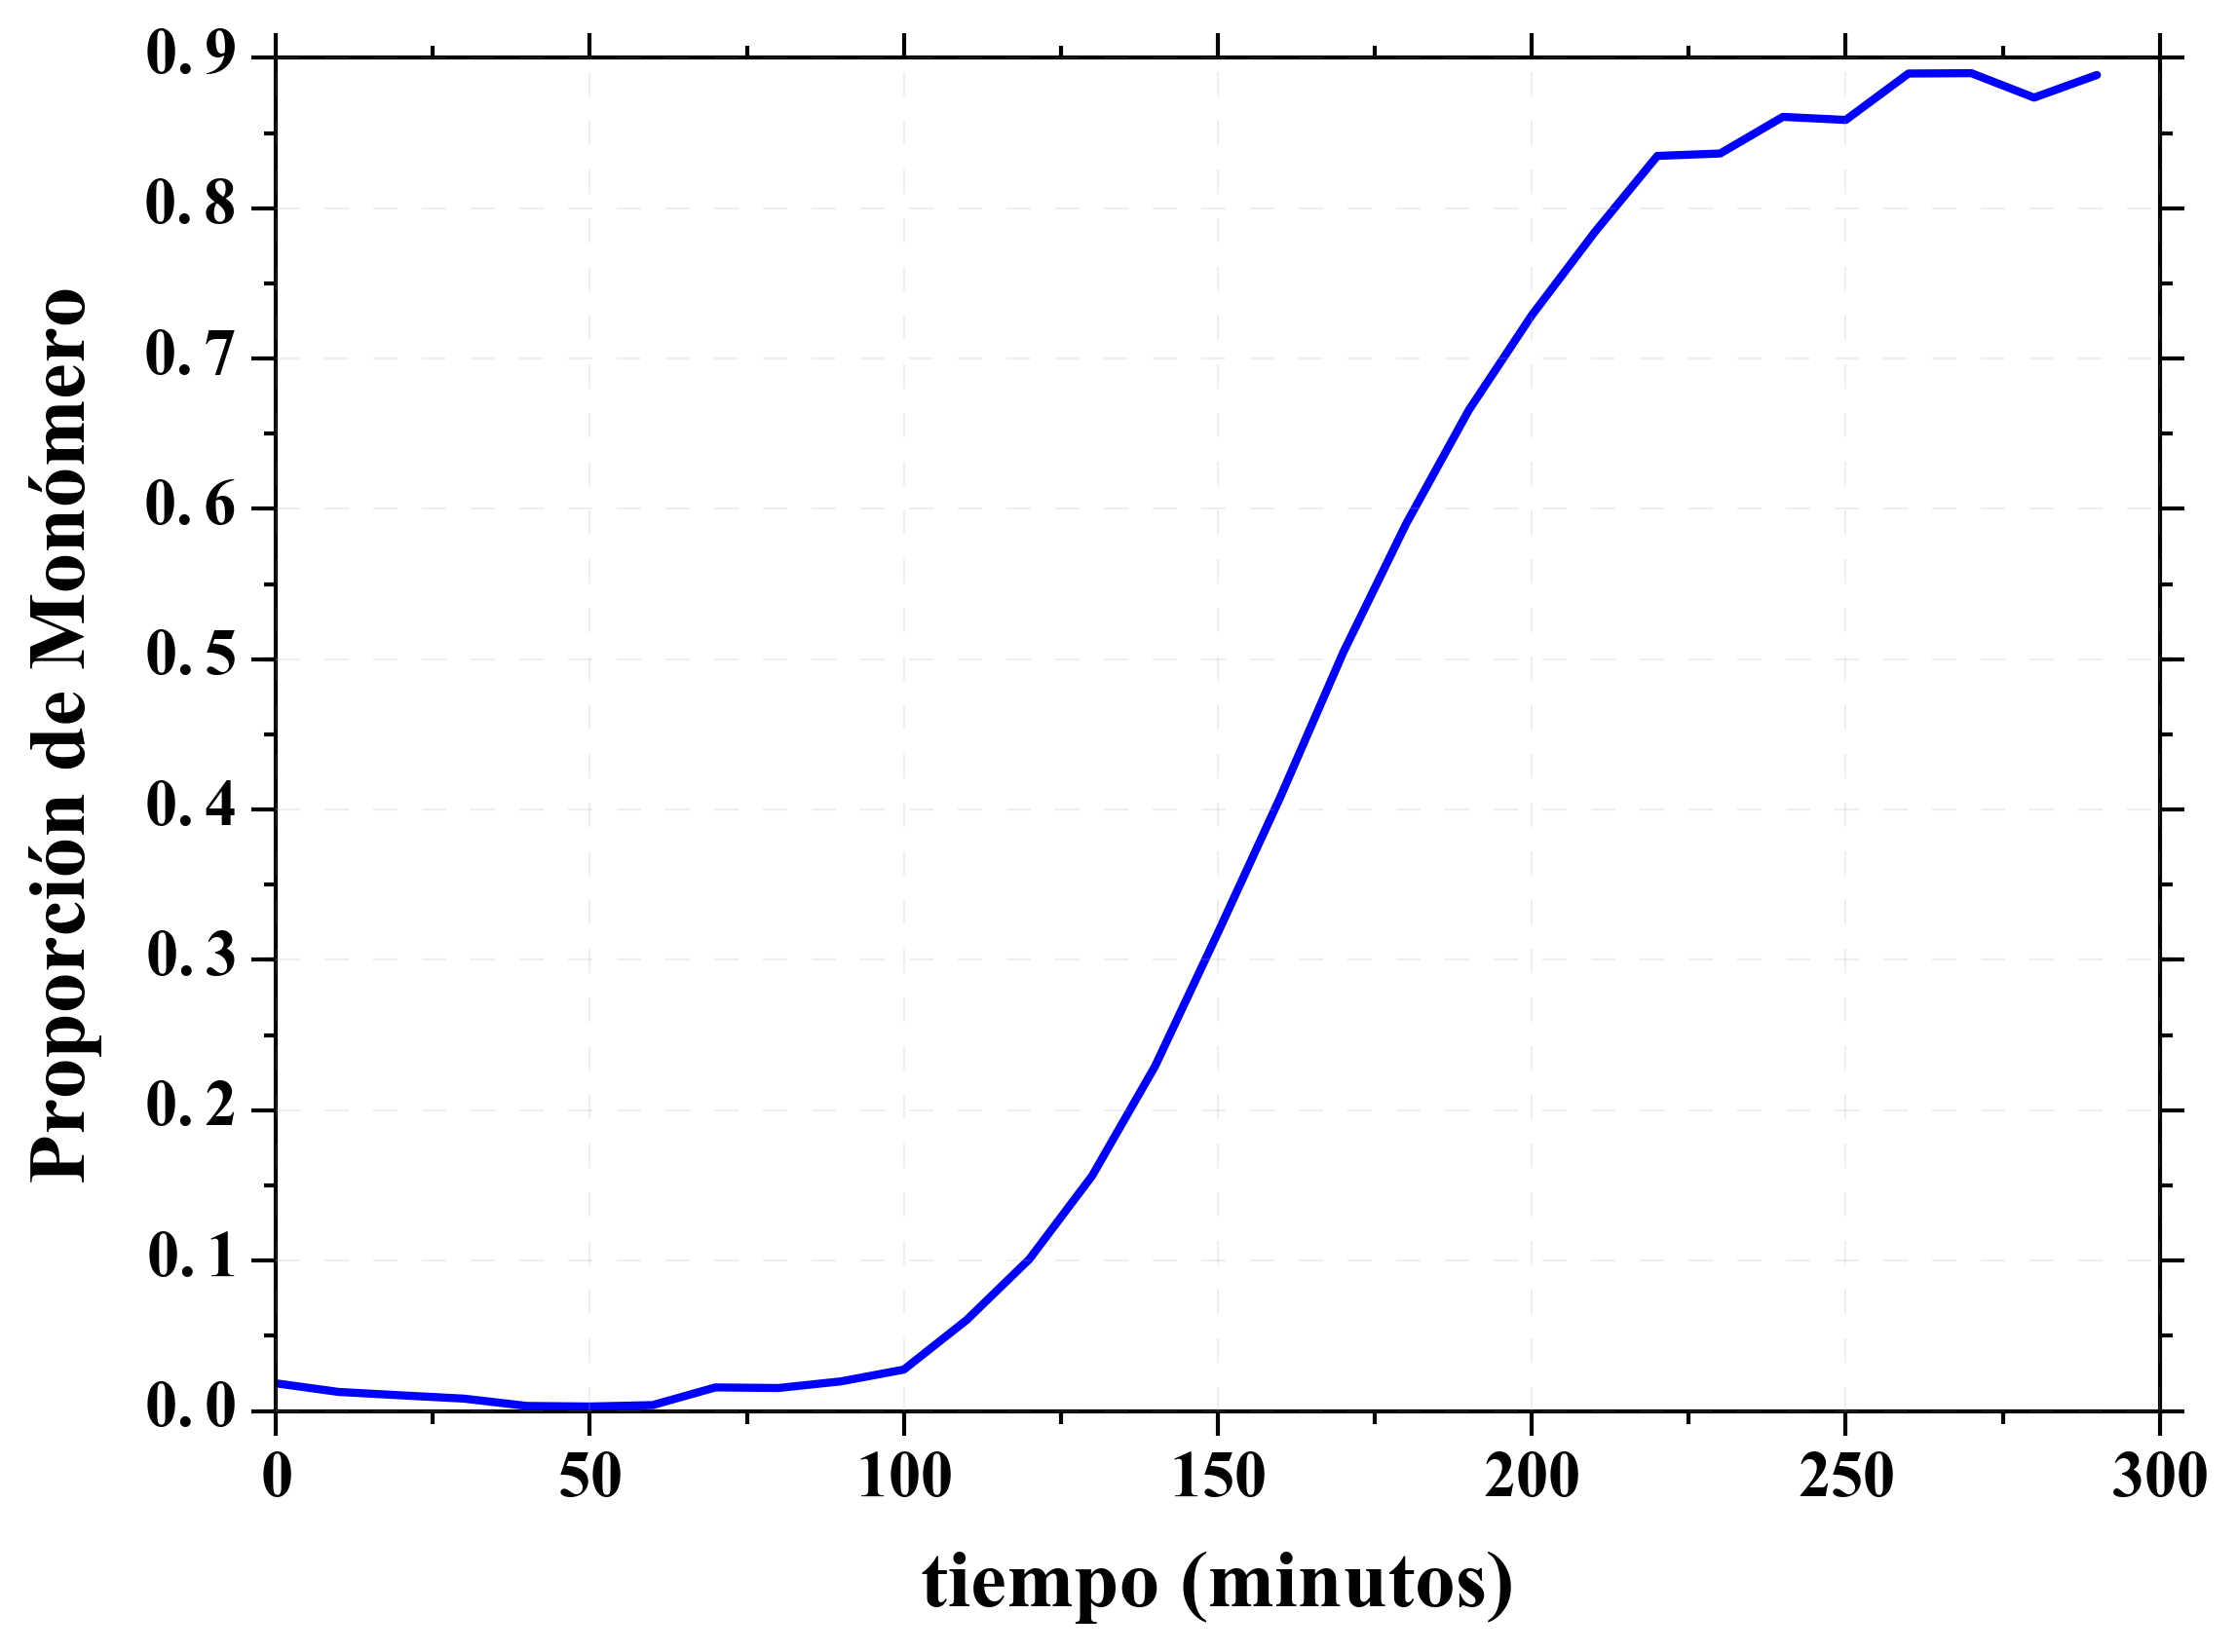
\includegraphics[width=0.6\textwidth]{./img/Cap4/Int_r_Fit_mYFP.png}
    \caption{Ajustes realizados sobre las curvas intensidades cruzadas normalizadas. Puede apreciarse que hay la elevada similitud entre las curvas ajustadas y las intensidades, así como también entre la anisotropía obtenida a partir del ajuste y su contraparte experimental.}
    \label{fig:m}
\end{figure}

%%%%%%%%%%%%%%%%%%
\section{Recuperación del Estado del Sistema Biológico}

Habiendo utilizado los hallazgos presentados en el capítulo \ref{cap:microscopia} para hallar las curvas de proporción de sensor en estado monomérico, se procedió a utilizar los métodos presentados en capítulo \ref{cap:modelo} para hallar el estado de la caspasa sensada. Luego, se procedió a calcular $\Delta m$ y $\Delta m/d$ como se mencionó previamente.

Con el objetivo de calcular $\Delta m$, se utilizó un filtro Savitzky-Golay para disminuir el ruido experimental y calcular la derivada temporal de $m$ utilizando más puntos que si utilizácemos un simple cálculo de cociente incremental. Aunque en muchos casos la curva obtenida no se condice con la teoría y aporta información del sistema, se pueden encontrar curvas como las presentadas en la figura \ref{fig:Deltams}. Esto genera problemas para estudiar diferencias en los tiempos de activación ya que muchas veces no podemos apreciar las curvas correspondientes a los tres sensores de una misma célula.

A continuación, se calcularon las curvas de $\Delta m/d$ para todas las curvas halladas. Desde el punto de vista numérico, este cálculo combina la problemática de calcular una derivada numérica con la necesidad de dividir por un factor que tiende a cero. Para evitar problemas al calcular divisiones por números chicos, se filtraron los valores de $d$ que eran considerados demasiado pequeños para el cálculo de $\Delta m/d$. De esta forma, se obtuvieron algunas curvas ideales, como la presentada en la figura \ref{fig:Deltams}, donde algunos puntos de la curva no pueden ser calculados, pero se puede apreciar gran parte del perfil de subida. El mayor inconveniente de estas curvas es que al no poseer información sobre los puntos más tardíos, cuando esta se normaliza, cambia la pendiente y no puede ser analizable.

\begin{figure}
    \centering
    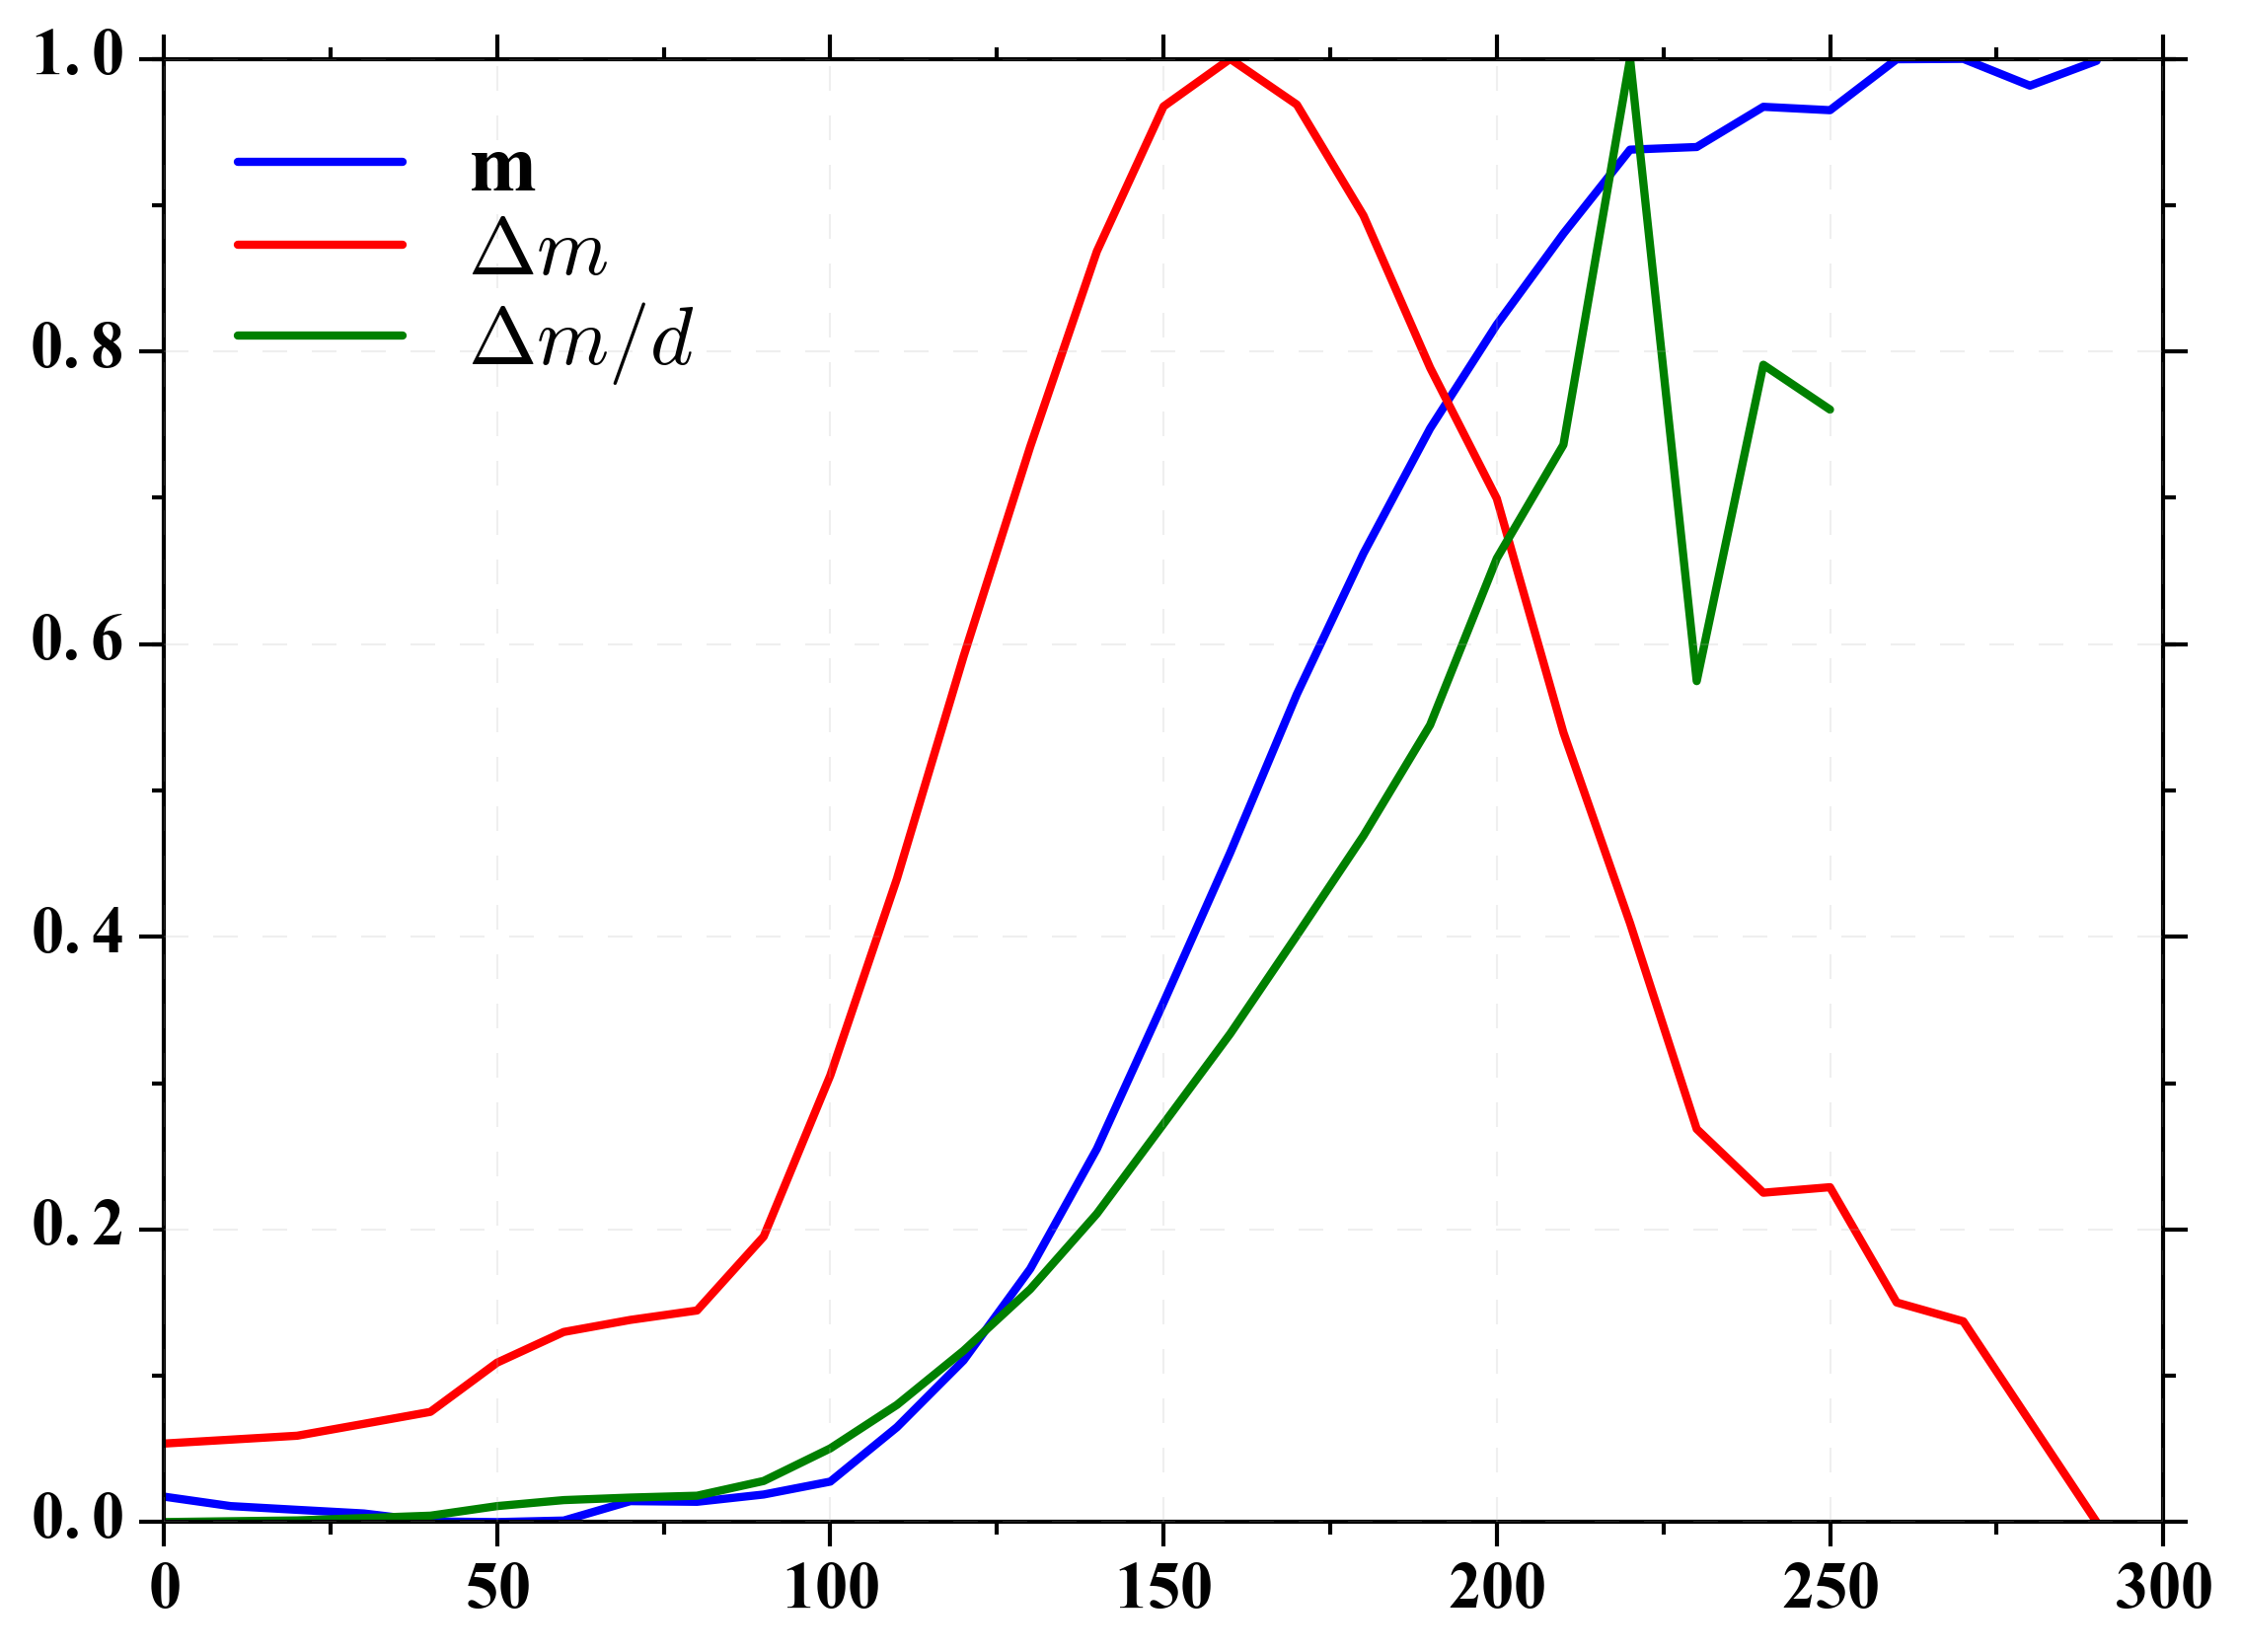
\includegraphics[width=0.6\textwidth]{./img/Cap4/Deltams.png}
    \caption{Gráfico de proporción de monómero en función del tiempo obtenido a partir de la transformación realizada. Se superponen los gráficos correspondientes a $\Delta m$ y $\Delta m/d$, que se corresponden a la caspasa en complejo con sensor y la proporción de caspasa activa en el momento.}
    \label{fig:m}
\end{figure}

Se planteó como corrección a futuro aumentar la resolución temporal para mejorar el cálculo de la derivada temporal. Debe considerarse que disminuir a la mitad el tiempo entre imágenes implica duplicar la cantidad de éstas, tornando más extenso el procesamiento de imágenes, u obligando a tomar imágenes de menos células. Por otro lado, los experimentos control que deben ser añadidos a la adquisición de imágenes permitirán determinar si el sensor comienza en estado dimérico en su totalidad, así como si culmina totalmente clivado. Esto puede ser utilizado para mejorar las aproximaciones sobre la curva de $d$ y así corregir aún más $\Delta m/d$.


%%%%%%%%%%%%%%%%%%%
\section{Ajuste Mediante Cinética Enzimática}

Con el objetivo de obtener una curva correspondiente a la proporción de caspasa activa, se diseño un método de ajuste de $m$ basado en cinética enzimática, presentado en la sección \ref{sec:CineticaEnzimatica}. Para ello, se truncó la cascada enzimática a nivel de la caspasa y solo se considero una fuente de caspasa tal que su proporción de caspasa activa, o enzima, poseía una forma funcional sigmoidea. Luego, los parámetros a ajustar correspondientes a la enzima son el tiempo en que la mitad de la enzima total aparece y la tasa de aparición de esta.

En este caso, la curva que se tiene disponible para ajustar es $m$, y los parámetros libres son los correspondientes a la aparición de enzima, así como todas las constantes de reacción. Debido a la gran cantidad de parámetros libres, resultaba fácil confeccionar ajustes que describan fielmente la forma de $m$, pero las curvas correspondientes a la caspasa que se obtenían eran extremadamente variables, y muchas veces carecían de sentido biológico.

Considerando que la cantidad de complejo sustrato:enzima es al menos cuatro ordenes de magnitud más chico que las cantidades de enzima, sustrato o producto (caspasa, dímeros o monómeros) y teniendo en cuenta que la velocidad de depleción de complejo es mucho mayor que la de sustrato, podemos aproximar la cinética enzimática de la siguiente forma

\begin{align}
    \frac{ds}{dt} =& - k_c se \label{eq:cin_sens}\\
    \frac{de}{dt} =& \nu(t)\\
    \frac{dp}{dt} =& 2 k_c se, \label{eq:cin_prod}\\
\end{align}

\noindent donde hay una única constante de reacción $k$ que combina todas las anteriores, y $\nu(t)$ corresponde a la fuente de enzima (caspasa) y es la derivada de la función sigmoidea, a saber,

\begin{equation}
    \nu(t) = A k \frac{e^{-k(t-t_0)}}{1 + e^{-k(t-t_0}},
\end{equation}

\noindent donde $A$ es la amplitud, tomada como 1 ya que corresponde a proporción de caspasa activa, $k$ es la tasa de aparición de caspasa, mientras que $t_0$ es el momento en que ya apareció la mitad de la caspasa activa.

Con el objetivo de validar este método de ajuste donde se varían los parámetros de la cinética enzimática hasta obtener la curva que mejor describe a $m$, se filtraron y analizaron datos correspondientes a un experimento control. Este consistió en diseñar los biosensores de forma tal que en una misma célula todos los biosensores sean clivados por la misma caspasa. De esta forma, se obtuvieron curvas de anisotropía para células que expresaban los tres sensores, pero su secuencia específica de clivaje es reconocida únicamente por la caspasa-3 u -8.

Si se tiene en cuenta que la caspasa tiene la misma constante de reacción para todos los sensores que tienen la secuencia específica reconocida por ella, se espera que los tres sensores se activen simultáneamente y tengan los mismos tiempos de activación. Podemos apreciar en la figura \ref{fig:OneCasp_Fit_m} las curvas de caspasa que se obtienen luego de ajustar las curvas de proporción de monómero. Al mismo tiempo, se presenta un gráfico del ajuste para tres pares de fluoróforos de la misma célula, mostrando la superposición entre estos.

\begin{figure}
    \centering
    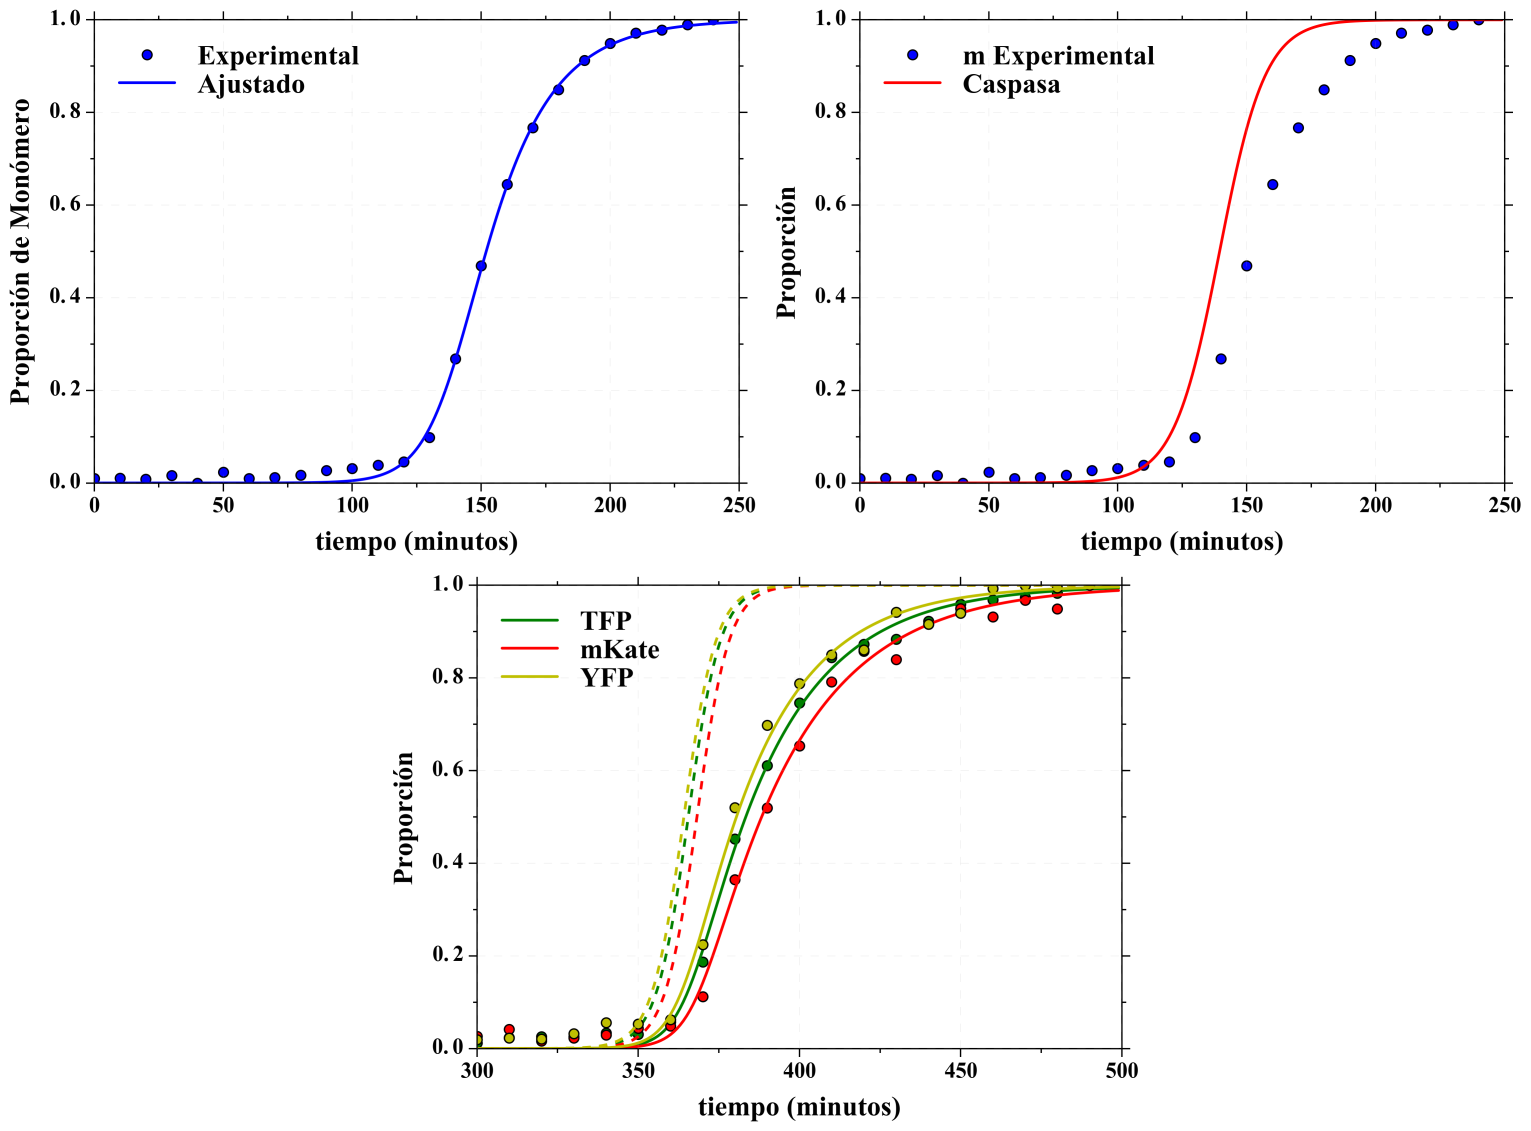
\includegraphics[width=0.9\textwidth]{./img/Cap4/OneCasp_Fit_m.png}
    \caption{Gráfico de los datos obtenidos de la proporción de sensor en estado monomérico. Se superponen el ajuste mediante cinética enzimática del cual se obtuvieron la proporción de monómero ajustada y la proporción de caspasa activa. En la sección inferior se presentan los ajustes realizados sobre tres caspasas de la misma célula, mostrando la validación del método con el caso control.}
    \label{fig:OneCasp_Fit_m}
\end{figure}

A continuación para validar este método, será necesario corroborar que los tiempos de activación, definidos como el tiempo que tarda la curva en llagar a cierto porcentaje de su valor máximo son los mismos para todas las caspasas. Luego, se consideraron los tiempos de activación al 10$\%$ y al 50$\%$ para cada par de fluoróforos y se graficaron uno contra otro. A partir de estos conjuntos de puntos, se calcularon las correspondientes regresiones lineales y se presentan sus gráficos en la figura \ref{fig:OneCasp_reg}. Los valores obtenidos para la regresión lineal correspondiente a usar el tiempo de activación de caspasa al 10$\%$ fueron para TFP contra YFP $-10.7 \pm 9.2$ de ordenada al origen y $1.02 \pm 0.03$ de pendiente; y para TFP contra mKate $-5.30 \pm 5.82$ de ordenada al origen y $1.01 \pm 0.02$ de pendiente. Por otro lado, utilizando la caspasa al 50$\%$ como tiempo de activación se aprecian para TFP contra YFP $-11.48 \pm 15.78$ de ordenada al origen y $1.03 \pm 0.05$ de pendiente, mientras que para TFP contra mKate se obtuvieron $2.45 \pm 9.95$ de ordenada al origen y $0.97 \pm 0.03$ de pendiente. En resumen, estos casos se superponen con la recta identidad que significa que este método es consistente al detectar la activación de la caspasa por igual para los tres sensores.

%p0 = -10.74 \pm 9.21
%p1 = 1.02 \pm 0.03


%p0 = -5.30 \pm 5.82
%p1 = 1.01 \pm 0.02


%p0 = -11.48 \pm 15.78
%p1 = 1.03 \pm 0.05


%p0 = 2.45 \pm 9.95
%p1 = 0.97 \pm 0.03

\begin{figure}
    \centering
    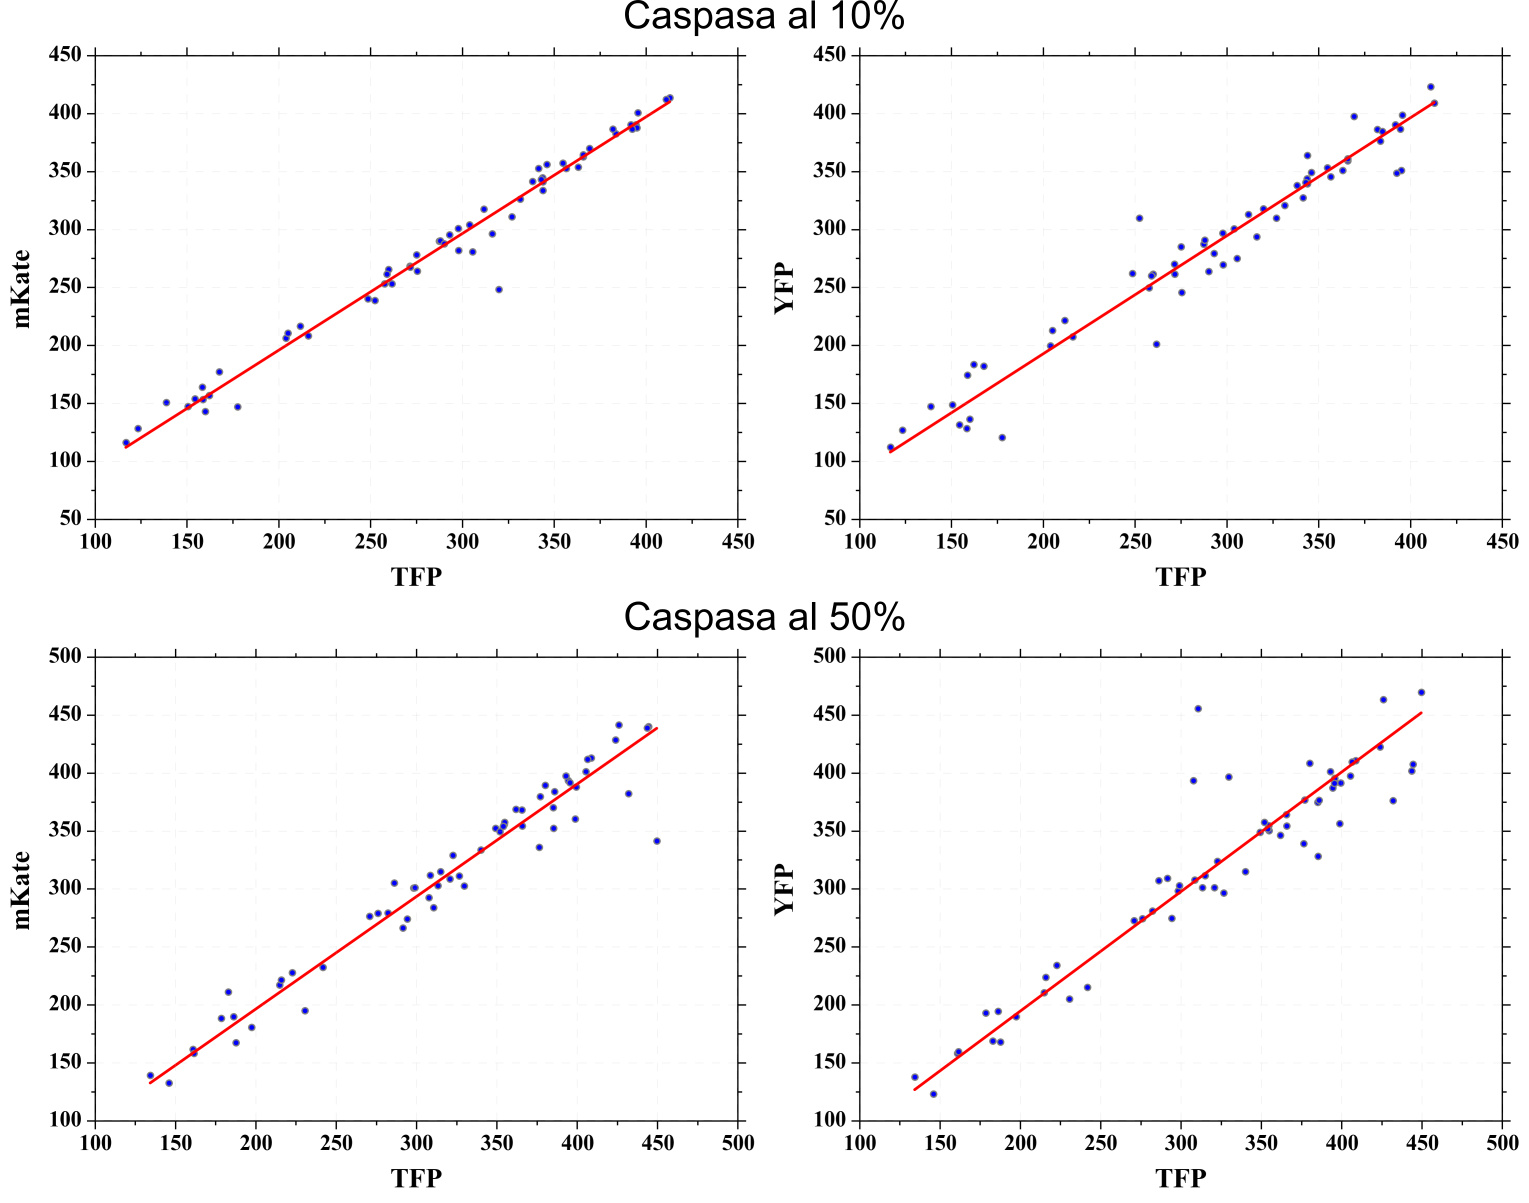
\includegraphics[width=0.9\textwidth]{./img/Cap4/CaspReg.png}
    \caption{Se graficaron los tiempos de activación obtenidos para 10$\%$ o 50$\%$ de activación de caspasa uno contra otro. La regresión lineal de estos datos permite constatar que efectivamente se trate del mismo parámetro ya que cada sensor medía la misma caspasa.}
    \label{fig:OneCasp_reg}
\end{figure}

%Por otro lado, es interesante comparar el método de tiempos de activación de caspasas con utilizar únicamente la anisotropía. Aunque ya mostramos que esto no es correcto ya que ignora varios fenómenos que dan lugar a variaciones en las curvas de anisotropía, . Entre estos, está el efecto que una relación entre brillos ($b$) distinto de 1 tiene sobre la pendiente de esta curva.

Por otro lado, podríamos retroceder y utilizar únicamente las curvas de anisotropía para encontrar en que momento asciende un 10$\%$ o 50$\%$ de su amplitud. Aunque se mostró en el capítulo \ref{cap:microscopia} que hacer esto implica ignorar efectos como, la variación de pendiente producida por una relación de brillos ($b$) distinta a 1, veamos si de todas formas es consistente y solo tiene un sesgo respecto del otro método. Para 10$\%$ de anisotropía se obtuvieron para TFP contra YFP $-21.26 \pm 8.95$ de ordenada al origen y $1.06 \pm 0.03$ de pendiente; para TFP contra mKate se obtuvo $-14.71 \pm 7.65$ de ordenada y $1.05 \pm 0.03$ de pendiente. Mientras que si utilizamos 50$\%$ de ascenso se obtienen para TFP contra YFP $-12.14 \pm 5.92$ de ordenada y $1.02 \pm 0.02$ de pendiente y para TFP contra mKate $-13.57 \pm 5.73$ de ordenada y $1.03 \pm 0.02$ de pendiente. Dado que en general hay una desviación respecto de la recta identidad, esto muestra que utilizar  los tiempos de activación obtenidos a partir de las caspasas es más robusto y consistente.

%p0 = -21.26 \pm 8.95
%p1 = 1.06 \pm 0.03


%p0 = -14.71 \pm 7.65
%p1 = 1.05 \pm 0.03


%p0 = -12.14 \pm 5.92
%p1 = 1.02 \pm 0.02


%p0 = -13.57 \pm 5.73
%p1 = 1.03 \pm 0.02

\begin{figure}
    \centering
    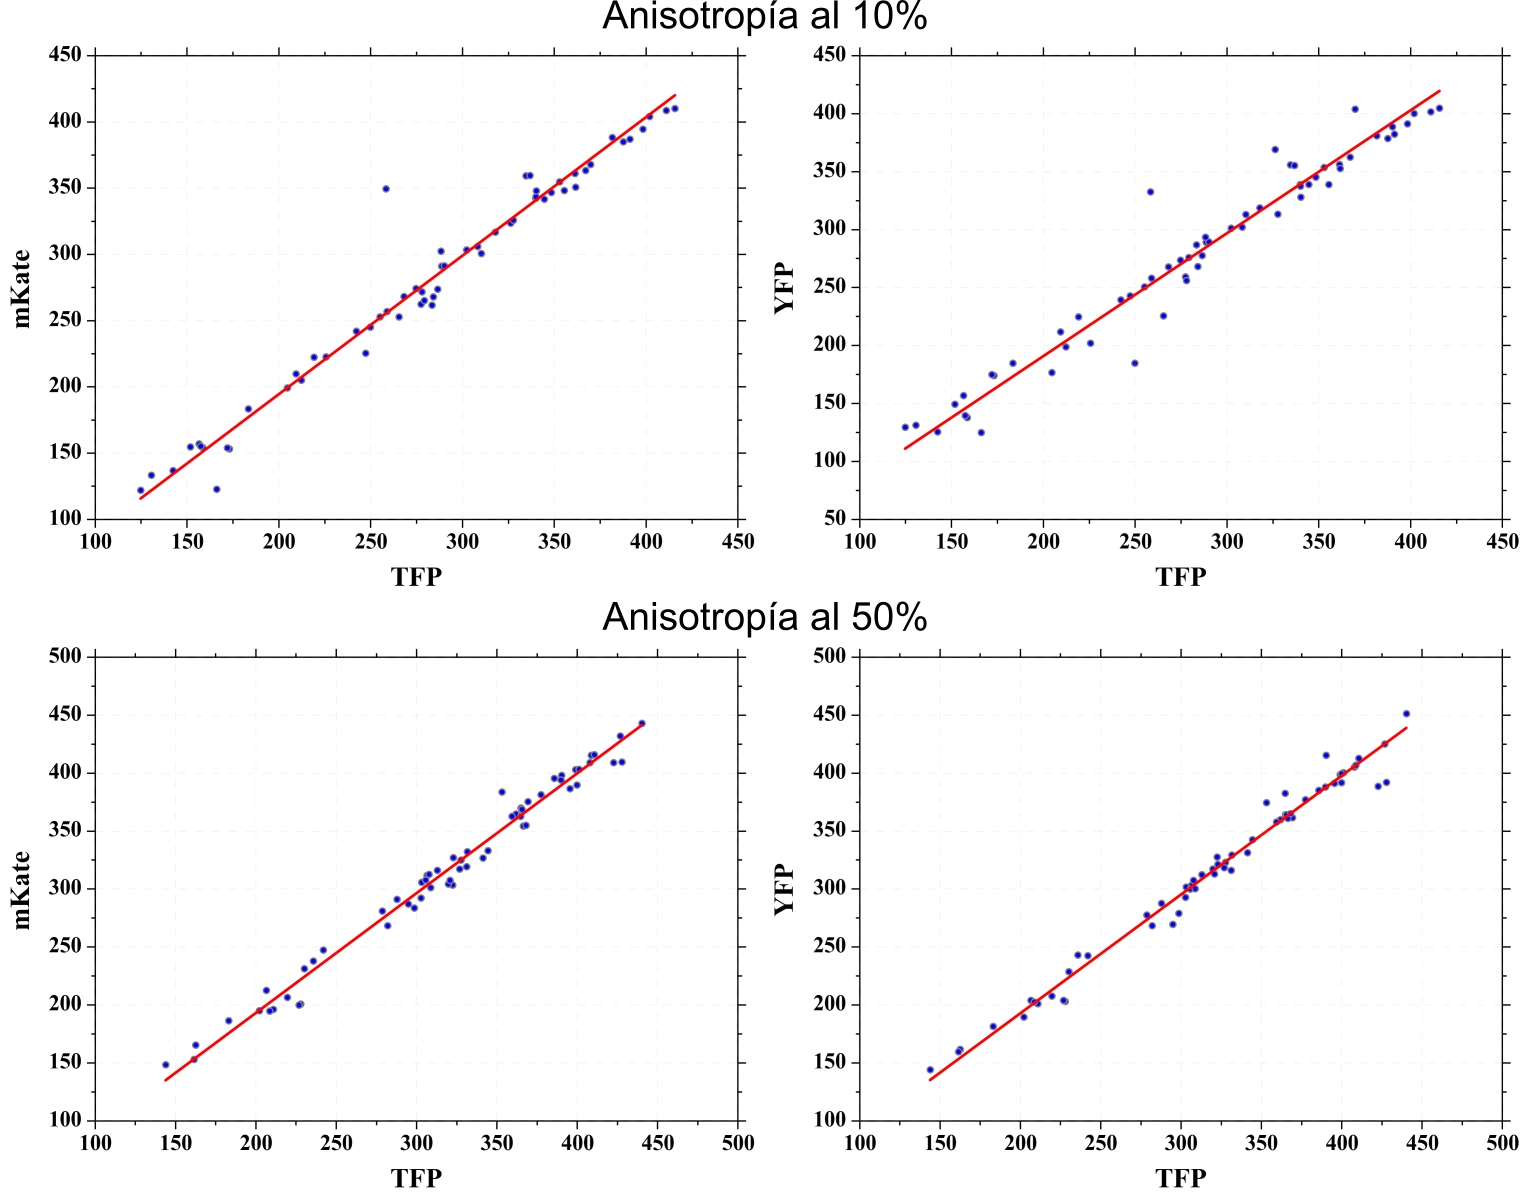
\includegraphics[width=0.9\textwidth]{./img/Cap4/AnisReg.png}
    \caption{Se graficaron los tiempos de activación obtenidos para 10$\%$ o 50$\%$ de activación de anisotropía uno contra otro. La regresión lineal de estos datos permite constatar que efectivamente se trate del mismo parámetro ya que cada sensor medía la misma caspasa.}
    \label{fig:OneCasp_reg_anis}
\end{figure}

%A partir de las regresiones lineales presentadas en las figuras \ref{fig:OneCasp_reg} y \ref{fig:OneCasp_areg}, podemos concluir que los ajustes mediante las simulaciones de cinética enzimática, no solo brindan información valiosa sobre el estado del sistema, sino que también son más robustas para comparar tiempos de iniciación.


%%%%%%%%%%%%%%%%%%%%%%
\section{Tiempo de Activación}

\subsection{Tiempos de Activación Observados}
Luego de validar el ajuste mediante las simulaciones de cinética enzimática, se procedió a aplicar el procedimiento a todas las curvas halladas experimentalmente. De este análisis fue posible obtener los tiempos de activación definidos previamente para las caspasas-3, -8 y -9 en una misma célula. Como se detalla en el trabajo de \textit{Sorger et al.}\cite{Sorger2008}, el tiempo en que se inicia la cascada apoptótica es muy variable intercelularmente, pero el orden y la diferencia entre los tiempos de activación de cada caspasa se mantiene relativamente constante entre las distintas células. Por esta razón, en lugar de analizar estadísticamente los tiempos de activación de las distintas caspasas, se estudiaron las diferencias entre los tiempos de activación.

\begin{figure}
    \centering
    \includegraphics[width=0.9\textwidth]{./img/Cap4/HistTimes.png}
    \caption{Se presentan histogramas de las diferencias entre los tiempos de activación de cada caspasa. }
    \label{fig:OneCasp_reg_anis}
\end{figure}

Al analizar los tiempos de activación al 10$\%$ se apreció que hay una diferencia temporal de $17.4\pm4.8$ desde la caspasa-8 a la -3, $21.8\pm5.0$ desde la -9 a la -8 y, por último, $40.6\pm5.6$ desde la caspasa-9 a la -3. Por otro lado, si consideramos el tiempo de activación como el momento en que el 50$\%$ de la caspasa se haya activa se obtuvieron diferencias de tiempo desde la caspasa-8 a la -3 de $18.8\pm4.5$, desde la caspasa-9 a la -8 de $42.2\pm6.0$ y de la caspasa-9 a -3 de $57.9\pm6.4$. De estos resultados puede deducirse que la caspasa-3 es la primera en iniciarse, seguida de cerca por la caspasa-8, y un tiempo después la caspasa-9. Se debe destacar que si prestamos especial atención a ambos estimadores, apreciamos que la caspasa-8 comienza temprano con la caspasa-3, pero luego se retrasa y alcanza su 50$\%$ de activación unos minutos antes que la caspasa-9.


\subsection{Tiempos de Activación Estimados}

A partir del modelo matemático adapatado en el capítulo \ref{cap:modelo}, podemos estimar la separación temporal entre las activaciones del 10$\%$ o 50$\%$ de caspasas. En primer lugar, cabe destacar que aunque parezca incoherente con el esquema de la red, la primer caspasa en llegar a una activación del 10$\%$ es la caspasa-3, seguida de cerca temporalmente por la caspasa-8. Un tiempo más prolongado, comparado con la separación entre las caspasas-3 y -8, separa a la activación del 10$\%$ de la caspasa-9. Experimentalmente podemos apreciar que el orden se conserva, aunque la separación entre las activaciones observadas experimentalmente son equiespaciadas.

Por otro lado, si analizamos las separaciones temporales entre las activaciones del 50$\%$ de caspasa, podemos apreciar que se invierten los ordenes de activación entre las caspasas-8 y -9, siendo la caspasa-3 la primera en activarse.En este caso, apreciamos en el experimento que la caspasa-8 sufre un retraso o la caspasa-9 se adelanta, como se explico previamente, pero este efecto no es suficiente para obtener una inversión en el orden de activación de las caspasas.


%%%%%%%%%%%%%%%%%%%%%%
\section{Orden de Activación Según Estímulo}

Hasta ahora, se consideró como estímulo un ligando que actúa a nivel de los receptores de muerte, como TNF-$\alpha$. El estímulo utilizado en los experimentos realizados fue la staurosporina. Aunque no hay certeza sobre la vía estimulada por la misma, los datos experimentales presentados y analizados sugieren que se trata de una estimulación de la vía extrínseca.

Con el objetivo de contrastar el orden de activación de las caspasas según que vía se ve estimulada, se generó una variante del modelo matemático que no contiene ligando para actuar a nivel del receptor. Por otro lado, en esta variante, parte de la proteína Bax comienza activa para inicializar la vía intrínseca. Bax esta involucrada en la respuesta celular a daño interno por especies reactivas del oxígeno.

\begin{figure}
    \centering
    \includegraphics[width=0.8\textwidth]{./img/Cap4/IntAct.png}
    \caption{Gráficos de proporción de caspasa activa y sensor sin clivar en función del tiempo para las tres caspasas de interés. En esta simulación se estimuló la vía intrínseca en lugar de la extrínseca y puede apreciarse una alteración en el orden en que se activan las caspasas.}
    \label{fig:IntAct}
\end{figure}

En esta variante de iniciación de vía intrínseca, se aprecia que la caspasa-9 alcanza primero el 10$\%$, así como también el 50$\%$ de activación primera. Un tiempo después la sigue la caspasa-3, mientras que la caspasa-8 es la última en llegar a los porcentajes de activación seleccionados. Estas diferencias en los ordenes de activación nos permiten determinar cual es la vía de entrada en apoptosis tomada por la célula.


%%%%%%%%%  Conclusión
\chapter{Conclusiones y Discusiones}

A lo largo del presente trabajo se mostraron una serie de variantes a los métodos para analizar señales fotofísicas provenientes de experimentos basados en dinámica de sensores de homoFRET. Entre estos métodos, se mostró la mejor forma de transformar los observables experimentales (intensidades cruzadas) para recuperar el estado del ensamble del fluoróforo instante a instante. A continuación, se presentó un modelo matemático, con su correspondiente adaptación, que se utilizó para estudiar el comportamiento de los elementos del sistema biológico. A partir de este, fue posible diseñar un análisis que permite obtener el estado de la variable biológica de interés haciendo uso únicamente de la información provista por el sensor.

Luego de unir el desarrollo realizado en métodos de análisis de datos experimentales con el correspondiente al modelado del sistema biológico se procedió a analizar datos provenientes de un experimento. La aplicación de estos métodos a un experimento real sirvió como prueba de concepto de los métodos presentados.

%\section{Conclusión}

En primer lugar, se detallaron las razones por las que un análisis robusto de la señal de anisotropía debe comprender una transformación de los datos experimentales en información sobre el ensamble de fluoróforos. Debido a que el brillo de un monómero en estado asociado (dímero) o disociado (monómero) es distinto, es necesario utilizar ambos observables experimentales para estudiar el estado del ensamble de fluoróforos. Esta diferencia en brillos no se debe únicamente a diferencias en la detección de los distintos fluoróforos, ya sea por diferencias en emisión, rendimiento cuántico o distinta respuesta del canal de detección para longitudes de onda distintas, sino que también pueden darse diferencias en la maduración de los fluoróforos apareados. Al ocurrir transferencia de energía entre fluoróforos, la intensidad de fluorescencia detectada también variará, incluso cuando la cantidad de fluoróforoso de cada especie sea la misma.

%cuando estos se hallan asociados y hay transferencia de energía entre ellos, el canal de detección detecta a ambos con el mismo brillo ya que sus diferencias en espectro, combinados con los filtros del sistema óptico, generan monómeros con brillos distintos.

%Es usual hallar en la bibliografía que se ajustan las curvas de anisotropía utilizando funciones sigmoideas y se toman como parámetros relevantes la velocidad de transición, así como el tiempo en que se alcanza la mitad del rango de anisotropía. Como se mostró en el capítulo \ref{cap:microscopia}, este método no debe utilizarse cuando el fluoróforo presenta brillos distintos según este asociado o disociado.

%siempre resulta el más conveniente debido a que se trunca el análisis a nivel de la señal fotofísica, sin indagar en el estado del ensamble de fluoróforos, ni en el estado del sistema biológico en estudio.



%Una vez desarrollado el método para transformar las intensidades cruzadas en información del estado del ensamble de fluoróforos y el 

En el capítulo \ref{cap:microscopia}, se mostraron métodos que ajustaban tanto los observables directos, intensidad paralela y perpendicular, como un método que utilizaba una combinación de estos observables que eran la anisotropía y la fluorescencia total. En ambos métodos, era necesario ajustar un parámetro de escala para la intensidad de fluorescencia. Posteriormente, se mostró que ajustarlo trae aparejado el inconveniente que diferencias en la segmentación de las imágenes causan aumentos repentinos de las intensidades que complican el ajuste de los datos experimentales. Con el objetivo de corregir este problema, se planteó como solución ajustar las intensidades cruzadas normalizadas por la intensidad total del sistema.

Ajustar las curvas de intensidades cruzadas normalizadas nos provee ventajas desde varias perspectivas distintas. Teóricamente, elimina el parámetro de escala de todos los ajustes. Desde el punto de vista experimental, este método elimina efectos generados por problemas en la segmentación de imágenes para analizar. Por último, provee la transformación más fiel de los datos experimentales a la curva que determina el estado del ensamble de fluoróforos.

%1. Teoricamente nos sacamos de encima parametro de escala
%2. EN simulaciones es el mas fiel para ajustar la anisotropía, pero traduce todo el ruido en m
%3. En datos reales lo mostramos con el experimento 3sensores:1caspasa, sale de la regresion lineal, ademas de la explicacion de como nos desentendemos de los problemas  de segmentacion de imagenes

Entre los problemas que presentó el ajuste de las intensidades cruzadas observadas se encuentra el desconocimiento de muchos de los parámetros involucrados. Por un lado, el parámetro $b$ que relaciona el brillo de un monómero en estado asociado con el brillo del monómero disociado puede calcularse experimentalmente mediante experimentos de \ening{N\&B}. En segundo lugar, se recomienda generar células que expresen biosensores no clivables, así como otro grupo de células que expresen sensores clivados en su totalidad para obtener mediciones de las anisotropías máxima y mínima en que puede variar la anisotropía de un par de fluoróforos. Como se explicó previamente, no alcanza con determinar estos valores teóricamente ya que se observaron errores sistemáticos distintos en las anisotropías máximas y mínimas observadas experimentalmente.

En el capítulo \ref{cap:modelo}, se adaptó el modelo matemático desarrollado por \textit{Sorger et al.}\cite{Sorger2008} para que describa adecuadamente el comportamiento de los sensores transfectados a la célula. Se concluyó el capítulo mostrando diversas técnicas numéricas que permitían identificar el estado de variables de interés biológico. Estas variables son la cantidad de complejo caspasa:sensor que esta íntimamente relacionada con la actividad de la caspasa en cada instante, y la proporción de caspasa activa. Por otro lado, debemos recalcar que estos métodos numéricos no pudieron ser aplicados a todas las curvas. Para contrarrestar estos inconvenientes se recomienda mejorar la resolución temporal, con el objetivo de facilitar el cálculo de la derivada temporal de la curva de proporción de sensor en estado monomérico; y por otro lado, utilizar los experimentos control mencionados previamente para confeccionar un mejor filtrado de los puntos en que la curva de proporción de sensor en estado dimérico es muy baja.

Con el objetivo de obtener información sobre el estado de la caspasa a partir de la curva de proporción de monómero, se plantearon ajustes de esta curva a partir de simulaciones de cinética enzimática. A continuación, se validó dicho método mediante su aplicación a un experimento control. Este método fue útil para obtener las curvas de proporción de caspasa activa de las curvas experimentales en estudio para luego estimar los tiempos de activación de cada caspasa. Estos resultados fueron contrastados posteriormente con el orden de activación predicho por el modelo teórico donde se apreció una elevada concordancia para el tiempo de activación de caspasa al 10$\%$. Las diferencias en separación temporal o en orden de activación al 50$\%$ pueden corregirse si se varían las condiciones iniciales del sistema.

En conclusión, se presentó en este trabajo un análisis exhaustivo de los datos experimentales que permite transformar el observable fotofísico, que son las intensidades cruzadas, en la proporción de caspasa activa, que representa la variable de interés biológico. Por otro lado, el modelo matemático adaptado no solo sirve para contrastar los datos experimentales observados, sino que predice cambios en el orden de activación de las caspasas ante distintos estímulos. Esto último, es el puntapié inicial para evaluar la respuesta del mismo sistema celular ante distintos estímulos y estudiar las diferencias en el orden de activación de las caspasas.


%%%%%%%%%  Agradecimientos
\setcounter{page}{1}
\pagenumbering{roman}
\thispagestyle{empty}
\chapter*{Agradecimientos}

En primer lugar, agradezco a Dios por haberme dado el espíritu y profundo deseo para estudiar la compleja maquinaria que es la vida, así como le agradezco el haber creado, con su clara impronta, esa maquinaria sin la cual siquiera hubiera podido comenzar a estudiar.

Quiero agradecer a toda mi familia por haberme enseñado y guiado desde temprano en mi vida, especialmente por apoyarme y darme más de lo que necesitaba para cumplir mis metas. Sin ella tendría una identidad completamente distinta y no sería quien soy. 

Al mismo tiempo, quiero agradecer especialmente a Marcela, mi futura esposa, en quien encontré la persona ideal a la que serle fiel. Su inconmensurable apoyo, infinita bondad e interminable paciencia me sirvieron de riel para encaminarme en la vida profesional, y espero que en un futuro se vean reflejados en nuestra vida familiar.

Asimismo, agradezco a todos mis amigos porque cada uno de ellos intercambió conmigo palabras y experiencias que de a poco me llevaron por los caminos que decidí andar. Como dijo la madre Teresa de Calcuta: \textit{somos una gota de agua en el océano, pero sin esa gota, el océano no sería el mismo}, y creo yo que lo mismo se aplica al océano de experiencias que uno tiene instante a instante, y nos van formando en nuestra personalidad.

Me alegra poder agradecer a Hernán, mi director, por su excelente didáctica y todas las enseñanzas que me dejó en estos años. Quiero agradecerle de antemano por todas las que vendrán en los próximos años. En particular, le agradezco a él y Klaus quienes me proveyeron de los datos experimentales que me mantuvieron fascinado durante todo este tiempo.

Finalmente, pero no menos importante, quiero agradecer a todos los miembros del laboratorio de electrónica cuántica. Sin ellos este verano inolvidable lo hubiese sido por razones opuestas. Sus oídos atentos estuvieron prácticamente todos los días para ofrecerme una ayuda cuando la necesitaba.

%Por último, les pido disculpas que no realicé un listado de uno por uno de todas las personas que agradezco. Todos saben lo importantes que fueron para mí, y por eso no creo necesario detallarlos en una extensa lista.

%%%%%%%%%%%%%%   Referencias   %%%%%%%%%%%%%%%%%%%%%%%%%%
\cleardoublepage
\bibliography{./Referencias.bib}
\bibliographystyle{ieeetr}

%\begin{figure}[H]
%    \centering
%    \includegraphics[width=0.49\textwidth]{resistencia.jpg}
%    \caption{\footnotesize{Valores de resistencia de la muestra en %función de la temperatura.}}  
%    \label{figResistencia}
%\end{figure}


%\begin{figure}[H]
%    \begin{subfigure}{0.49\textwidth}
%            \includegraphics[width=0.99\textwidth]{zoom2.jpg}
%            \caption{\footnotesize{Valores obtenidos de resistencia en %función de temperatura en un rango de $82.2$ °K a $82.8$ °K.}}
%            \label{figZoom2}
%    \end{subfigure}
%    
%    \begin{subfigure}{0.49\textwidth}
%       \includegraphics[width=0.99\textwidth]{fase2.jpg}
%        \caption{\footnotesize{Valores de fase obtenidos en función de %temperatura en un rango de $82.2$ °K a $82.8$ °K.}}
%        \label{figFase2}
%    \end{subfigure}
%
%    \caption{\footnotesize{Detalle de resistencia y fase medidas para la región de interes de $82.2$ °K a $82.8$ °K.}}
%    \label{figZona2}
%\end{figure}


%\begin{thebibliography}{10}


%\end{thebibliography}


\end{document}